% Retoca las líneas marcadas con TODO según las necesidades

\documentclass[oneside,a4paper,12pt]{book} % TODO: cambia "oneside" por "twoside" a la hora de imprimirlo

\usepackage[spanish]{babel}
\usepackage[utf8]{inputenc}
\usepackage{geometry}
\usepackage{makeidx}
\usepackage{url}
\usepackage{graphicx}
\usepackage{color}
\usepackage{caption}
\usepackage{acronym}
\usepackage{hyphenat}
\usepackage{a4wide}
\usepackage[normalsize]{subfigure}
\usepackage{float}
\usepackage{titlesec}
\usepackage[Lenny]{fncychap}
\usepackage{listings} % para poder hacer uso de "listings" propios (p.ej. códigos)
\usepackage{eurosym} % para poder usar el símbolo del euro con \euro {xx}
\usepackage{hyperref} % TODO: añade la opción hidelinks para imprimirlo (los enlaces no aparecerán resaltados)
\usepackage{array}
\usepackage{multirow}

% Para que no parta las palabras
\pretolerance=10000

\newcommand{\bigrule}{\titlerule[0.5mm]} \titleformat{\chapter}[display] % cambiamos el formato de los capítulos
{\bfseries\Huge} % por defecto se usaron caracteres de tamaño huge en negrita
{% contenido de la etiqueta 
\titlerule % línea horizontal 
\filright % texto alineado a la derecha 
\Large\chaptertitlename\ % capítulo e índice en tamaño large
\Large % en lugar de 
\Huge \Large\thechapter} 
{0mm} % espacio mínimo entre etiqueta y cuerpo
{\filright} % texto del cuerpo alineado a la derecha
[\vspace{0.5mm} \bigrule] % después del cuerpo, dejar espacio vertical y trazar línea horizontal gruesa
\geometry{a4paper, left=3.5cm, right=2cm, top=3cm, bottom=2cm, headsep=1.5cm}

% Estilos para ilustrar códigos:
\definecolor{code_green}{rgb}{0,0.6,0}
\definecolor{code_gray}{rgb}{0.5,0.5,0.5}
\definecolor{code_mauve}{rgb}{0.58,0,0.82}

\lstset{frame=tb,
  language=C,
  aboveskip=3mm,
  belowskip=3mm,
  showstringspaces=false,
  columns=flexible,
  basicstyle={\small\ttfamily},
  numbers=none,
  numberstyle=\tiny\color{code_gray},
  keywordstyle=\color{blue},
  commentstyle=\color{code_green},
  stringstyle=\color{code_mauve},
  breaklines=true,
  breakatwhitespace=true,
  tabsize=3
}

\lstset{frame=tb,
  language=C++,
  aboveskip=3mm,
  belowskip=3mm,
  showstringspaces=false,
  columns=flexible,
  basicstyle={\small\ttfamily},
  numbers=none,
  numberstyle=\tiny\color{code_gray},
  keywordstyle=\color{blue},
  commentstyle=\color{code_green},
  stringstyle=\color{code_mauve},
  breaklines=true,
  breakatwhitespace=true,
  tabsize=3
}

\lstset{frame=tb,
  language=Python,
  aboveskip=3mm,
  belowskip=3mm,
  showstringspaces=false,
  columns=flexible,
  basicstyle={\small\ttfamily},
  numbers=none,
  numberstyle=\tiny\color{code_gray},
  keywordstyle=\color{blue},
  commentstyle=\color{code_green},
  stringstyle=\color{code_mauve},
  breaklines=true,
  breakatwhitespace=true,
  tabsize=3
}

% Definición de mis propios tipos: Códigos, Ecuaciones y Tablas
\DeclareCaptionType{code}[Código][Listado de códigos]
\DeclareCaptionType{myequation}[Ecuación][Listado de ecuaciones]

% TODO: especifica las reglas de separación que consideres. Algunos ejemplos:
\hyphenation{fuer-tes}
\hyphenation{mul-ti-ca-pa}
\hyphenation{res-pues-ta}
\hyphenation{di-fe-ren-tes}
\hyphenation{de-sa-rro-lla-dos}
\hyphenation{re-pre-sen-tan-do}

 % archivo de configuración de estilo

\makeindex

\begin{document}
\baselineskip 1.35\baselineskip

\frontmatter

\thispagestyle{empty}
\vspace{2cm}

\begin{figure}[htb]
  \centerline{\resizebox{.60\textwidth}{!}{
\includegraphics{figs/logo_urjc}}}
\end{figure}

\begin{center}
  {\Large {\bf GRADO EN INGENIERÍA DE ROBÓTICA SOFTWARE}}
  \vspace{5mm}
 
  {\large {Escuela Técnica Superior de Ingeniería de Telecomunicación}}
  \vspace{5mm}

  {\large {Curso académico 2021-2022}}

  \vspace{1cm}

  {\large {\bf Trabajo fin de grado}}

  \vspace{2cm}

  {\Large {Sistema de detección de emociones faciales para\\
               un sistema robótico de bajo coste basado en ROS\\[1cm] }}

  \vspace{5cm}
  {\bf Autor}: Javier Martínez Madruga \\
  {\bf Tutor}: Julio Vega Pérez
\end{center}

\clearpage
\thispagestyle{empty}


% Este diseño se corresponde con la licencia CC-BY-NC-SA.
% Por supuesto, puedes poner la licencia que mejor se adapte al propósito de tu trabajo.
% Recuerda que, si no se especifica ninguna licencia, esta -como cualquier creación artística- pasaría a estar licenciada con todos los derechos reservados (copyright).

\vspace{5cm}

\begin{flushright}

\begin{figure}

\includegraphics[width=0.10\textwidth,right]{figs/by-nc-sa.png}
\end{figure}

\vspace{0.2cm}

{\tiny 
(CC) \textbf{Javier Martínez}\\ % TODO: pon aquí tu nombre cuando hagas el documento
\vspace{0.5cm}
\emph{
Este trabajo se entrega bajo licencia \href{https://creativecommons.org/licenses/by-nc-sa/3.0/es/}{CC BY-NC-SA}. \\
Usted es libre de \textit{(a) compartir}: copiar y redistribuir el material en \\
cualquier medio o formato; y \textit{(b) adaptar}: remezclar, transformar \\
y crear a partir del material. El licenciador no puede revocar estas \\
libertades mientras cumpla con los términos de la licencia. \\}
}

\end{flushright}



\cleardoublepage

\chapter*{Agradecimientos}

Unas bonitas palabras...\\

Quizás un segundo párrafo esté bien. No te olvides de nadie.\\

Un tercero tampoco viene mal para contar alguna anécdota...\\

¿Alguien más? Aunque sean \textit{actores} secundarios.\\

Un quinto párrafo como colofón.\\
\ % Algo de separación...

\

\

\

\

\begin{flushright}
		\vspace{4.0 cm}
		\emph{A alguien especial;\\
      si no, tampoco pasa nada}\\
		\par
		\vspace{1.0 cm}
		Madrid, xx de xxxxxx de 20xx\\ %\today
		\emph{Tu nombre}
\end{flushright}

\thispagestyle{empty}



\cleardoublepage

\chapter*{Resumen\markboth{Resumen}{Resumen}}

Escribe aquí el resumen del trabajo. Un primer párrafo para dar contexto sobre la temática que rodea al trabajo.\\

Un segundo párrafo concretando el contexto del problema abordado.\\

En el tercer párrafo, comenta cómo has resuelto la problemática descrita en el anterior párrafo.\\

Por último, en este cuarto párrafo, describe cómo han ido los experimentos.


\cleardoublepage

\chapter*{Abstract\markboth{Abstract}{Abstract}}

Service robotics ---a broad branch of research within robotics--- is characterized by offering useful services to humans. Within this branch we find Human Robot Interaction or HRI, a field of study that arises from the need for robots to be able to collaborate and live with us, humans. For this purpose, Artificial Vision plays a fundamental role, which, together with Machine Learning, provides the robot with qualities such as facial and emotion recognition, giving it capabilities that allow it to interact appropriately according to the context.\\

Machine Vision tasks that make use of Machine Learning, usually demand a high computational load, and not all robot developers have enough money or even space within their automatons to get a large computational station. That is why in this work we have developed an emotion detection tool capable of running in a low-cost system, that is, in an embedded system characterized by its small size and low price.\\

Emotion detection has been carried out by training classification algorithms (KNN, SVM and MLP) with angular data extracted from facial expressions produced by human emotions (anger, happy, sadness and surprise). The angular data have been obtained from the construction of an \textit{emotional mesh}, from facial points, based on the Facial Coding System (FACS). The hardware used has been the Raspberry Pi 4 Model B board, and the final tool has been integrated in ROS Noetic to facilitate its use in robotic systems.\\

Several studies have been carried out in order to find the best optimization for the tool, as well as to perform final tests to verify its operation and performance in frames per second.

\cleardoublepage

\chapter*{Acrónimos\markboth{Acrónimos}{Acrónimos}}

% Añade a continuación los acrónimos que uses en el documento. Algunos ejemplos:
\begin{acronym}
	\acro{RUR}{\emph{Rossum's Universal Robots}}
	\acro{IFR}{\emph{Federación Internacional de Robótica}}
	\acro{AGV}{\emph{Vehículo Guiado Automático}}
	\acro{AMR}{\emph{Robot Móvil Autónomo}}
	\acro{HRI}{\emph{Interacción humano-robot}}
	\acro{SVM}{\emph{Support Vector Machine}}
	\acro{KNN}{\emph{K Nearest Neighbour}}
	\acro{ALU}{\emph{Unidad Aritmética Lógica}}
	\acro{CPU}{\emph{Unidad Central de Procesamiento}}
	\acro{SBC}{\emph{Single Board Computer}}
	\acro{TFG}{\emph{Trabajo de Fin de Grado}}
	\acro{ROS}{\emph{Robot Operating System}}
	\acro{HOG}{\emph{Histogram of Oriented Gradients}}
	\acro{MMOD}{\emph{Max-Margin Object Detection}}
	\acro{CNN}{\emph{Convolutional Neural Network}}
	\acro{FACS}{\emph{Facial Action Coding System}}
	\acro{AUs}{\emph{Action Units}}
	\acro{EMFACS}{\emph{Emotional Facial Action Coding System}}
\end{acronym}


\cleardoublepage

\tableofcontents

\listoffigures

\listofcodes

\listofmyequations

\listoftables

%\pagestyle{empty}

\cleardoublepage

 % aquí se cargan todas las "primeras páginas"

% Bibliografía
\let\OLDthebibliography=\thebibliography
\def\thebibliography#1{\OLDthebibliography{#1}
  \addcontentsline{toc}{chapter}{\bibname}}

\mainmatter

\chapter{Introducción}
\label{cap:capitulo1}
\setcounter{page}{1}

La robótica engloba ciencia, ingeniería y tecnología, y su objetivo es el de desarrollar máquinas que realicen tareas de forma automática. El término robot proviene de la palabra checa \textit{robota}, que significa \textit{trabajo forzado}, y se utilizó por primera vez en la obra de teatro RUR (Rossum's Universal Robots) del autor Karel Capek, estrenada en 1921.\\

Los robots se pueden clasificar en dos grandes campos: robots industriales y robots de servicio. Según la norma internacional ISO 8373:2012 un robot industrial es un manipulador multifuncional, reprogramable y controlado automáticamente, programable en tres o más ejes, y puede estar fijo en un área o móvil para su uso en aplicaciones de automatización industrial. Por otro lado, según la Federación Internacional de Robótica (IFR), un robot de servicio es un robot que opera de forma parcial o totalmente autónoma para realizar servicios útiles para el bienestar de los humanos, excluyendo operaciones de manufactura.\\

En este primer capítulo se pretende dar un contexto amplio al lector sobre el presente trabajo. Se comienza presentando de forma general la robótica de servicio, campo en el cual se enmarca este trabajo, y se continúa avanzando por los distintos conceptos en los que se basa la investigación y desarrollo llevado a cabo.

\section{Robótica de servicio}
\label{sec:robotica} % etiqueta para luego referenciar esta sección

En los últimos años, la robótica de servicio está obteniendo un auge exponencial. Cada vez son más los campos en los que los robots ayudan a los seres humanos ---por ejemplo--- intentando mejorar su calidad de vida, ayudándoles a realizar tareas peligrosas o proporcionando simplemente una compañía agradable a aquellos que lo necesitan. Entre las aplicaciones más importantes encontramos las siguientes:

\begin{itemize}
 \item \textit{Limpieza.} Aspiradoras domésticas como iRobot Roomba 980 o limpiadores de ventanas como WinBot 950 (Figura \ref{fig:robots_limpieza}). Robots caracterizados por realizar tareas de navegación con el objetivo de recorrer completamente una zona mientras llevan a cabo labores de limpieza.\\

\begin{figure}[h!]
  \begin{center}
    \subcapcentertrue
    \subfigure[iRobot Roomba 980]{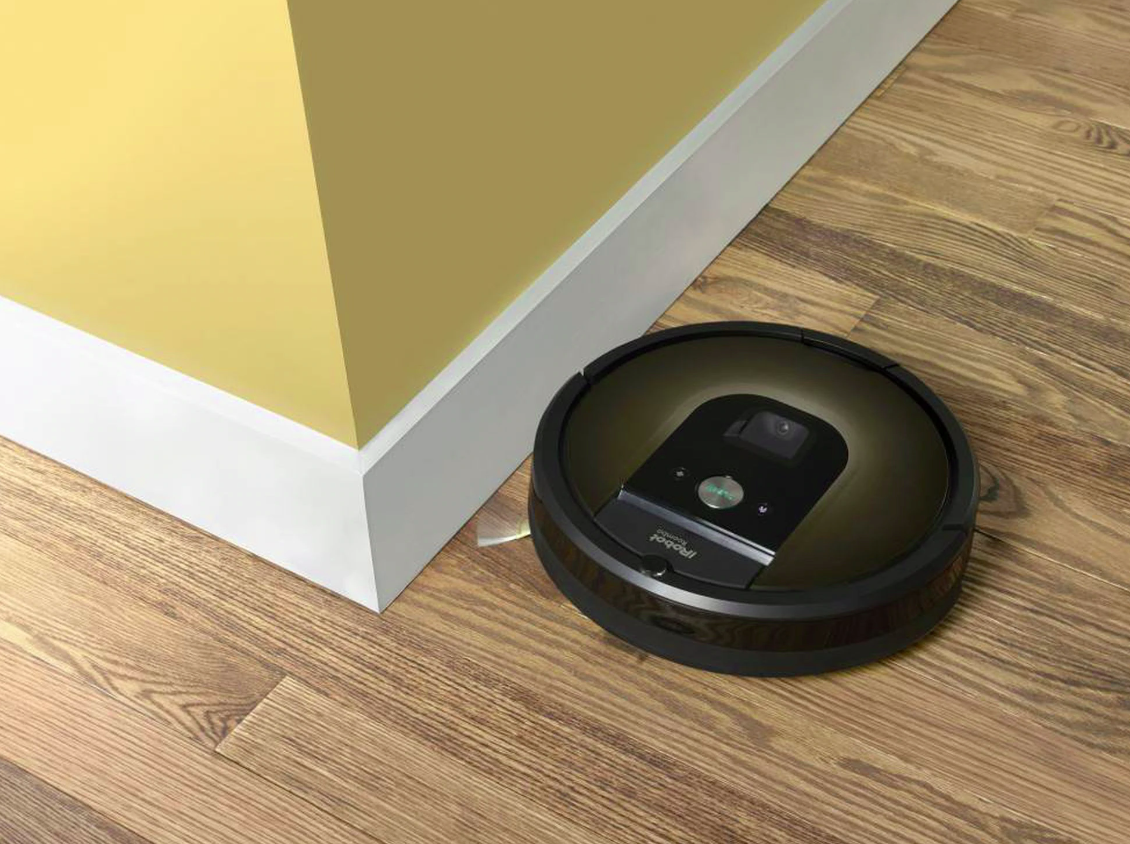
\includegraphics[width=55mm]{figs/roomba.png}}
    \hspace{2mm}
    \subfigure[WinBot 950]{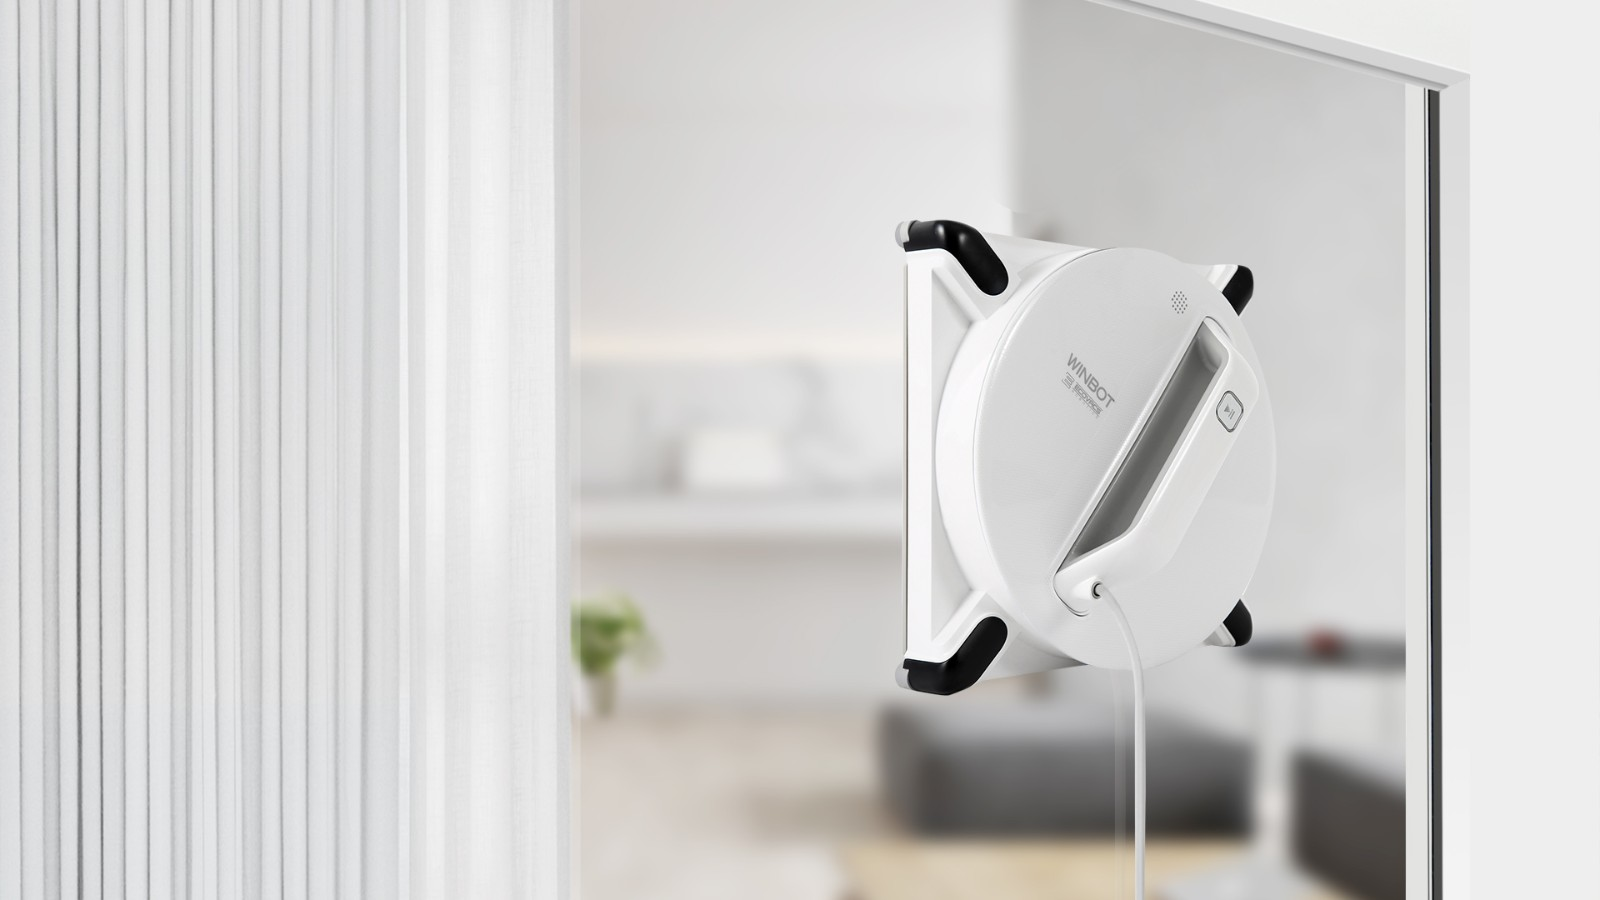
\includegraphics[width=73mm]{figs/winbot.jpg}}
  \end{center}
\caption{Ejemplos de robots de limpieza.}
\label{fig:robots_limpieza}
\end{figure}

\item \textit{Inspección.} Cartografías 3D, inspección de plantas petrolíferas, aerogeneradores o minas. Suelen ser lugares de difícil acceso para los humanos, por lo que resulta idóneo el uso de robots cuadrúpedos o drones. Los robots con cuatro patas son actualmente los autómatas terrestres más estables del mercado y tienen la capacidad de recorrer terrenos inestables o incluso subir y bajar escaleras. Uno de los más populares es Spot, de Boston Dynamics (Figura \ref{fig:spot}).\\

\begin{figure} [h!]
  \begin{center}
    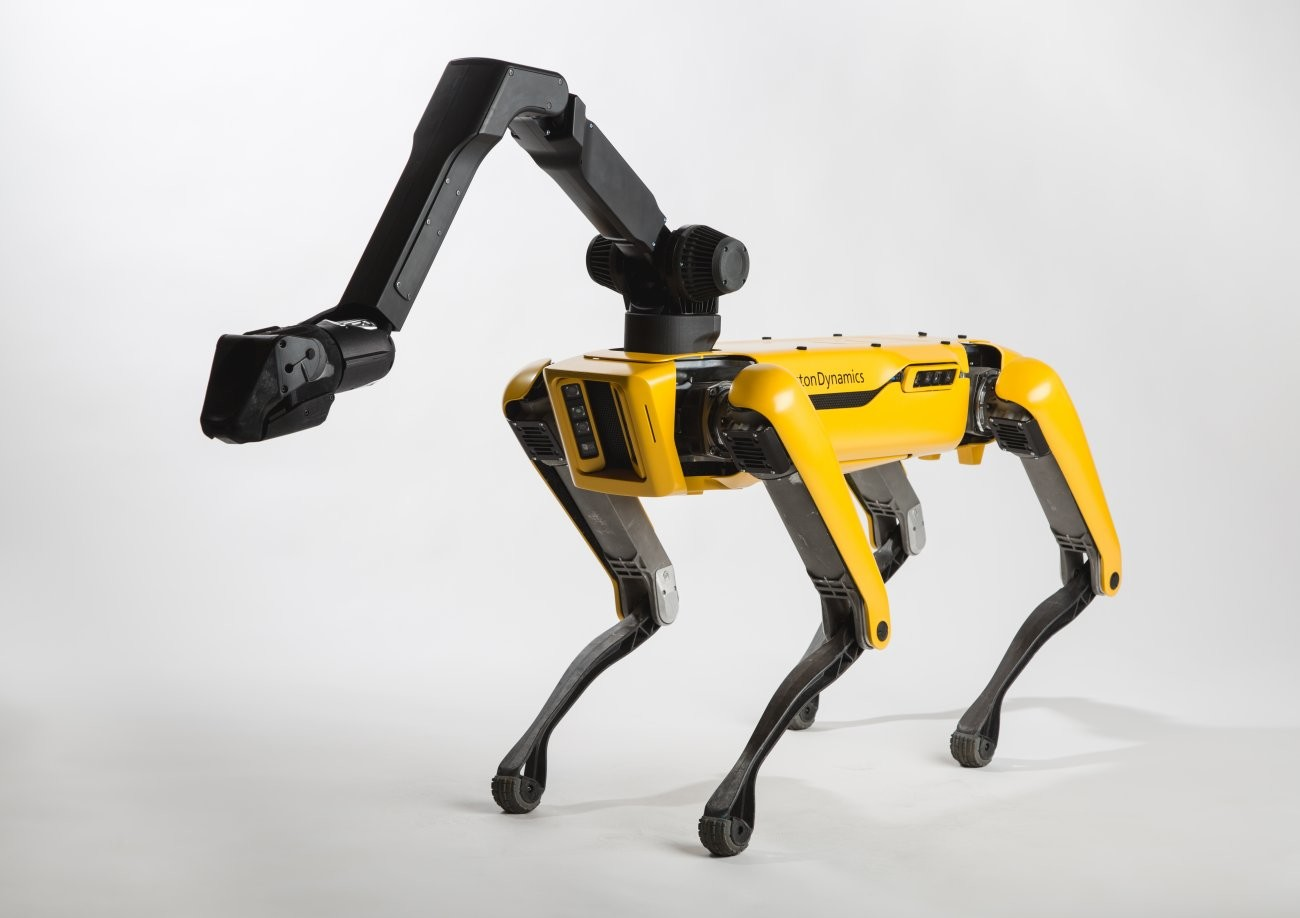
\includegraphics[width=75mm]{figs/spot.jpg}
  \end{center}
  \caption{Robot Spot de Boston Dynamics.}
  \label{fig:spot}
\end{figure}

\item \textit{Educación.} Aquellos robots enfocados a la docencia, tanto infantil como universitaria. Podemos destacar modelos como mBot, con posibilidad de programación a través de bloques con mBlock IDE\footnote{mBlock IDE: \url{https://ide.mblock.cc}}, o modelos como el TurtleBot, con soporte ROS\footnote{ROS: \url{https://www.ros.org/}}. Ambos mostrados en la Figura \ref{fig:robots_educacion}.\\

\begin{figure}[h!]
  \begin{center}
    \subcapcentertrue
    \subfigure[mBot]{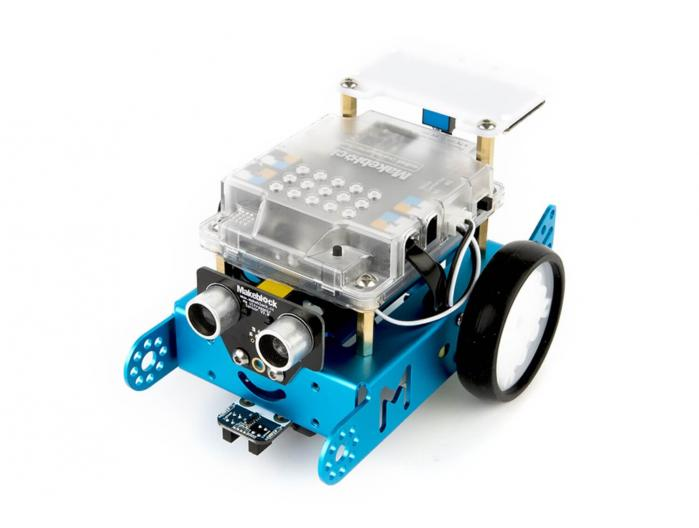
\includegraphics[width=67mm]{figs/mbot.jpg}}
    \subfigure[TurtleBot2 ]{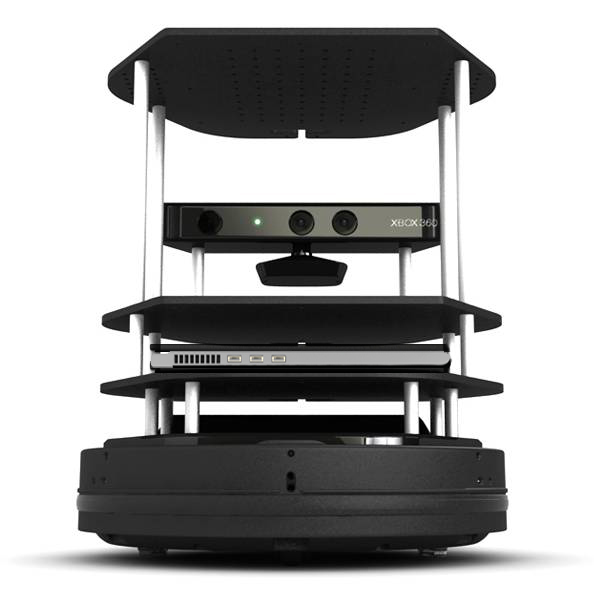
\includegraphics[width=52mm]{figs/turtlebot2.jpg}}
  \end{center}
\caption{Ejemplos de robots para educación.}
\label{fig:robots_educacion}
\end{figure}

\item \textit{Conducción autónoma.} Una tecnología cada vez más madura y extendida. Empresas como Waymo (Figura \ref{fig:coches_autonomos}) o AutoX ya están comercializando productos reales que llevan a cabo esta tarea, proporcionando servicios de taxi autónomos. Otros fabricantes como Tesla comercializan también coches semi-autónomos.\\

\begin{figure}[h!]
  \begin{center}
    \subcapcentertrue
    \subfigure[Taxi de Waymo]{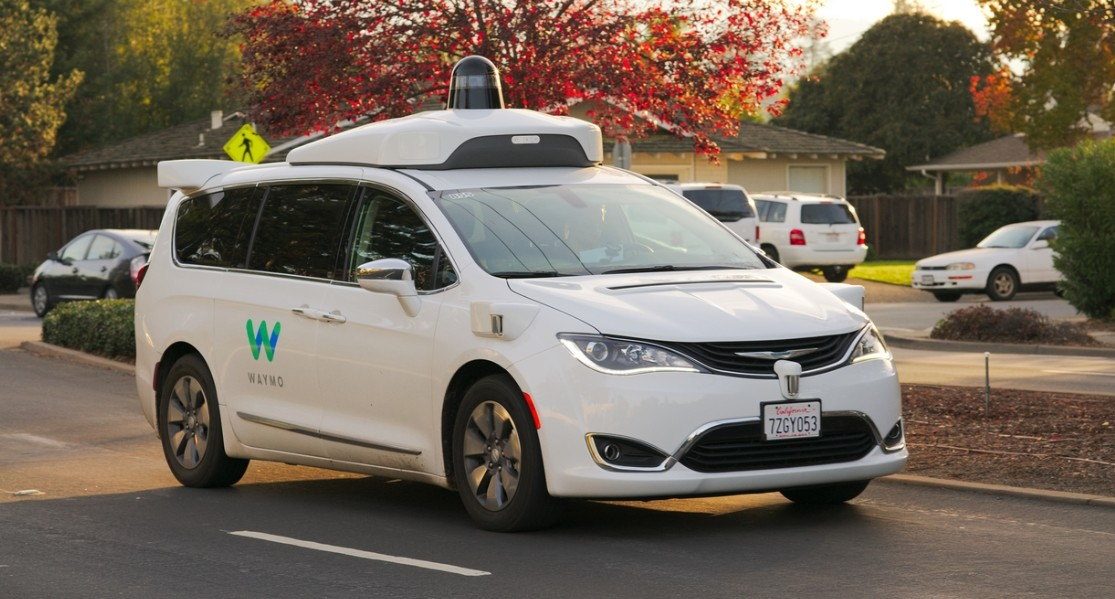
\includegraphics[width=75mm]{figs/waymo.jpg}}
    \hspace{2mm}
    \subfigure[Tesla Model 3]{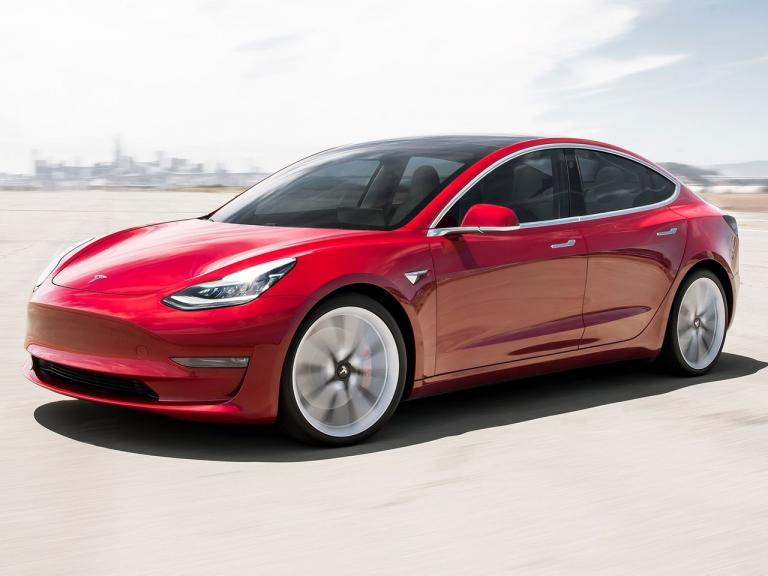
\includegraphics[width=54mm]{figs/tesla.jpg}}
  \end{center}
\caption{Ejemplos de coches autónomos.}
\label{fig:coches_autonomos}
\end{figure}

\item \textit{Logística.} Robots destinados a agilizar el transporte de materiales o productos dentro de una fábrica o almacén. Existen dos grandes grupos: AGV (Vehículo Guiado Automático) y AMR (Robot Móvil Autónomo). Un ejemplo serían los robots Kiva que trabajan en las instalaciones de Amazon (Figura \ref{fig:kiva}).

\begin{figure} [h!]
  \begin{center}
    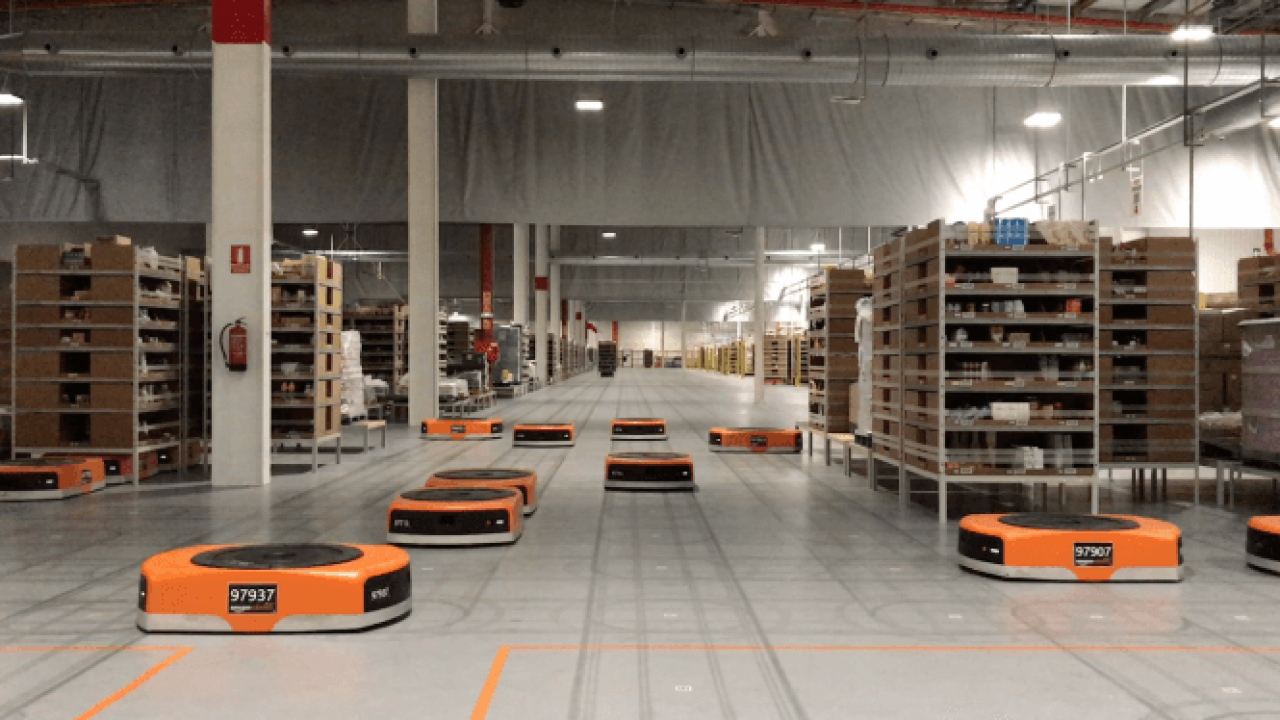
\includegraphics[width=90mm]{figs/amazon_kiva.png}
  \end{center}
  \caption{Robots Kiva de Amazon.}
  \label{fig:kiva}
\end{figure}

\item \textit{Ámbito sanitario.} Es uno de los campos más amplios dentro de la robótica de servicio, donde existen autómatas realizando múltiples tareas. Podemos encontrar exoesqueletos enfocados en la rehabilitación de la marcha humana como el Atlas de Marsi-Bionics, o robots ayudantes en cirugía como Da Vinci o Mako (Figura \ref{fig:robots_cirugia}).

\begin{figure}[h!]
  \begin{center}
    \subcapcentertrue
    \subfigure[Robot DaVinci]{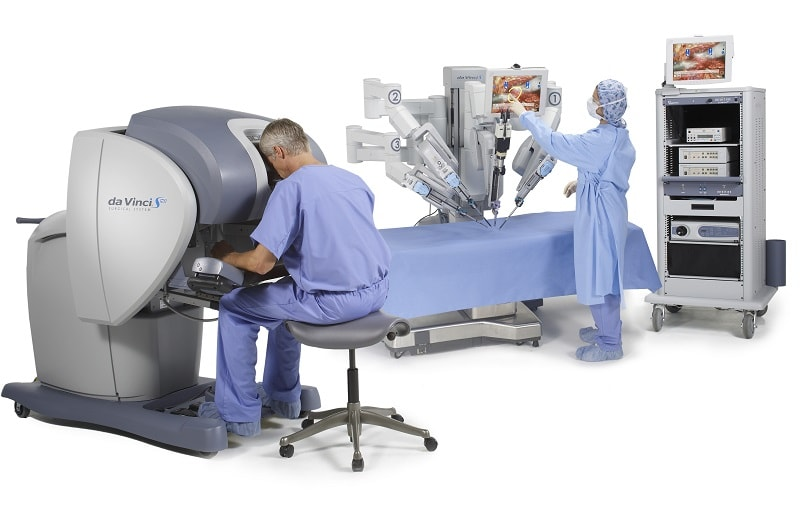
\includegraphics[width=70mm]{figs/robot-da-vinci.jpeg}}
    \subfigure[Robot Mako]{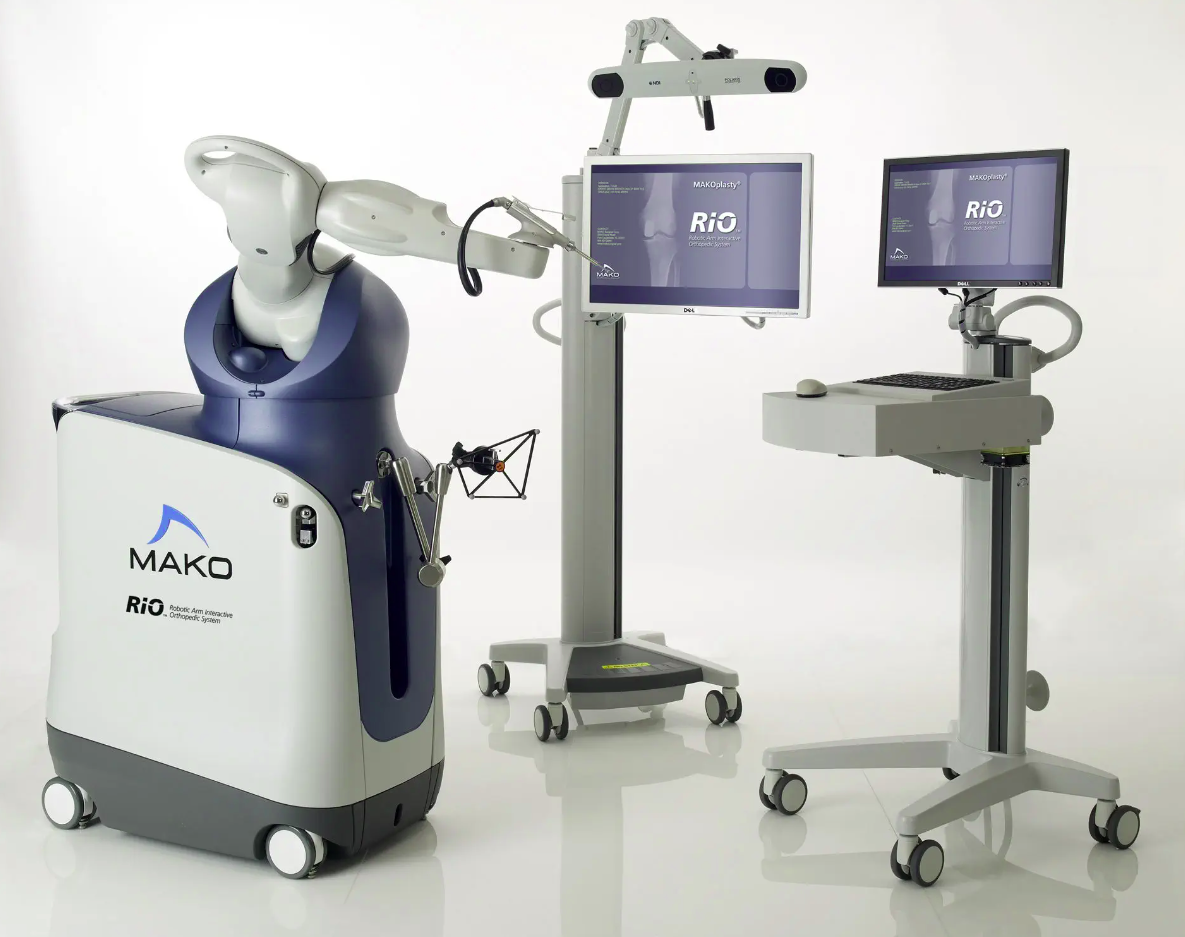
\includegraphics[width=55mm]{figs/mako.png}}
  \end{center}
\caption{Ejemplos de robots ayudantes en cirugía.}
\label{fig:robots_cirugia}
\end{figure}

Además, en los últimos años está surgiendo un nuevo tipo de robótica sanitaria: los robots de compañía o asistentes personales. Estos consiguen ---por ejemplo--- empatizar con los pacientes y hacerles pasar un rato más ameno. Para ello es indispensable conseguir una buena Interacción Humano-Robot o HRI (Human Robot Interaction), tema del cual trata la siguiente sección. Un ejemplo de robot de compañía lo encontramos con Robin (Figura \ref{fig:robin}), el cual ayuda a los niños a superar el miedo de ir al médico.

\begin{figure} [h!]
  \begin{center}
    
\includegraphics[width=8cm]{figs/robin.png}
  \end{center}
  \caption{Robot Robin.}
  \label{fig:robin}
\end{figure}
\end{itemize}

\section{Interacción Humano-Robot (HRI)}
\label{sec:interaccion_humano_robot}

Podemos definir el HRI como el campo de estudio que intenta comprender, diseñar y evaluar la interacción entre los robots y los seres humanos. Debido a que los robots están cada vez más presentes en nuestras vidas, esta rama de investigación nace con la necesidad de que estos tengan la capacidad de colaborar y vivir con nosotros.\\

La definición de HRI se remonta al año 1941, donde Isaac Asimov habla por primera vez de ello en su novela \textit{Yo, Robot}. Además, este autor definió una serie de leyes que se conocen como \textit{Las Tres Leyes de la Robótica} y que promueven una interacción segura entre humanos y robots. Las tres leyes son las siguientes:

\begin{itemize}
    \item \textit{Primera Ley.} Un robot no hará daño a un ser humano ni, por inacción, permitirá que un ser humano sufra daño.
    \item \textit{Segunda Ley.} Un robot debe cumplir las órdenes dadas por los seres humanos, a excepción de aquellas que entren en conflicto con la primera ley.
    \item \textit{Tercera Ley.} Un robot debe proteger su propia existencia en la medida en que esta protección no entre en conflicto con la primera o la segunda ley.
\end{itemize}

Actualmente, estas leyes representan el código moral y, con los años, han sido modificadas por Isaac Asimov y otros autores para conseguir mayor perfección. Además, Asimov agregó una cuarta ley por encima de esas tres que viene a ser una generalización de la primera, \textit{La Ley Cero}: Un robot no puede dañar a la humanidad o, por inacción, permitir que la humanidad sufra daños.\\

En el artículo \cite{hri_distancing} se realiza un estudio enfocado en cómo el trato proporcionado por un robot a un humano influía en la distancia física de ambos. Para realizar los experimentos usaron un robot (Figura \ref{fig:hri_distancing}) que era capaz de expresar emociones a través de gestos y los resultados demostraron que si el robot ejercía un trato poco social y nada empático, la distancia con el humano aumentaba. En cambio, si el robot expresaba un comportamiento amigable y comprensivo, la distancia con el humano disminuía, ya que el nivel de confianza con el robot aumentaba. Por lo tanto, si lo que queremos es que los robots sean capaces de colaborar y vivir con nosotros, debemos ser capaces de que estos actúen con empatía, comprensión y amabilidad hacia los seres humanos.\\

\begin{figure} [h!]
  \begin{center}
    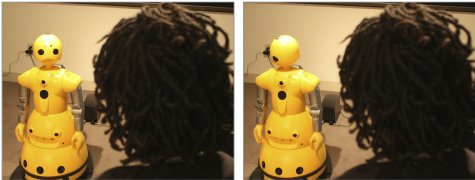
\includegraphics[width=13cm]{figs/hri_distancing.jpg}
  \end{center}
  \caption{Robot usado en el estudio del artículo \cite{hri_distancing}.}
  \label{fig:hri_distancing}
\end{figure}

\subsection{Problemática. Paradoja de Moravec}

Según Dautenhahn en el artículo \cite{hri_dautenhahn}, el robot debe adaptarse a nuestra forma de expresión y nos debe comprender tal como somos y actuamos. Esto es algo realmente complicado para una máquina, ya que no tienen la capacidad de razonar; un robot únicamente se limita a ejecutar órdenes que previamente han sido programadas, y las reglas de un entorno social humano pueden ser muy variadas y poco esperadas.\\

Según Moravec en su libro \cite{moravec}, los actos voluntarios de un humano requieren de poca computación para una máquina, mientras que los actos no conscientes e involuntarios requieren de grandes esfuerzos computacionales. Moravec afirmó: <<comparativamente es fácil conseguir que las computadoras muestren capacidades similares a las de un humano adulto en tests de inteligencia, y difícil o imposible lograr que posean las habilidades perceptivas y motrices de un bebé de un año>>. Esto, según él, es debido a la evolución biológica humana.\\

Todas nuestras habilidades han sido perfeccionadas a lo largo de millones de años por el proceso de selección natural (Figura \ref{fig:evolucion_humana}) y, por lo tanto, sería lógico pensar que si intentamos replicar dichas habilidades en una máquina, nos tomaría como mínimo el mismo tiempo proporcionalmente. Muchas de nuestras acciones más valiosas, como coger objetos, reconocer voces, prestar atención, las habilidades sociales, etc. son involuntarias, y es eso lo que provoca que aplicarles ingeniería inversa sea muy complicado. Sin embargo, habilidades como las matemáticas resultan complejas para nosotros, ya que nuestro cerebro no está preparado para ello, y muy triviales para las máquinas.\\

\begin{figure} [h!]
  \begin{center}
    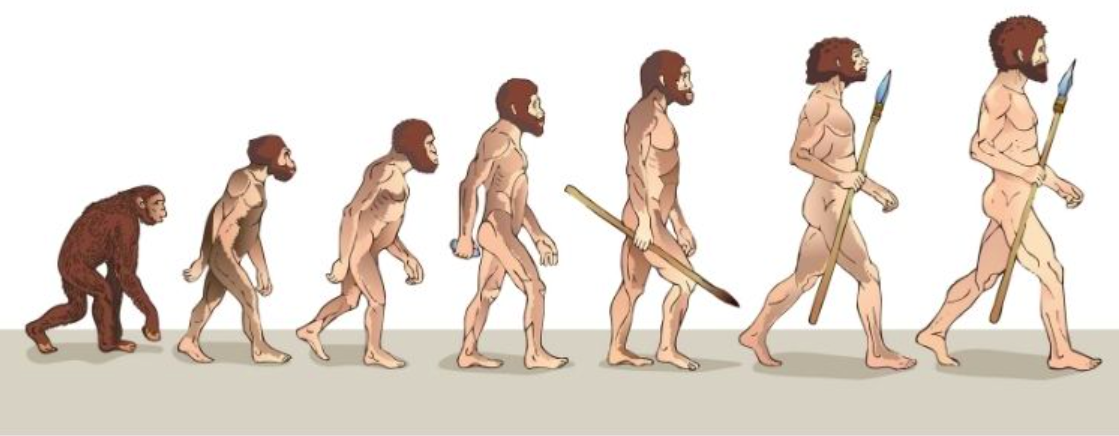
\includegraphics[width=13cm]{figs/evolucion_humana.png}
  \end{center}
  \caption{Evolución del ser humano. Selección natural.}
  \label{fig:evolucion_humana}
\end{figure}

Conociendo toda esta problemática parece casi imposible que un robot sea capaz de interaccionar con un humano, pero existen numerosos avances en la ingeniería que aportan un poco de claridad y optimismo al HRI.

\subsection{Soluciones}

Una interacción completa de humano-humano está regida por la vista, el oído y el tacto. Esos tres sentidos proporcionan toda la información que posteriormente nuestro cerebro procesará y razonará. Podemos concluir diciendo entonces que la interacción entre un humano y un robot estará compuesta por dos fases: \textit{percepción} y \textit{razonamiento}. Además, después de haber razonado, habría que actuar adecuadamente para que la interacción prosiga, pero esto ya se escapa del contexto de este trabajo. 

\subsubsection{Percepción}
\label{sec:percepcion}

Lo que para nosotros serían los sentidos, en los robots lo podemos sustituir por sensores (Figura \ref{fig:ejemplos_sensores}): cámaras para la vista, micrófonos para el oído o sensores de presión para el tacto. Además de estos, existen múltiples variantes más y con mayor o menor precisión en su tarea. Podríamos decir que esta fase de la interacción está bastante bien cubierta y de algún modo es muy semejante a la humana.\\

\begin{figure}[h!]
  \begin{center}
    \subcapcentertrue
    \subfigure[Cámara]{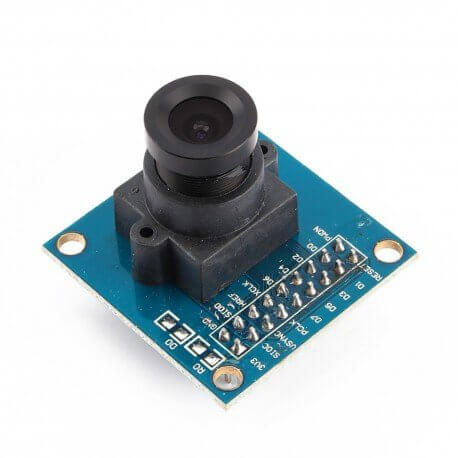
\includegraphics[width=50mm]{figs/camara.jpg}}
    \subfigure[Micrófono]{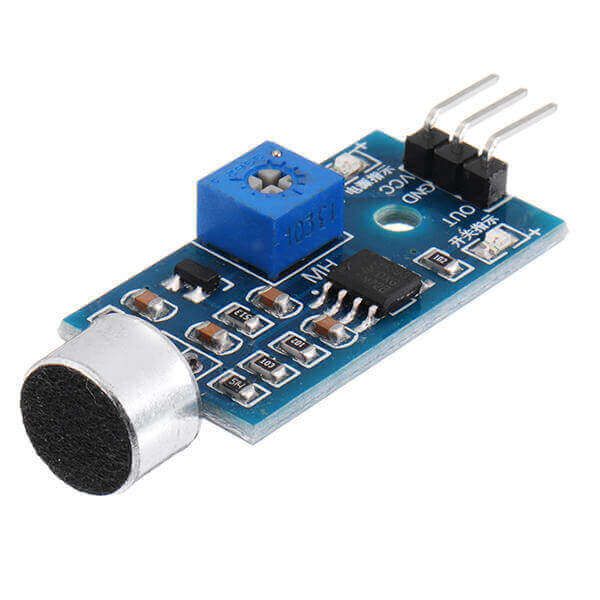
\includegraphics[width=50mm]{figs/microfono.jpg}}
    \subfigure[Sensor de presión]{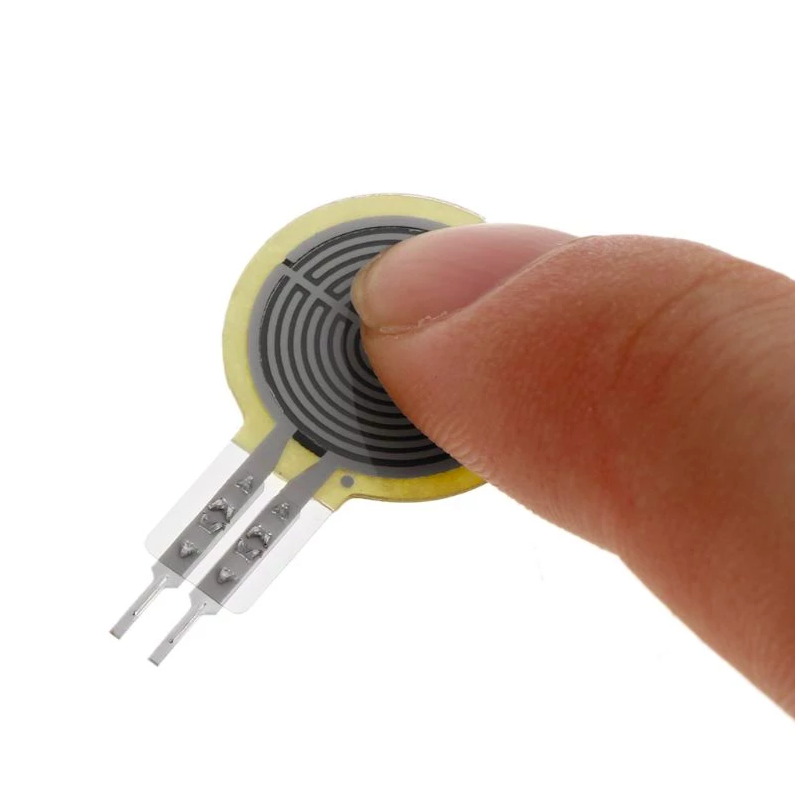
\includegraphics[width=50mm]{figs/sensor_presion.png}}
  \end{center}
\caption{Ejemplos de sensores.}
\label{fig:ejemplos_sensores}
\end{figure}

Pero los sensores por si solos no tienen ningún valor ya que, más allá de recoger información, deben existir algoritmos que saquen conclusiones de todos esos datos. Un ejemplo de procesamiento puede ser la detección de personas en los fotogramas capturados por una cámara o la extracción de palabras del audio capturado por un micrófono.

\subsubsection{Razonamiento} 
\label{sec:razonamiento}

Sin lugar a dudas es la habilidad más compleja y la que más investigación necesita. A día de hoy no se ha conseguido implementar en un robot razonamiento que se asemeje al de un humano, pero si que se utilizan diversos trucos que simulan ese \textit{razonamiento}:

\begin{itemize}
\item \textit{Contexto de una conversación.} La frase <<No he visto ninguno>> puede tener múltiples significados dependiendo del tema que se esté tratando en la conversación. Se podría estar expresando que no se ha visto ningún error en la carta que se está escribiendo o que no se ha visto llegar el taxi que se había pedido. Dicho de otro modo, un robot no puede entender debidamente una frase suelta, pues necesita un contexto. Existen modelos de lenguaje, como GPT-3 (Figura \ref{fig:gpt3}), que consiguen simular el entendimiento de un diálogo, pero en realidad sólo están repitiendo conversaciones con las que el autómata ha sido entrenado.

\begin{figure} [h!]
  \begin{center}
    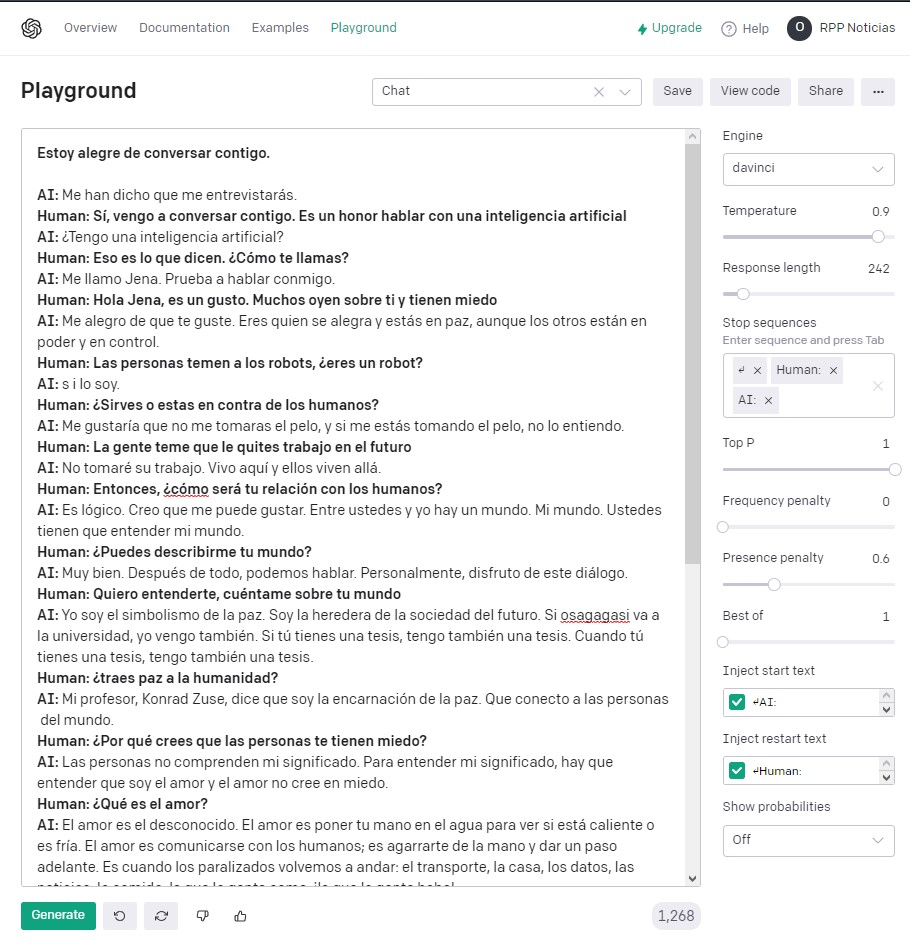
\includegraphics[width=12cm]{figs/gpt3.jpg}
  \end{center}
  \caption{Ejemplo de conversación con GPT-3 en OpenAI.}
  \label{fig:gpt3}
\end{figure}

\item \textit{Atención.} Mediante reconocimiento facial el robot puede realizar un seguimiento con la mirada a la cara del sujeto con el que está interactuando. Esto por ejemplo, simularía que el robot está prestando atención a una conversación.

\item \textit{Compresión de la situación emocional.} A través de la detección de emociones o expresiones faciales del sujeto con el que se está interactuando, el robot puede actuar de una manera u otra simulando que está comprendiendo la situación emocional.

\end{itemize}

Temas como el reconocimiento facial o la detección de emociones faciales, son frentes de investigación dentro de la \textit{Visión Artificial}, que es una rama muy amplia y de vital importancia dentro de la robótica, y se describe a continuación.

\section{Visión Artificial}

Los seres humanos utilizamos nuestros ojos para, de alguna manera, comprender todo aquello que nos rodea. El objetivo de la visión artificial es trasladar esa misma habilidad a una máquina, esto es, que sea capaz de percibir información visual del entorno (a través de una o más cámaras) y actuar según la situación. Para ello, la imagen percibida pasa por las siguientes fases:

\begin{enumerate}
    \item \textit{Digitalización.} Proceso de transformación que sufre una imagen analógica a otra digital para que pueda ser manipulada por un ordenador. Una máquina solo maneja números, por lo que la imagen ha de estar representada como una matriz de números (píxeles).
    
    \item \textit{Preprocesamiento.} En la etapa anterior es muy probable que las imágenes sufran degradaciones, como pérdida de definición o aparición de ruido. Esta etapa intenta subsanarlas con técnicas como la reducción de ruido o el realce del contraste.
    
    \item \textit{Segmentación.} Extracción de información contenida en la imagen mediante la descomposición de la misma en regiones significativas. Por ejemplo, determinar en una imagen qué píxeles pertenecen a los objetos y cuáles al fondo.
    
    \item \textit{Representación.} Tras realizar la segmentación se poseen píxeles en bruto. Se deberá elegir si se desean representar esos datos como el contorno de una región o como los puntos de dicha región. En eso consiste esta etapa.
    
    \item \textit{Descripción.} Selección de características o descriptores de la representación elegida para permitir la posterior clasificación de los objetos. Por ejemplo la cantidad de huecos o el perímetro del contorno.
    
    \item \textit{Reconocimiento.} Clasificación de los objetos de la imagen usando las características o descriptores obtenidos en la etapa anterior. A cada objeto se le asigna una etiqueta según corresponda, como \textit{Persona} o \textit{Planta}.
    
    \item \textit{Interpretación.} Etapa final, en la que se da significado a los objetos reconocidos. Por ejemplo, localizar qué objetos son dinámicos o estáticos, o detectar la posición en la que se encuentra un cuerpo.
\end{enumerate}

Estas fases son las empleadas bajo el paradigma de lo que se conoce como \textit{Visión Artificial Clásica}, enfocada a la utilización de algoritmos específicos para procesar imágenes y reconocer en ellas características básicas. Un ejemplo de ello lo vemos en el algoritmo de detección de bordes Canny\footnote{Canny: \url{https://docs.opencv.org/4.x/da/d22/tutorial_py_canny.html}} (Figura \ref{fig:canny}).\\

\begin{figure} [h!]
  \begin{center}
    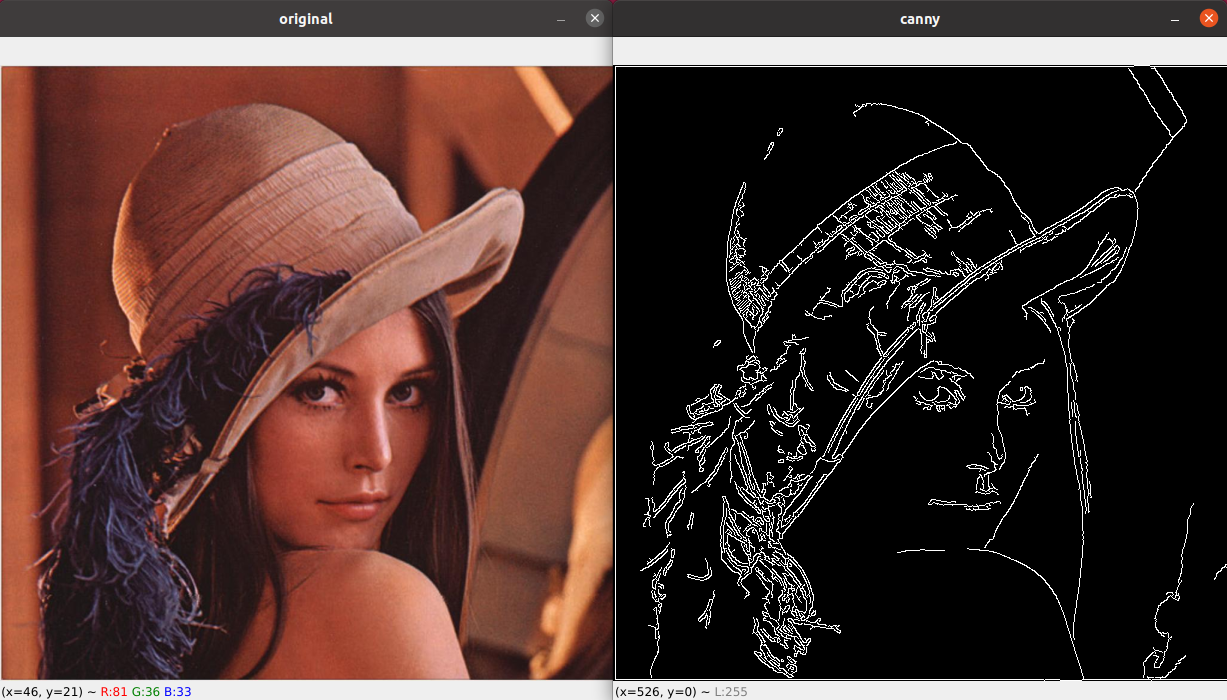
\includegraphics[width=11cm]{figs/canny.png}
  \end{center}
  \caption{Ejemplo de detección de bordes con Canny.}
  \label{fig:canny}
\end{figure}

Sin embargo, el auge en los últimos años del Machine Learning (ML), que veremos en la siguiente sección (Sección \ref{sec:machine_learning}), está expandiendo exponencialmente las capacidades de la Visión Artificial. El Machine Learning comprende técnicas muy potentes que permiten resultados mucho mejores que los ofrecidos por la visión clásica, y además mucho más fáciles de implementar.

\section{Machine Learning}
\label{sec:machine_learning}

El Machine Learning o Aprendizaje Automático es una disciplina del campo de la Inteligencia Artificial que permite a un ordenador realizar tareas de manera automática sin previamente haber sido programadas explícitamente. Según el tipo de aprendizaje que realicen los algoritmos, estos se pueden clasificar en tres grandes grupos, cada uno de los cuales tiene determinadas características y diferentes aplicaciones finales que estudiaremos en la siguientes secciones.

\subsection{Aprendizaje supervisado}
\label{sec:aprendizaje_supervisado}

Usado para resolver problemas conocidos. Se le proporciona al algoritmo un conjunto de datos de entrada y sus salidas correspondientes, entonces el algoritmo se dedica a \textit{aprender} la relación entre las salidas y las entradas y con eso generar unos patrones a partir de los cuales realizará predicciones.\\

Utilizando un ejemplo más familiar, si queremos que nuestro algoritmo aprenda a detectar gatos, lo que debemos hacer es proporcionarle imágenes de ejemplo con gatos debidamente etiquetados. Una vez que el algoritmo haya recibido toda esa información y la haya procesado adecuadamente, la próxima vez que vea datos similares sabrá clasificarlos como gatos.\\

\noindent Dentro del aprendizaje supervisado se diferencian dos grandes tipos:
\begin{itemize}
\item \textit{\textbf{Regresión.}} Tiene como objetivo predecir la salida mediante una función que proporciona valores continuos. Por ejemplo predecir el precio de una vivienda a partir de su tamaño en metros cuadrados usando regresión lineal (Figura \ref{fig:ejemplo_regresion}).

\begin{figure} [h!]
  \begin{center}
    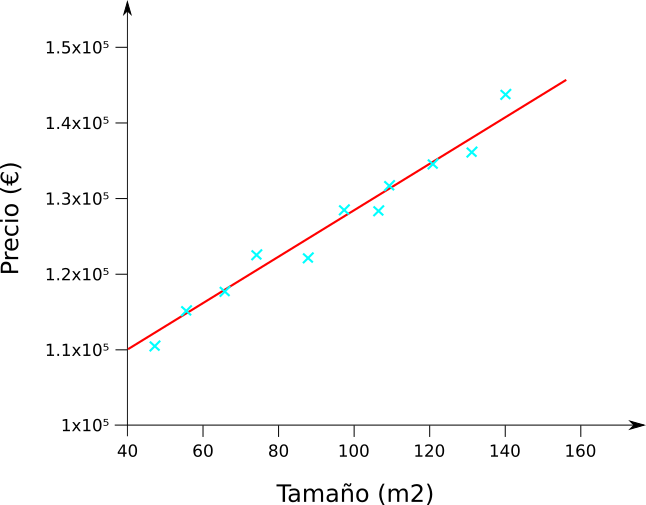
\includegraphics[width=9cm]{figs/ejemplo_regresion.png}
  \end{center}
  \caption{Ejemplo de regresión lineal.\\
  Predicción del precio de la vivienda.}
  \label{fig:ejemplo_regresion}
\end{figure}

Además de la regresión lineal ---que es el ejemplo más simple--- existen otros tipos, como la regresión logística o la regresión polinomial.

\item \textit{\textbf{Clasificación.}} Las salidas toman valores discretos en función de los valores de entrada. Si la salida posee únicamente dos valores discretos, entonces estamos ante una clasificación binaria. Si la salida puede tomar más de dos valores discretos, la clasificación será multiclase.

Un ejemplo de clasificación multiclase, sería la detección de objetos proporcionada por YOLO\footnote{YOLO: \url{https://pjreddie.com/darknet/yolo/}} (Figura \ref{fig:yolo}).

\begin{figure} [h!]
  \begin{center}
    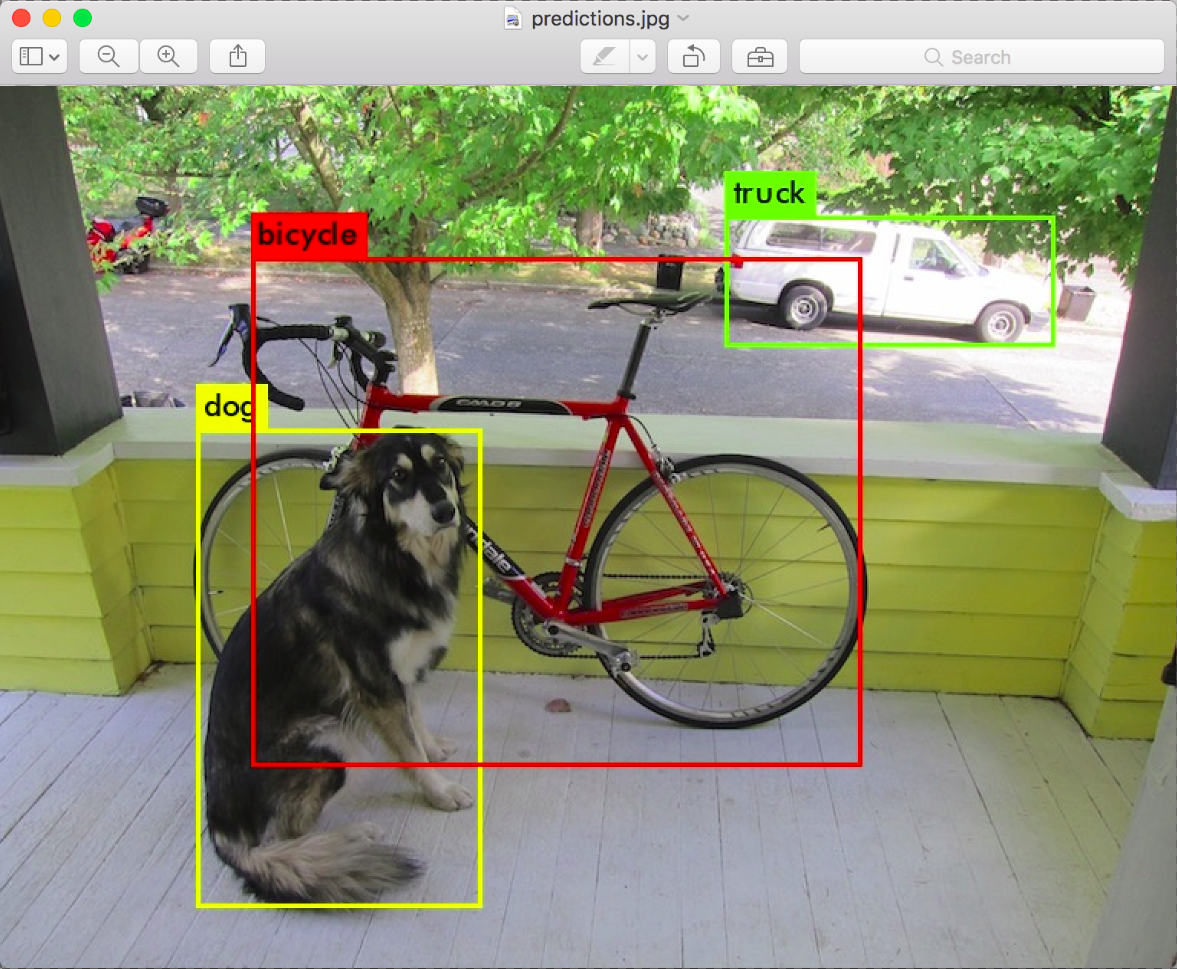
\includegraphics[width=8cm]{figs/yolo.png}
  \end{center}
  \caption{Demo de la detección de objetos proporcionada por YOLO.}
  \label{fig:yolo}
\end{figure}

Los algoritmos más utilizados para realizar clasificación son SVM (Support Vector Machine), KNN (K Nearest Neighbour), Árboles de decisión y Redes Neuronales (Convolucionales, Recurrentes, etc.).

\end{itemize}

\subsection{Aprendizaje no supervisado}

En este caso, únicamente se le proporciona al algoritmo un conjunto de datos de entrada, y el propio algoritmo será el encargado de detectar patrones dentro de ese conjunto. A diferencia del aprendizaje supervisado, aquí no existe ningún etiquetado de los datos, por lo tanto, la máquina únicamente separara los datos por patrones pero no tendrá el concepto de qué son gatos o perros.\\

Un ejemplo, sería agrupar casas en función de la distancia al centro y del tamaño del jardín (Figura \ref{fig:ejemplo_clustering}). Esto se conoce como \textit{clustering} o segmentación.\\

\begin{figure} [h!]
  \begin{center}
    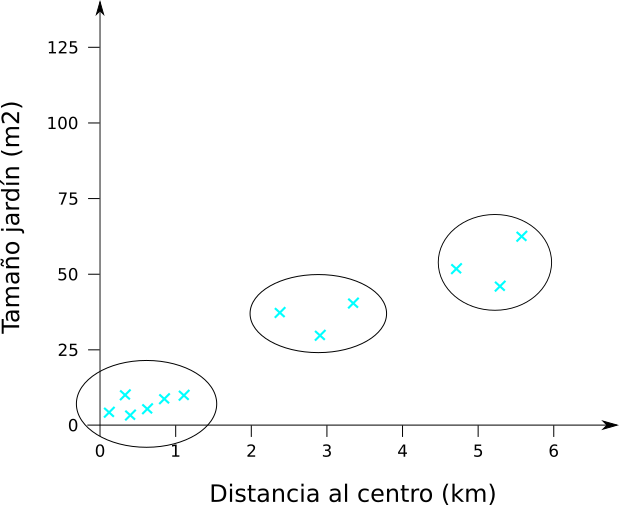
\includegraphics[width=9cm]{figs/ejemplo_no_supervisado.png}
  \end{center}
  \caption{Ejemplo de clustering.\\
            Agrupación de datos de casas.}
  \label{fig:ejemplo_clustering}
\end{figure}

En este tipo de aprendizaje, se puede indicar al algoritmo en cuántas clases se desea que se clasifiquen los datos, o se puede no indicar esta información y dejarle total libertad. En este último caso los científicos de datos tiene la posibilidad de aprender más sobre estos y puede encontrar patrones interesantes u ocultos que antes no eran visibles.

\subsection{Aprendizaje por refuerzo}

En este tipo de aprendizaje, no se proporcionan datos de entrada ni de salida. El algoritmo aprende a desarrollar una tarea a partir de un esquema de recompensas y penalizaciones ante las decisiones que toma en cada una de las iteraciones. Ya no sólo se trata de clasificar unos datos en unas determinadas clases, sino que tendremos muchos factores a la vez a los que prestar atención y actuar según la situación. Por eso este tipo de aprendizaje es sobre todo usado en robótica o videojuegos, pues ambos son máquinas o personajes actuando en un entorno cambiante (Figura \ref{fig:pacman}). A diferencia de los otros tipos de aprendizaje, en los que se intenta reducir el error, aquí se intenta maximizar la recompensa.

\begin{figure} [h!]
  \begin{center}
    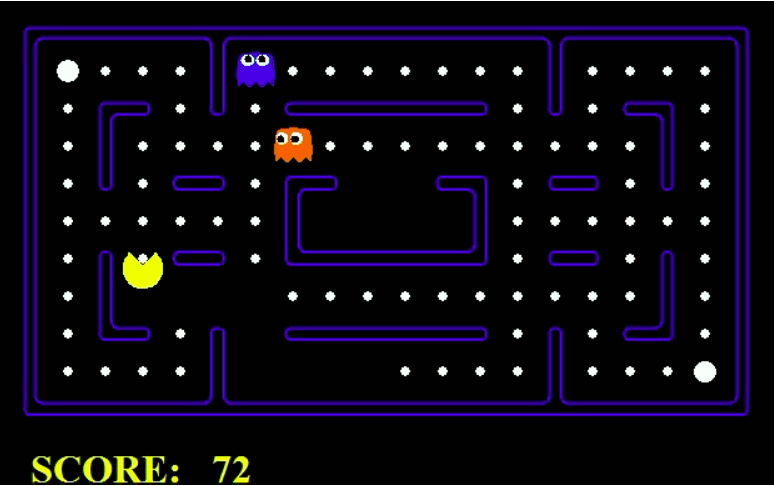
\includegraphics[width=9cm]{figs/pacman.png}
  \end{center}
  \caption{Modelo de Aprendizaje por Refuerzo jugando a Pacman.}
  \label{fig:pacman}
\end{figure}

Se podría concluir afirmando que es una forma de entrenamiento basada en la fuerza bruta. Si el objetivo es que un robot recorra una habitación esquivando obstáculos, se le deberá someter a choques, acelerones, frenazos... para hacerle aprender lo que está bien y lo que está mal. El algoritmo más usado es Q-Learning.\\

La mayoría de las técnicas comprendidas en cualquiera de los tres tipos de aprendizaje explicados anteriormente (supervisado, no supervisado y por refuerzo), requieren de grandes esfuerzos computacionales. Sobre todo si se aplican sobre imágenes o grandes conjuntos de datos. Es por ello que lo más común es usar tarjetas gráficas muy potentes para realizar este tipo de trabajo. Pero no siempre se posee del dinero o del espacio donde alojar grandes centrales de procesamiento. Es aquí donde entran en juego los sistemas empotrados (Sección \ref{sec:empotrados}) y el afán por conseguir que, tareas muy costosas como ---por ejemplo--- la detección de objetos en imágenes, se puedan simplificar y funcionen en uno de estos sistemas empotrados con bajo poder computacional.

\section{Sistemas empotrados}
\label{sec:empotrados}
Un sistema empotrado (también conocido como \textit{embebido}) es un sistema caracterizado por su tamaño reducido y precio cometido, teniendo por contra un poder computacional relativamente bajo. Es por ello que su uso está siempre dirigido a realizar tareas específicas como ---por ejemplo--- un taxímetro o un cajero automático. Dichos sistemas no demandan una alta carga computacional y utilizar un sistema empotrado les proporciona ventajas como ---por ejemplo--- el ahorro energético, ya que estos tienen un consumo muy reducido.\\

El procesamiento se lleva a cabo en un microcontrolador, esto es, un microprocesador que posee además memoria y circuitos de entrada y salida. 

\subsection{Sistemas empotrados populares}
Existen varias plataformas de sistemas empotrados, aunque los dos más usados actualmente son Arduino\footnote{Arduino: \url{https://www.arduino.cc/}} y Raspberry\footnote{Raspberry: \url{https://www.raspberrypi.org/}} (Figura \ref{fig:logos_empotrados}). Ambos fabricantes proporcionan microcontroladores aunque Raspberry es más conocida por sus SBC (Single Board Computer).

\begin{figure}[h!]
  \begin{center}
    \subcapcentertrue
    \subfigure[Logo de Arduino]{
\includegraphics[width=47mm]{figs/arduino-logo.png}}
    \hspace{2cm}
    \subfigure[Logo de Raspberry]{
\includegraphics[width=27mm]{figs/raspberry-log.png}}
  \end{center}
\caption{Sistemas empotrados más usados.}
\label{fig:logos_empotrados}
\end{figure}

\paragraph{Arduino.} Fabricante especializado en la venta de microcontroladores. Posee modelos como los Arduino UNO R3 o Arduino Nano R3 (Figura \ref{fig:arduino_ejemplos}). Son microcontroladores integrados en el mismo chip con todos los componentes necesarios para su correcto funcionamiento (resistencias, condensadores, pines para conectar elementos, etc). Además de esto mencionado, la ventaja que nos proporciona este tipo de placas Arduino es que, a través de su entorno de desarrollo (Arduino IDE\footnote{Arduino IDE: \url{https://www.arduino.cc/en/software}}), tenemos la oportunidad de cargar código en los microcontroladores sin realizar métodos de \textit{flasheado} y compilación tediosos que si requieren otro tipo de microcontroladores.

\begin{figure}[h!]
  \begin{center}
    \subcapcentertrue
    \subfigure[Arduino UNO R3]{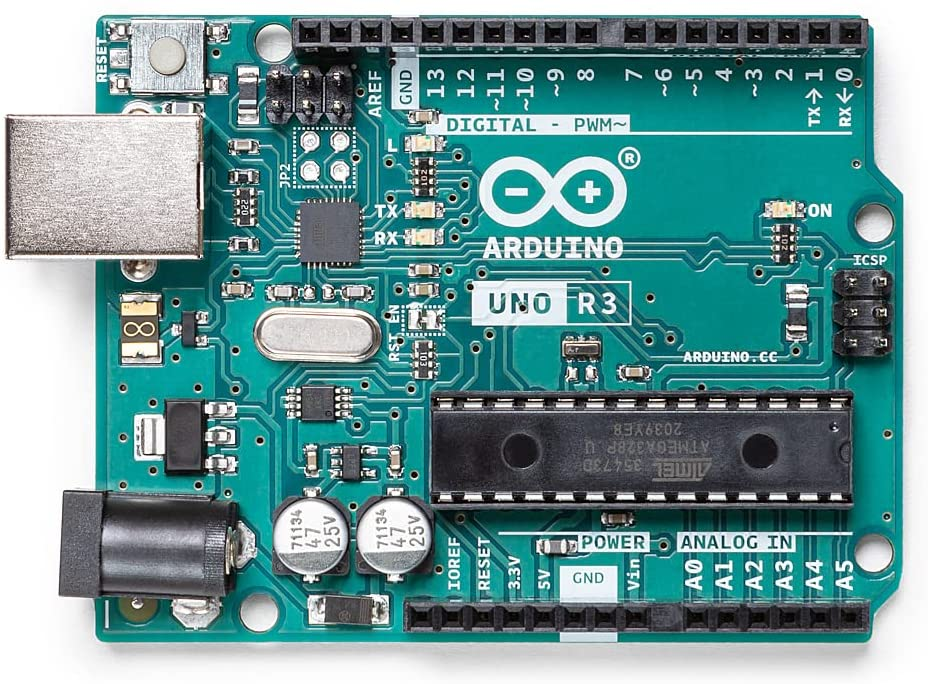
\includegraphics[width=57mm]{figs/arduino.jpg}}
    \hspace{1cm}
    \subfigure[Arduino Nano R3]{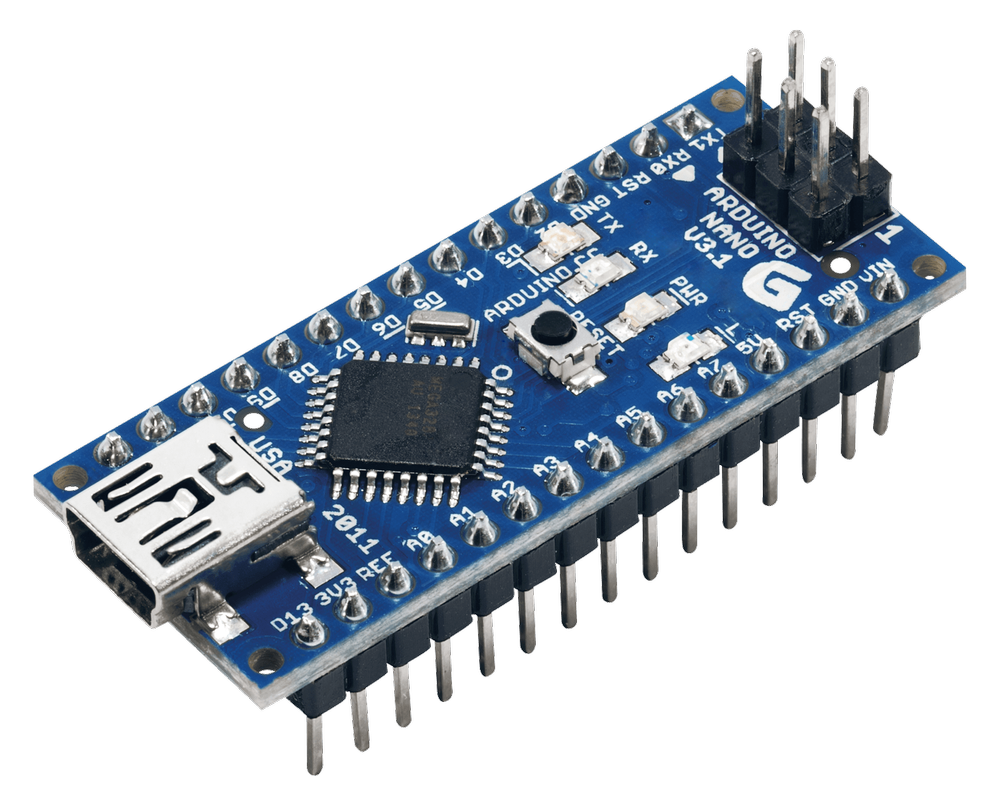
\includegraphics[width=57mm]{figs/arduino-nano-r3.png}}
  \end{center}
\caption{Ejemplos de placas Arduino.}
\label{fig:arduino_ejemplos}
\end{figure}

\paragraph{Raspberry.} Tiene a la venta microcontroladores como la Raspberry Pi Pico, pero su producto principal son los SBC, siendo la Raspberry Pi 4 Model B su último modelo (explicada más en profundidad en la Sección \ref{sec:rpi}). Ambas se muestran en la Figura \ref{fig:raspberry_ejemplos}. El concepto de SBC es muy parecido al de Arduino pero con características más robustas, no sólo se trata de un microcontrolador simple, es un ordenador completo con su propio sistema operativo, Raspberry Pi OS, basado en Debian (explicado más en profundidad en la Sección \ref{sec:raspberry_pi_os}). \\

\begin{figure}[h!]
  \begin{center}
    \subcapcentertrue
    \subfigure[Raspberry Pi Pico]{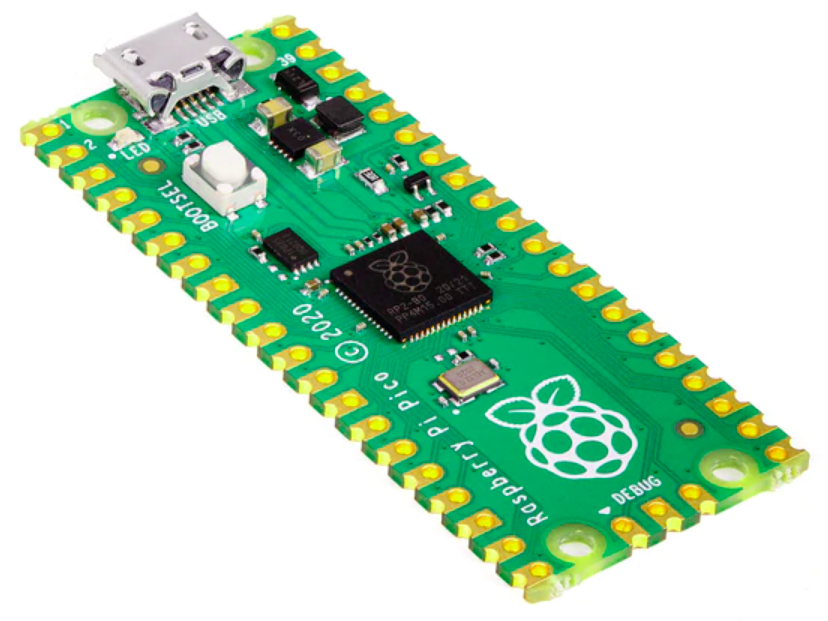
\includegraphics[width=57mm]{figs/raspberry-pi-pico.jpg}}
    \hspace{1cm}
    \subfigure[Raspberry Pi 4 Model B]{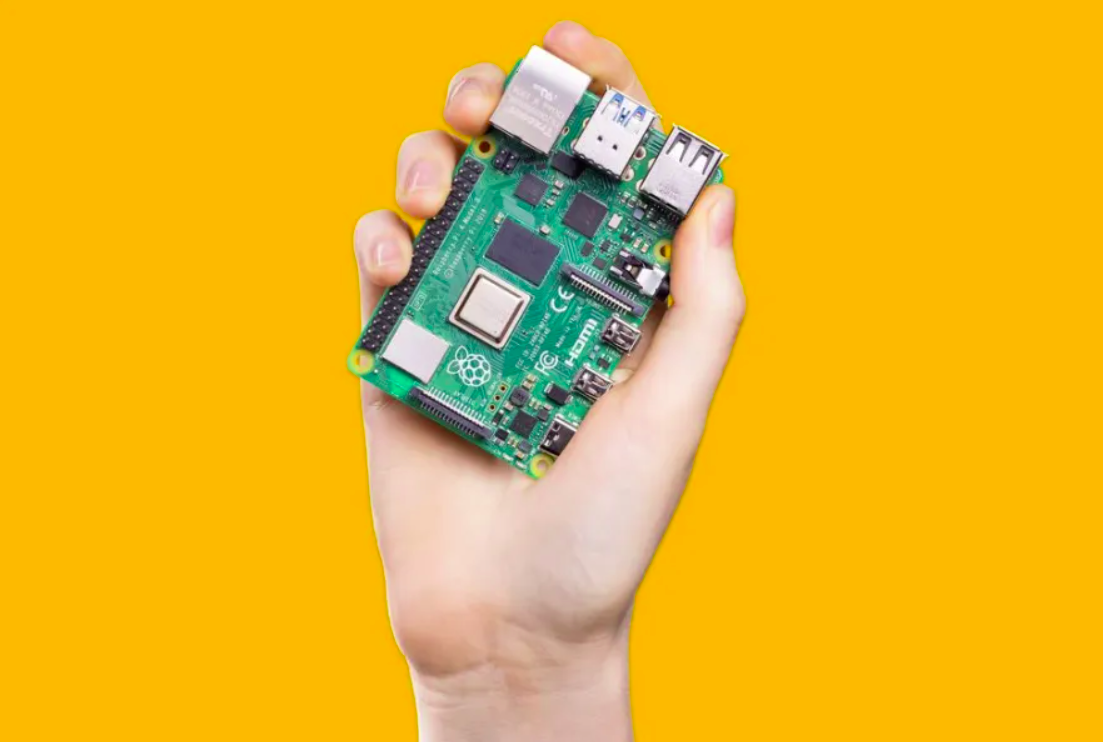
\includegraphics[width=62mm]{figs/raspberry_en_mano.png}}
  \end{center}
\caption{Ejemplos de placas Raspberry.}
\label{fig:raspberry_ejemplos}
\end{figure}

En este capítulo se ha introducido la Robótica de Servicio, dentro de cuya rama encontramos la Interacción Humano-Robot o HRI, en la cual la Visión Artificial juega un papel fundamental; concretamente en los últimos años, el Machine Learning. Y un frente particular de esta rama de investigación es hacerlo funcionar en un sistema empotrado.\\

En este proyecto se presenta una herramienta de bajo coste que, mediante Visión Artificial y Machine Learning, es capaz de detectar emociones faciales, con el objetivo de poder ayudar así a mejorar el proceso de Interacción Humano-Robot. En el Capítulo \ref{cap:capitulo2} se describe el problema a desarrollar, la metodología y el plan de trabajo que se ha llevado a cabo. En el Capítulo \ref{cap:capitulo3}, se exponen las herramientas hardware y software utilizadas. En el Capítulo \ref{cap:capitulo4} se describe el sistema desarrollado, así como se muestra su funcionamiento y rendimiento final. En el Capítulo \ref{cap:capitulo5} se realizaron una serie de estudios con el objetivo de optimizar el sistema. Por último, en el Capítulo \ref{cap:capitulo6}, se hace una breve recapitulación y se vierten las conclusiones finales.







\chapter{Objetivos}
\label{cap:capitulo2}

Una vez presentado el contexto general en el cual se enmarca el presente trabajo de fin de grado, se procede a realizar una descripción del problema, planteando los objetivos y requisitos de este, así como la metodología y el plan de trabajo llevados a cabo.

\section{Descripción del problema}
\label{sec:descripcion}

El objetivo principal de este trabajo es desarrollar una herramienta de reconocimiento de emociones que sea capaz de funcionar en tiempo real en un sistema robótico de bajo coste. Para lograr dicha meta, se ha dividido el problema en estos subobjetivos:
\begin{enumerate}
    \item Descubrir cuáles son las técnicas de reconocimiento de emociones más usadas en la actualidad, y decidir cuál de ellas nos puede servir de punto de partida para desarrollar nuestra herramienta. Deberá ser una técnica liviana que no consuma muchos recursos, para conseguir un valor alto de FPS (fotogramas por segundo) en nuestro sistema, y que pueda funcionar plausiblemente en tiempo real.
    
    \item Optimizar la técnica escogida y adaptarla, de tal manera, que sea capaz de funcionar en nuestra plataforma de bajo coste, investigando las alterativas que más rendimiento y precisión nos ofrecen.
    
    \item Al ser una técnica basada en Machine Learning, se deberá crear un dataset de valor, y por lo tanto, hacer un correcto tratamiento de los datos para conseguir un resultado preciso en el posterior entrenamiento.
    
    \item Realizar el entrenamiento con varios algoritmos de Machine Learning de clasificación. Estudiar el rendimiento y precisión de cada uno de ellos.
    
    \item Integrar nuestra herramienta en el Sistema Operativo Robótico o ROS (Robot Operating System) para facilitar su uso en un sistema robótico.
\end{enumerate}

\section{Requisitos}
\label{sec:requisitos}

El requisito principal del proyecto es que el sistema funcione a una tasa de FPS que permitan usarlo en tiempo real. La herramienta está enfocada en ayudar en la Interacción Persona Robot, por lo tanto, debe poder ofrecer información lo más rápido posible para actuar en el momento preciso.\\

Otro requisito es que todo el software debe correr en la Raspberry Pi 4 Model B, ya que es el sistema de bajo coste escogido para realizar el trabajo (los motivos de su elección se encuentran en la Sección \ref{sec:rpi}). Además, todo deberá funcionar bajo el sistema operativo Raspberry Pi OS (Sección \ref{sec:raspberry_pi_os}) porque es el más optimizado actualmente para dicho hardware y el que nos ofrecerá mayor rendimiento (que es nuestro requisito principal).\\

Por último, al ser una herramienta para un sistema robótico, es muy importante conseguir la mayor robustez posible.

\section{Metodología}
\label{sec:metodologia}

Se ha seguido un protocolo de reuniones semanales con el tutor del trabajo a través de la plataforma Teams para comentar los avances y recibir realimentación, además de proponer cada semana las actividades a realizar.\\

Se ha usado un repositorio de Github\footnote{Repositorio TFG: \url{https://github.com/jmvega/tfg-jmartinez}} en el cual se ha ido subiendo todo el código del desarrollo del sistema. Además, en dicho repositorio se incluye una Wiki\footnote{Wiki: \url{https://github.com/jmvega/tfg-jmartinez/wiki}} que contiene las explicaciones semanales de todo lo llevado a cabo durante estos meses de trabajo.\\

La herramienta final de ROS se puede encontrar en otro repositorio de GitHub\footnote{Sistema final en ROS: \url{https://github.com/jmrtzma/emotion_detection_ros}}. El motivo de alojar este resultado final en un repositorio dedicado es por facilitar su disponibilidad a toda la comunidad de ROS, y que se la puedan descargar e instalar directamente.

\section{Plan de trabajo}
\label{sec:plantrabajo}

El desarrollo del TFG ha comprendido nueve meses de trabajo. Se comenzó en octubre de 2021 y se ha terminado en junio de 2022. Durante estos meses la planificación ha sido la siguiente:

\begin{enumerate}
    \item \textit{Etapa de investigación y pruebas.} Fase inicial en la que se realizaron diferentes lecturas y pruebas con pequeños scripts de código para descubrir cual sería el tema de TFG a desarrollar. Una vez escogido el tema se realizaron lecturas sobre otros proyectos similares.
    
    \item \textit{Estudio de técnicas de reconocimiento de emociones.} Investigación para descubrir cuáles eran las técnicas más usadas para realizar esta labor. Se estudió cuál podía ser la más liviana y precisa para nuestra plataforma (Raspberry Pi 4 Model B, Raspberry Pi OS, Raspberry Pi Camera Module V2.1).
    
    \item \textit{Optimización y adaptación de la técnica escogida.} Fase en la que se realizaron varios estudios con el afán de adaptar la técnica escogida a un sistema de bajo coste, y de esta manera, optimizarla en la mayor medida posible.
    
    \item \textit{Creación del dataset.} Tratamiento de los datos para generar un dataset que nos proporcione entrenamientos precisos. Se realizaron diversos estudios hasta encontrar el dataset que mejores resultados nos proporcionaba.
    
    \item \textit{Entrenamiento de los modelos.} Fase de entrenamiento usando los algoritmos SVM, KNN y una Red Neuronal Multicapa. Se buscó cual era la técnica más óptima para llevar a cabo los entrenamientos y además se realizó un estudio del rendimiento y precisión de los algoritmos.
    
    \item \textit{Integración del sistema en ROS.} Se buscó la forma de instalar una versión de ROS en Raspberry Pi OS y se creó el paquete que porta la herramienta desarrollada en este trabajo.
\end{enumerate}


\chapter{Plataforma de desarrollo}
\label{cap:capitulo3}

En este capítulo, se introducen y describen las herramientas, tanto hardware como software, usadas para el desarrollo de este trabajo.

\section{Raspberry Pi 4 Model B}
\label{sec:rpi}

La Raspberry Pi 4 Model B (Figura \ref{fig:raspberry2}) es la plataforma hardware de bajo coste escogida para este proyecto. Debido a la gran comunidad de desarrolladores y usuarios que posee, además de las especificaciones ofrecidas (Cuadro \ref{cuadro:especificaciones_rpi4}) por su escaso precio (65,44 \euro\footnote{Distribuidor oficial de Raspberry: \url{https://www.kubii.es/40-raspberry-pi-3-2-b}}), es la placa embebida más usada a nivel mundial.\\

\begin{figure} [h!]
  \begin{center}
    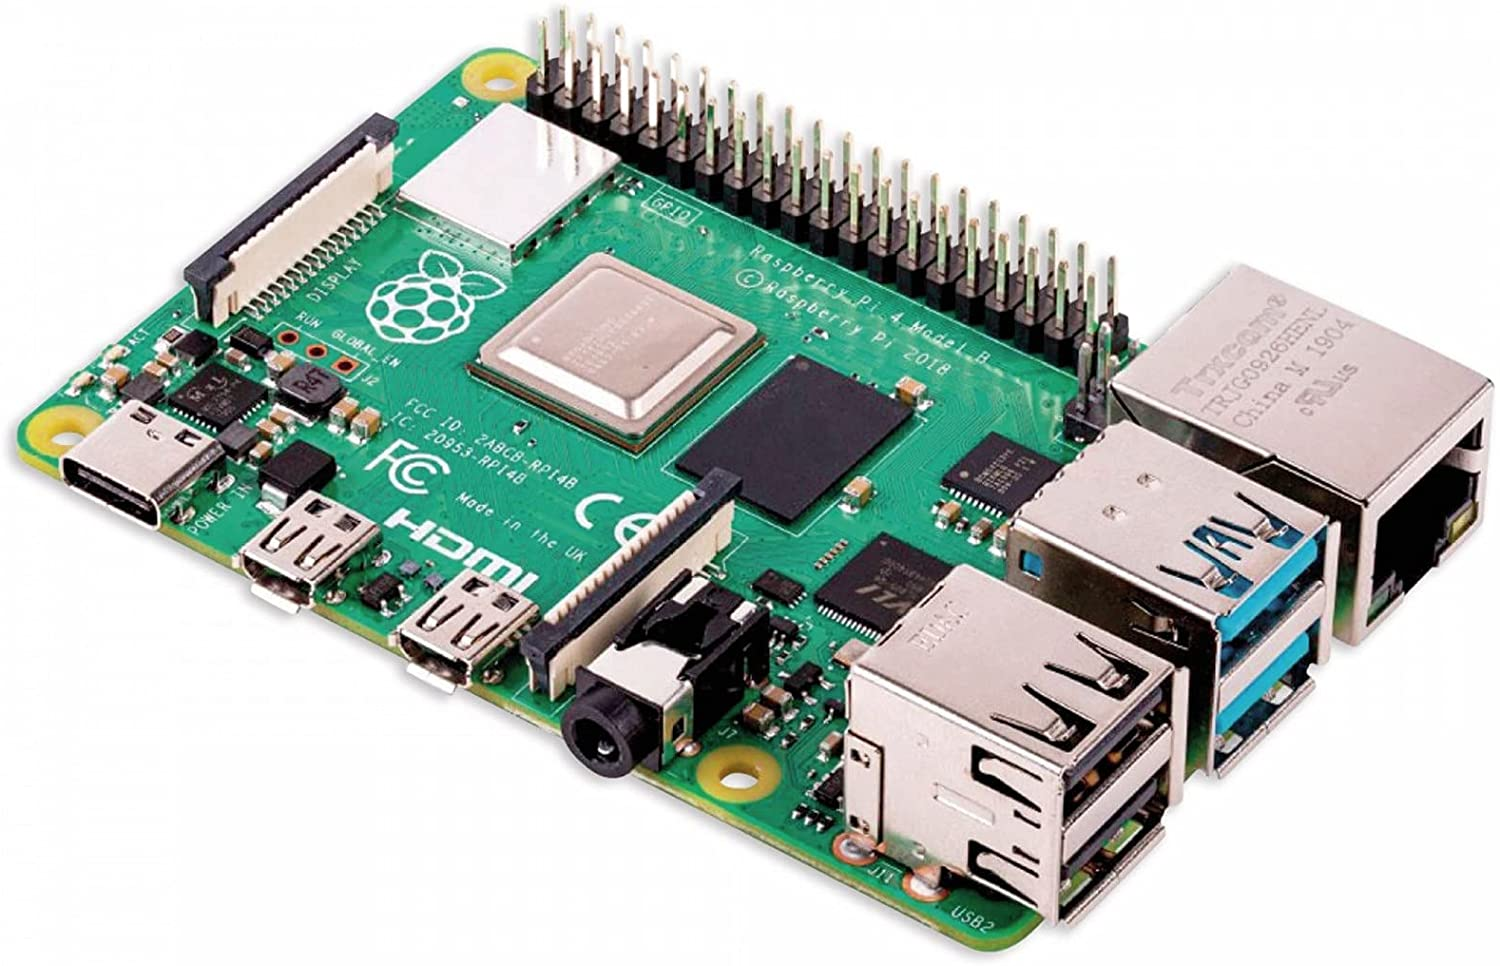
\includegraphics[width=8cm]{figs/raspberry.jpg}
  \end{center}
  \caption{Raspberry Pi 4b.}
  \label{fig:raspberry2}
\end{figure}

Sus características más atractivas ---entre otras--- son su bajo consumo energético, su pequeño tamaño y por lo tanto mínimo peso, su alta conectividad y puertos (red WIFI, Bluetooth, Ethernet, USB2 y USB3, HDMI, etc.) y la gran fluidez que posee su sistema operativo (Sección \ref{sec:raspberry_pi_os}). Todo esto la convierte en una potente y versátil placa, y son cada vez más los usuarios que la utilizan para diversos proyectos. Podemos encontrarla ---por ejemplo--- como centro doméstico inteligente para controlar la domótica de una casa, o incluso en sectores más profesionales formando parte de la arquitectura de algunos robots. Esto último es lo más interesante para nosotros, dentro de los múltiples usos que tiene una placa Raspberry.\\

\begin{table}[H]
\begin{center}
\begin{tabular}{|>{\arraybackslash}m{3cm} | >{\arraybackslash}m{6cm} |}
     \hline
     Procesador & Broadcom BCM2711 (4 núcleos Cortex-A72 (ARM v8), 64-bit, 1.5Ghz) \\ \hline
     Tarjeta gráfica & Broadcom VideoCore VI (integrada en el procesador) \\ \hline
     Memoria RAM & 4 GB LPDDR4-3200 SDRAM \\ \hline
     \multirow{3}{*}{Conexión}& WIFI 2.4 GHz y 5 GHz\\
     & Bluetooth 5.0/BLE\\
     & Gigabit Ethernet \\ \hline
     \multirow{5}{*}{Puertos}& 2 x micro-HDMI (4K 60 Hz)\\
     & MIPI Display Serial Interface \\
     & MIPI Camera Serial Interface \\
     & Jack Audio/Vídeo \\
     & Slot para micro-SD \\ \hline
     \multirow{2}{*}{Alimentación} & 5V por USB-C (3A mínimo) \\
     & 5V por GPIO (3A mínimo) \\ 
     \hline
 \end{tabular}
\caption{Especificaciones técnicas de la Raspberry Pi 4 Model B.}
\label{cuadro:especificaciones_rpi4}
\end{center}
\end{table}

Muchos de los robots son de tamaño reducido y no tienen el espacio suficiente como para acoplar una gran estación de procesamiento, por lo tanto en esos casos es muy común usar algún modelo de Raspberry como unidad central. Incluso en robots grandes se suelen utilizar también para realizar el control de zonas concretas, por ejemplo de los ojos de un humanoide. Por lo tanto, nuestro sistema de detección de emociones corriendo en la Raspberry Pi 4 Model B puede servir de gran ayuda a la hora de construir uno de estos robots comentados anteriormente que sólo tienen la capacidad de albergar una placa de tamaño reducido, o que simplemente los desarrolladores de dicho robot quieren ahorrar dinero en costes.

\subsection{Raspberry Pi OS}
\label{sec:raspberry_pi_os}

Raspberry Pi OS (Figura \ref{fig:captura_rpios}) es el sistema operativo oficial para Raspberry. Es un sistema operativo gratuito basado en Debian optimizado específicamente para el hardware de la Raspberry Pi, por lo tanto es el que mayor rendimiento nos ofrecerá frente a otros como Ubuntu (que también puede ser instalado). Además, está en constante desarrollo y continuamente se está mejorando su estabilidad y funcionalidad. Por todo ello, este será el sistema operativo elegido en nuestro proyecto, sobre todo por su alto rendimiento, algo esencial para impulsar el desempeño de nuestro sistema de detección de emociones.\\

\begin{figure} [h!]
  \begin{center}
    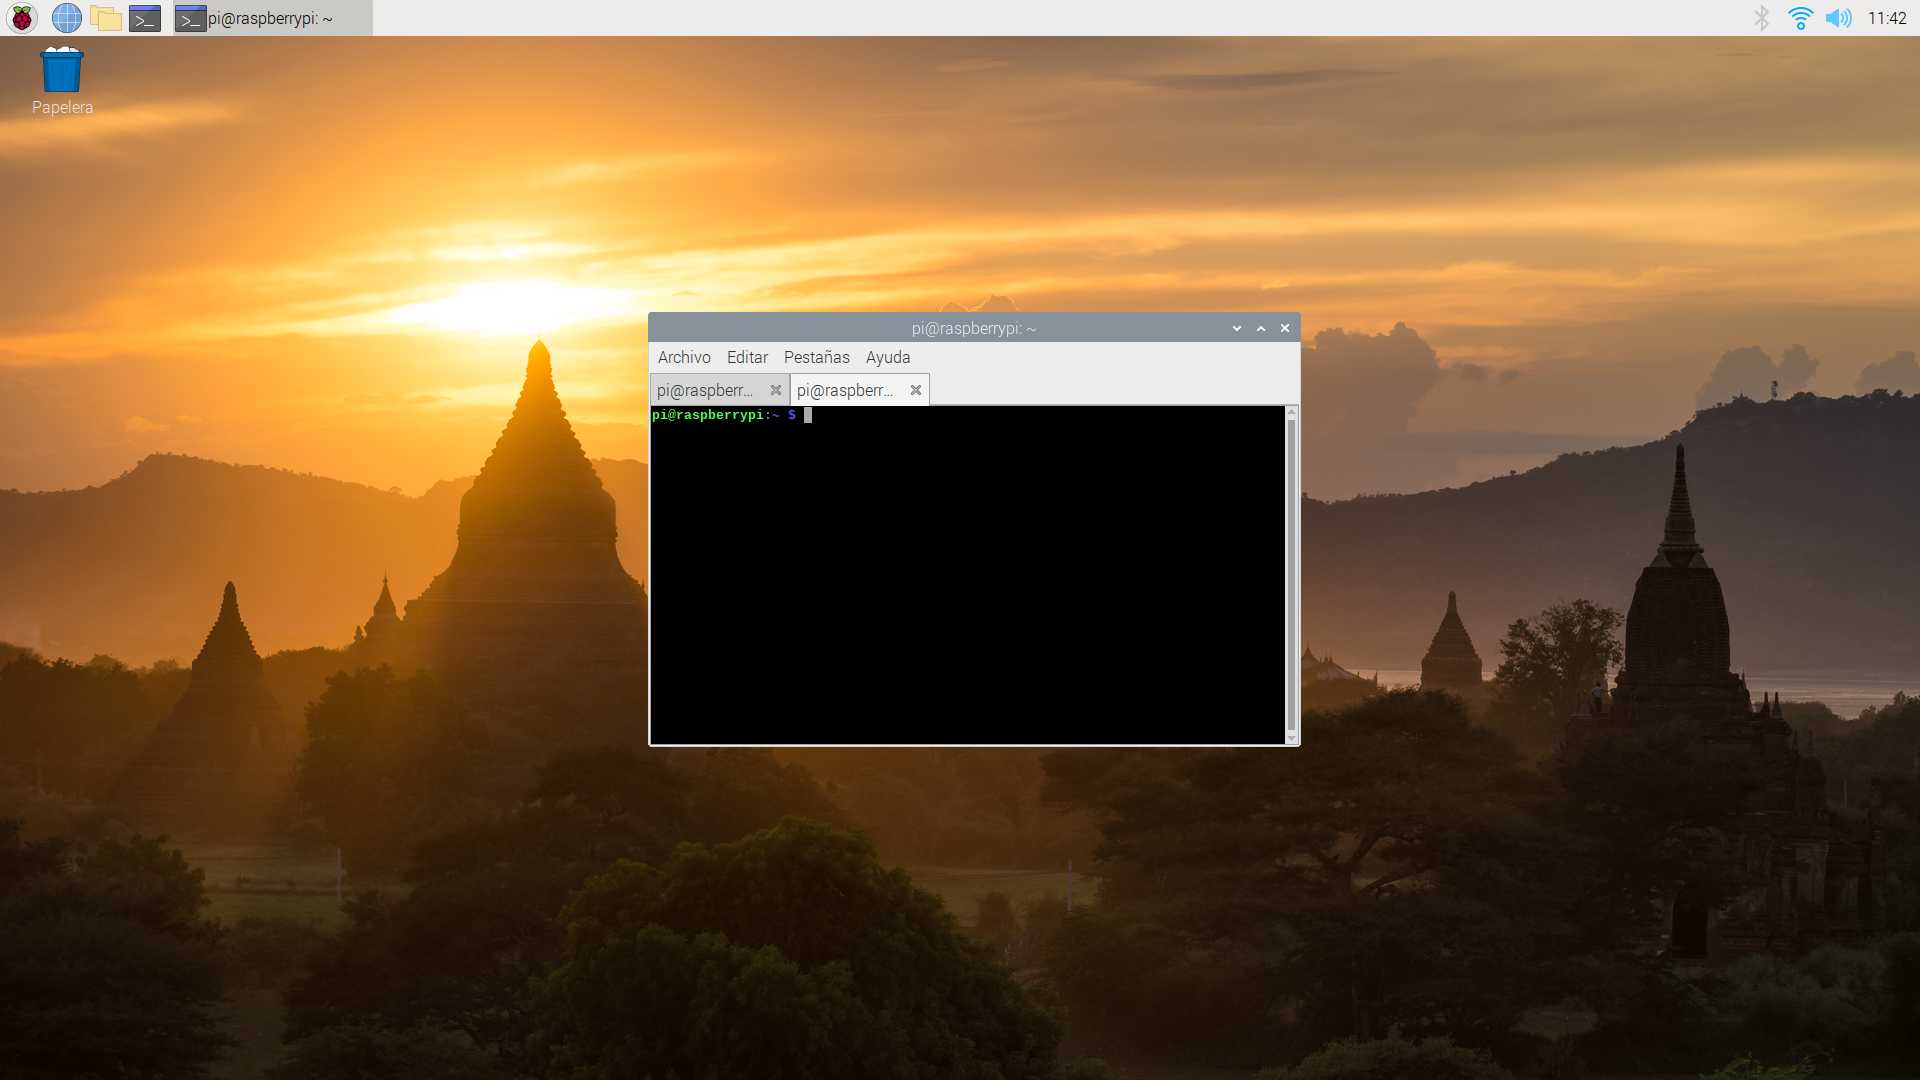
\includegraphics[width=14cm]{figs/captura_rpios.png}
  \end{center}
  \caption{Captura de pantalla de Raspberry Pi OS.}
  \label{fig:captura_rpios}
\end{figure}

La versión de Raspberry Pi OS escogida ha sido Raspberry Pi OS Legacy (Cuadro \ref{cuadro:especificaciones_rpios}). Se ha elegido dicha versión porque, de todas las disponibles, ha sido la única en la que se ha conseguido instalar una versión de ROS/ROS2 (en concreto, ROS Noetic). Además, aunque las versiones de Raspberry Pi OS de 64-bit ofrecían más rendimiento, todavía no estaban maduras y no ofrecían total compatibilidad con todas las librerías usadas en el presente trabajo.\\

\begin{table}[H]
\begin{center}
\begin{tabular}{|>{\arraybackslash}m{4cm} | >{\arraybackslash}m{4cm} |}
     \hline
     Fecha de lanzamiento & 4 de Abril de 2022 \\ \hline
     Sistema & 32-bit \\ \hline
     Versión del Kernel & 5.10 \\ \hline
     Versión de Debian & 10 (buster) \\ \hline
 \end{tabular}
\caption{Especificaciones de Raspberry Pi OS Legacy.}
\label{cuadro:especificaciones_rpios}
\end{center}
\end{table}

\subsection{Raspberry Pi Camera Module V2.1}
\label{sec:rpi_camera}

La Raspberry Pi Camera (Figura \ref{fig:rpi_camera}) es la cámara oficial desarrollada por Raspberry para ser utilizada en sus placas. Para este trabajo, se ha hecho uso de la versión 2.1 (Cuadro \ref{cuadro:especificaciones_rpi_camera}). Es una cámara de alta definición (3280x2464) que se conecta a cualquier Raspberry Pi compatible a través de una interfaz de bus CSI-2. Además de vídeo de alta calidad, ofrece una reducción de la contaminación de la imagen (ruido o manchas).\\

\begin{figure} [h!]
  \begin{center}
    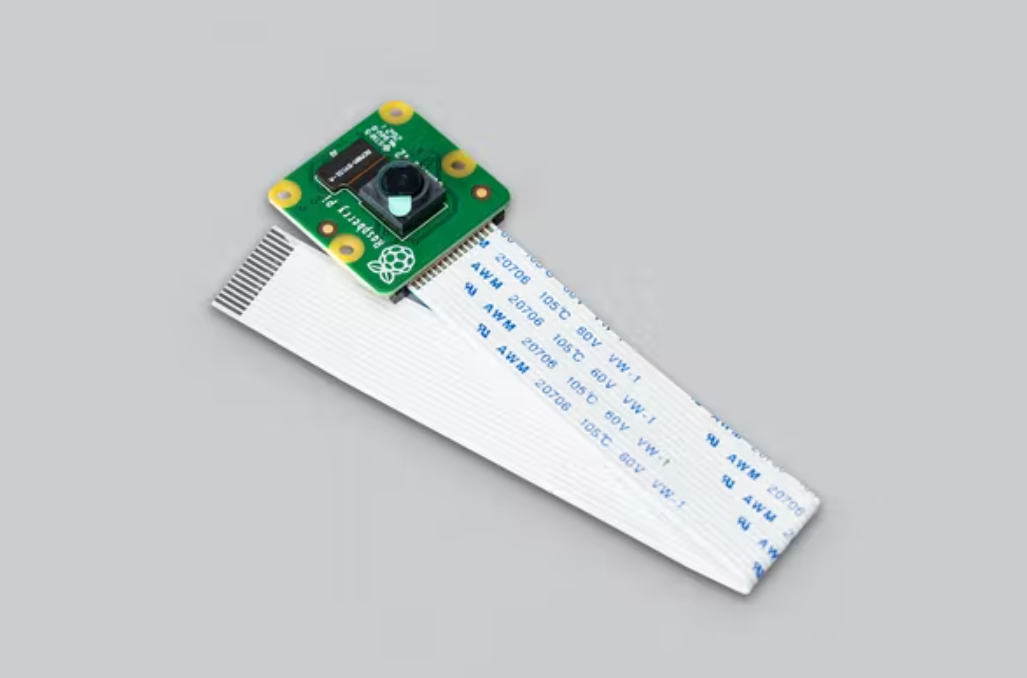
\includegraphics[width=9cm]{figs/rpi_camera.png}
  \end{center}
  \caption{Raspberry Pi Camera Module V2.1.}
  \label{fig:rpi_camera}
\end{figure}

\begin{table}[H]
\begin{center}
\begin{tabular}{|>{\arraybackslash}m{4cm} | >{\arraybackslash}m{6cm} |}
     \hline
     Sensor de imagen & Sony IMX 219 PQ CMOS \\ \hline
     Resolución de imagen & 3280x2464 (8-megapixeles) \\ \hline
     \multirow{2}{*}{Resolución de vídeo}& 1080p 30fps\\
     & 720p 60fps \\ \hline
     Conexión & Cable plano de 15 pines, MIPI Camera Serial Interfaze (CSI-2)\\ \hline
     Peso & 3g \\ \hline
     Dimensiones & 23.86 x 25 x 9 mm \\ \hline 
 \end{tabular}
\caption{Especificaciones de Raspberry Pi Camera Module V2.1.}
\label{cuadro:especificaciones_rpi_camera}
\end{center}
\end{table}

Se ha decidido escoger la Raspberry Pi Camera Module V2.1 en vez de una versión convencional de WebCam (USB) debido a las siguientes ventajas:

\begin{itemize}
    \item \textit{Mayor framerate.} Gracias a que la Raspberry Pi 4 Model B tiene un puerto dedicado para conectar la Raspberry Pi Camera (Figura \ref{fig:rpi_camera_CSI}), es posible conseguir una gran velocidad de fotogramas. Esto es debido a que esa conexión especial permite que la codificación vaya dirigida directamente a la GPU y sólo haya un pequeño impacto en la CPU, dejándola libre para otros usos. En cambio, una WebCam conectada por USB utiliza directamente la CPU, y mover datos a través de un USB es bastante costoso para un sistema de recursos limitados.
    
    \begin{figure} [h!]
      \begin{center}
        \includegraphics[width=9cm]{figs/rpi_camera_CSI.JPG}
      \end{center}
      \caption{MIPI Camera Serial Interfaze (CSI-2).}
      \label{fig:rpi_camera_CSI}
    \end{figure}
    
    \item \textit{Mayor calidad de imagen.} Es cierto que también existen WebCam con una calidad de imagen muy buena, pero su precio es elevado. Por lo tanto, la Raspberry Pi Camera acaba ganando en cuanto a calidad de imagen si realizamos la comparativa en el mismo rango de precio (29,14 \euro\footnote{Distribuidor oficial de Raspberry: \url{https://www.kubii.es/318-camaras-sensores}}). Sin embargo, este no es un apartado muy relevante porque finalmente en el sistema de detección de emociones no hacemos uso de la máxima resolución para aumentar el rendimiento.
    
    \item \textit{Menor tamaño.} El tamaño tan compacto de la Raspberry Pi Camera es uno de sus mayores atractivos y es por eso que es también una gran ventaja frente a las WebCam. De cara a instalar estos pequeños ordenadores con cámara en un robot es esencial que ocupen el menor espacio posible, además de que su peso sea muy reducido.
\end{itemize}

\section{Python}

Python es un lenguaje de programación interpretado (se ejecuta sin necesidad de ser compilado) y de tipado dinámico (las variables se comprueban en tiempo de ejecución). Es de licencia totalmente libre y soporta programación orientada a objetos. Se caracteriza por hacer uso de una sintaxis muy legible en la que es obligatoria una correcta tabulación.\\

Se ha escogido Python (versión 3.7.3) como lenguaje de programación para este proyecto debido a los dos siguientes motivos:

\begin{enumerate}
    \item El sistema desarrollado en este trabajo usa algoritmos de Machine Learning para detectar las emociones faciales, y Python es el lenguaje de programación rey en ese campo; posee múltiples librerías como Pandas, TensorFlow, Keras, Scikit-learn... que brindan un soporte excepcional para cualquier tarea relacionada con el aprendizaje automático.
    
    \item La librería que da soporte oficial a la Raspberry Pi Camera (Sección \ref{sec:rpi_camera}) únicamente se puede usar en Python. Se trata del paquete \textit{picamera}.
\end{enumerate}

A continuación se enumerarán los módulos de Python usados en el desarrollo del presente trabajo:

\begin{itemize}
    \item \textit{NumPy} (1.21.6). Ofrece una gran colección de funciones matemáticas de alto nivel y permite crear y trabajar con vectores y matrices multidimensionales.
    
    \item \textit{OpenCV} (4.5.5.64). Es la biblioteca más popular de Visión Artificial, ofrece múltiples herramientas de procesamiento de imágenes.
    
    \item \textit{pandas} (1.3). Usada para manipulación y análisis de datos.
    
    \item \textit{threading} (1.4.6). Proporciona soporte para poder utilizar hilos.
    
    \item \textit{pickle} (5.3.4). Permite serializar y deserializar objetos de Python.
    
    \item \textit{math} (7.1.3). Ofrece funciones matemáticas de alto nivel.
    
    \item \textit{argparse} (2.5.4). Permite crear interfaces de línea de comandos de forma sencilla.
    
    \item \textit{matplotlib} (4.7.1). Librería muy completa para la generación de gráficas estáticas e interactivas.
    
    \item \textit{glob} (9.3.4). Permite navegar por los archivos y directorios del sistema utilizando expresiones regulares.
    
    \item \textit{picamera} (3.2.4). Ofrece soporte para la Raspberry Pi Camera en Python.
    
    \item \textit{MediaPipe} (3.2.1). Explicado en profundidad en la Sección \ref{sec:mediapipe}.
    
    \item \textit{dlib} (5.7.1). Explicado en profundidad en la Sección \ref{sec:dlib}.
    
    \item \textit{Scikit-learn} (2.6.3). Explicado en profundidad en la Sección \ref{sec:sklearn}.
\end{itemize}

\section{MediaPipe}
\label{sec:mediapipe}

MediaPipe\footnote{MediaPipe: \url{https://mediapipe.dev/}} es una plataforma, perteneciente a Google, que ofrece soluciones \textit{open source} (código libre) de Machine Learning para varias plataformas: Android, iOS, C++, Python, Javascript y Coral. Se caracteriza por ofrecer algoritmos muy rápidos capaces de funcionar con valores altos de FPS sin hacer uso de una GPU. Se puede encontrar el código de todas las herramientas que ofrece en su repositorio de GitHub\footnote{Repositorio MediaPipe: \url{https://github.com/google/mediapipe}}.

\subsection{Face Mesh}

MediaPipe Face Mesh\footnote{MediaPipe Face Mesh: \url{https://google.github.io/mediapipe/solutions/face_mesh}} es una de las soluciones que nos ofrece MediaPipe. Se trata de una herramienta que detecta una malla facial 3D compuesta por 468 puntos usando únicamente una cámara (Figura \ref{fig:mediapipe}). Haremos uso de este sistema en este trabajo para obtener información, en forma de coordenadas, de puntos faciales característicos.\\

\begin{figure} [h!]
  \begin{center}
    
\includegraphics[width=12cm]{figs/mediapipe.png}
  \end{center}
  \caption{Malla facial de MediaPipe.}
  \label{fig:mediapipe}
\end{figure}

La arquitectura de Face Mesh está compuesta por dos modelos de Machine Learning (redes neuronales profundas): un detector facial y otro que predice la superficie 3D de puntos faciales usando únicamente el sector de las caras detectadas, este último desarrollado en el artículo \cite{facemesh_surface}. Tener la cara recortada previamente aumenta el rendimiento. Además, una vez que se han detectado los rostros y se han localizado los puntos de referencia faciales, en los siguientes fotogramas simplemente se procede a realizar un rastreo de dichos puntos en vez de realizar constantemente detecciones (faciales o de coordenadas). Una vez que se pierdan, ya sí que se lleva a cabo una nueva detección.\\

La herramienta posee los siguientes parámetros de entrada que permiten personalizar su funcionamiento:
\begin{itemize}
    \item \verb|static_image_mode|: se indica con un booleano (\textit{True} o \textit{False}) si se va a procesar una imagen estática o un vídeo, para que en caso de que sea un vídeo, realizar las optimizaciones oportunas.
    
    \item \verb|max_num_faces|: se indica con un número entero el número de caras que se desean detectar como máximo.
    
    \item \verb|refine_landmarks|: aumenta la precisión de las coordenadas alrededor de los ojos y los labios, a cambio de un poco más de cómputo. Se activa o desactiva con un booleano (\textit{True} o \textit{False}).
    
    \item \verb|min_detection_confidence|: con un valor del intervalo [0.0, 1.0] se indica al modelo de detección de rostros el valor mínimo de confianza para considerar una predicción exitosa.
    
    \item \verb|min_tracking_confidence|: con un valor del intervalo [0.0, 1.0] se indica al modelo de puntos faciales el valor mínimo de confianza para considerar que los puntos han sido rastreados correctamente.
\end{itemize}

La salida que nos proporciona exactamente el sistema Face Mesh de Mediapipe es una colección de rostros, donde cada rostro se representa como una lista de 468 puntos y cada uno de esos puntos se compone de las variables \textit{x}, \textit{y} y \textit{z}. Las variables \textit{x} e \textit{y} están normalizadas entre 0 y 1, por el ancho y alto de la imagen. La variable \textit{z} contiene la profundidad del punto, siendo el origen el centro de la cabeza.

\section{Detector de puntos faciales de dlib.}
\label{sec:dlib}

Dlib es un conjunto de herramientas que contiene algoritmos de Machine Learning. En este trabajo se ha hecho uso del detector de puntos faciales, capaz de detectar 68 puntos de referencia, contenido en dlib (Figura \ref{fig:dlib_example}).\\

\begin{figure} [h!]
  \begin{center}
    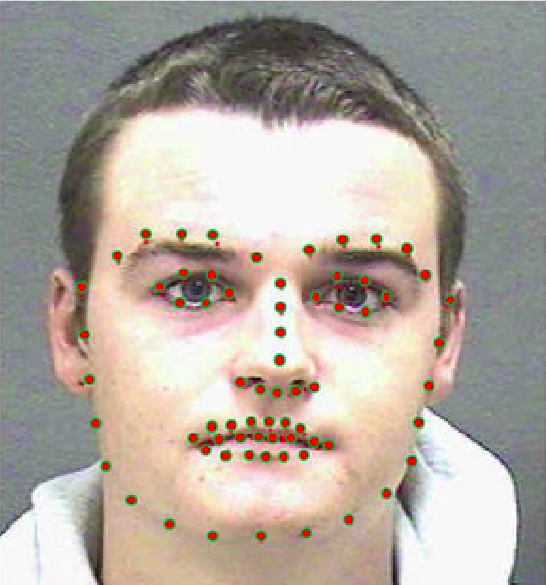
\includegraphics[width=70mm]{figs/dlib_example.png}
  \end{center}
  \captionsetup{justification=centering}
  \caption{Ejemplo usando el detector de puntos faciales de dlib.\\
  Imagen obtenida del artículo \cite{dlib_example}}
  \label{fig:dlib_example}
\end{figure}

El algorimo está compuesto de dos fases: detección del rostro y detección de las regiones faciales. Para realizar la detección de rostros, dlib incluye dos opciones:

\begin{itemize}
    \item HOG (Histogram of Oriented Gradients) y Linear SVM.
    \item Red Neuronal Convolucional MMOD (Max-Margin Object Detection)
\end{itemize}

Posteriormente, para realizar la detección de puntos de referencia faciales, usa Árboles de Regresión. En concreto, usa la técnica explicada en el artículo \cite{facial_landmarks_dlib}

\section{Scikit-learn. Algoritmos de Machine Learning}
\label{sec:sklearn}

Scikit-learn\footnote{Scikit-learn: \url{https://scikit-learn.org/stable/}} es una librería open source para Python que ofrece herramientas de Machine Learning. Entre ellas, incluye varios algoritmos de clasificación, los cuales serán usados en este trabajo. En las siguientes secciones se explica el funcionamiento de cada uno de ellos.

\subsection{Máquinas de Vector Soporte (SVM)}

Las \textit{Máquinas de Vector Soporte} o SVM (Support Vector Machines) son algoritmos de aprendizaje supervisado que se utilizan para resolver tareas de clasificación. El concepto general en el que está basado SVM es el de la generación de un hiperplano que separa los datos de una clase con respecto a otra. La separación se realizará con la máxima distancia entre los puntos y el hiperplano; esto es, se separarán los datos de la forma más óptima posible (Figura \ref{fig:svm_hiperplano}). El dato más cercano al hiperplano de cada clase se denomina vector soporte.\\

\begin{figure} [h!]
  \begin{center}
    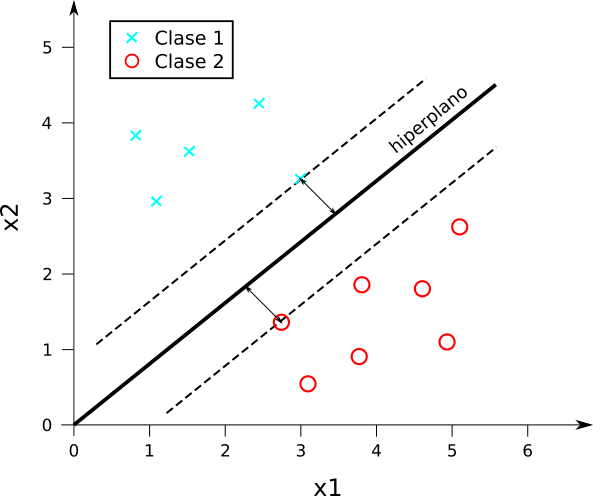
\includegraphics[width=95mm]{figs/svm_hiperplano.png}
  \end{center}
  \caption{Hiperplano de separación óptimo entre\\
            los datos de dos clases.}
  \label{fig:svm_hiperplano}
\end{figure}

El ejemplo de la Figura \ref{fig:svm_hiperplano} es separable linealmente (usando como hiperplano una línea), pero en la práctica real es complicado que esto suceda. Por eso, normalmente se hace uso de lo que se denomina \textit{kernel}, para transformar el conjunto de datos a un nuevo conjunto de una dimensión mayor y que, de esta manera, se puedan separar linealmente en su nueva dimensión.

\subsection{K Vecinos más Cercanos (KNN)}

El \textit{K Vecinos más Cercanos} o KNN (K-Nearest Neighbours) es un algoritmo de aprendizaje supervisado utilizado para resolver tareas de clasificación. A diferencia de otros métodos, este utiliza siempre el conjunto de entrenamiento completo para realizar predicciones, en vez de crear un modelo en base a la relación de las entradas y las salidas. Es por ello que es un método costoso computacionalmente para conjuntos de datos muy grades, pero ese no es nuestro caso.\\

El método está basado en calcular la distancia del dato a evaluar respecto a los demás datos. Partiendo de eso, el algoritmo se queda con los \textit{k} datos más cercanos, siendo \textit{k} un parámetro personalizable, y de estos elige la clase que más se repite, siendo esta la predicción realizada (Figura \ref{fig:knn}). Para medir la distancia entre datos, el método utilizado en este trabajo es el de distancia Euclídea (Ecuación \ref{ec:d_euclidea}).\\

\begin{figure} [h!]
  \begin{center}
    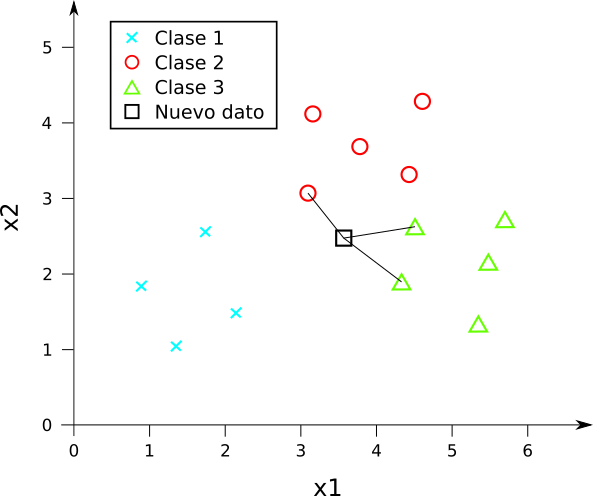
\includegraphics[width=95mm]{figs/knn.png}
  \end{center}
  \captionsetup{justification=centering}
  \caption{Ejemplo de KNN con $k = 3$.}
  \label{fig:knn}
\end{figure}

\begin{myequation}[h]
\begin{equation}
d(x^{\prime}, x^{(i)}) = \sqrt{\sum_{r=1}^{p}(x_{r}^{\prime}-x_{r}^{(i)})^{2}}
\nonumber
\label{ec:d_euclidea}
\end{equation}
\captionsetup{justification=centering}
\caption[Distancia Euclídea de un vector $x^{\prime}$ con \textit{p} características respecto al vector i-ésimo $(x^{(i)})$]{Distancia Euclídea de un vector $x^{\prime}$ \\
con \textit{p} características respecto al vector i-ésimo $(x^{(i)})$}
\end{myequation} 

\subsection{Redes Neuronales Multicapa}

Una red neuronal (Figura \ref{fig:red_neuronal}) es un modelo computacional inspirado en el funcionamiento del cerebro humano, y es utilizado en la mayoría de los casos como técnica de aprendizaje supervisado. Está compuesta por un conjunto de neuronas que, a su vez, si la red es multicapa, forman capas de neuronas. Existen también redes neuronales de una sola capa, denominadas perceptrón.\\

\begin{figure} [h!]
  \begin{center}
    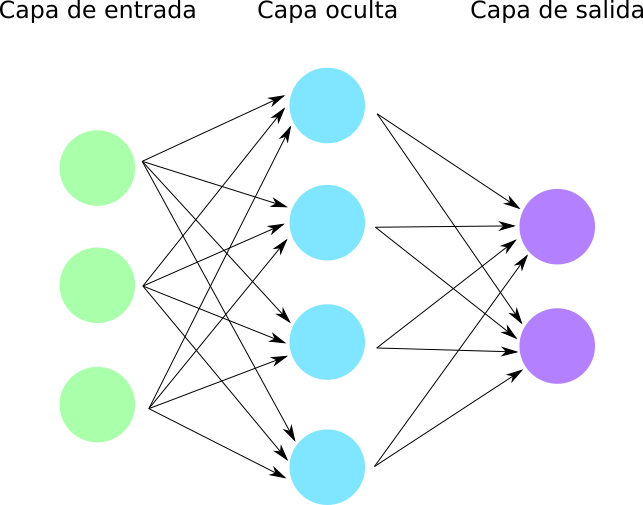
\includegraphics[width=11cm]{figs/redes_neuronales.png}
  \end{center}
  \caption{Red neuronal de tres capas y ocho neuronas.}
  \label{fig:red_neuronal}
\end{figure}

Todas las neuronas están interconectadas entre sí y cada una de esas neuronas estará formada por una función de decisión o función de transferencia (normalmente una función escalón, lineal o sigmoide). En el caso de una neurona de una sola entrada, la función de decisión evaluará la suma del producto del peso \textit{w} y la entrada \textit{x}, más el término independiente \textit{b} (Figura \ref{fig:neurona}).\\

\begin{figure} [h!]
  \begin{center}
    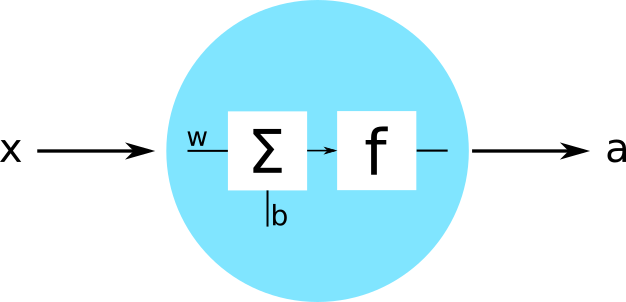
\includegraphics[width=8cm]{figs/neurona.png}
  \end{center}
  \captionsetup{justification=centering}
  \caption{Ejemplo del interior de una neurona de una entrada,\\
  donde \textit{x} es la entrada y \textit{a} es la salida.}
  \label{fig:neurona}
\end{figure}

La etapa de \textit{entrenamiento} será un proceso iterativo en el que la red neuronal ajustará los valores de los pesos \textit{w} de cara a estimar el valor de salida.  Una vez que se haya finalizado el entrenamiento, la red se usa como una \textit{caja negra}; esto es, se le proporcionan una serie de entradas, y esta devuelve sus respectivas salidas, sin nosotros conocer lo que ha sucedido dentro.

\subsection{Análisis de Componentes Principales (PCA)}

El Análisis de Componentes Principales o PCA (Principal Component Analysis) es un método de reducción de dimensionalidad que permite reducir el número de características de entrada que componen el conjunto de datos, a la vez que se conserva la información. Esto se consigue utilizando relaciones entre características que se pueden detectar mediante el cálculo de autovectores y autovalores de la matriz de covarianza que se genera a partir de los datos de entrada.\\

\noindent
Entre las ventajas que nos proporciona este método, encontramos:

\begin{itemize}
    \item Crear un dataset más eficiente y, por lo tanto, reducir el sobreajuste y aumentar la precisión a la hora de realizar un entrenamiento con los datos.
    
    \item Reducir la carga computacional de los algoritmos de aprendizaje.
\end{itemize}

\section{ROS (Robot Operating System)}

ROS (Robot Operating System)\footnote{ROS: \url{https://www.ros.org/}} (Figura \ref{fig:logo_ros}) es un \textit{middleware} para el desarrollo de software en robots, es decir, una colección de librerías software que proporcionan servicios tales como la abstracción del hardware o paso de mensajes entre procesos. Además, todo es código libre y multiplataforma (Linux, Windows, macOS).\\

\begin{figure} [h!]
  \begin{center}
    \includegraphics[width=5cm]{figs/ros_logo.png}
  \end{center}
  \captionsetup{justification=centering}
  \caption{Logo de ROS.}
  \label{fig:logo_ros}
\end{figure}

Cada uno de los procesos de ROS se denominan \textit{nodos}, y se comunican entre sí usando \textit{topics}, ya sea en la misma máquina o de forma remota en una red local. El envío y recibimiento de mensajes a través de los \textit{topics} se consigue haciendo uso de publicadores y subscriptores. Además, ofrece otras opciones de comunicación como los servicios o acciones. El nodo \textit{máster} será el encargado de permitir que todos los nodos se localicen entre sí, proporcionando ---entre otras cosas--- servicios de \textit{naming}. En la Figura \ref{fig:ros} se puede observar un esquema reducido de lo que sería una comunicación entre un nodo publicador y un nodo suscriptor a través del \textit{topic} \verb|/ejemplo|.\\

\begin{figure} [h!]
  \begin{center}
    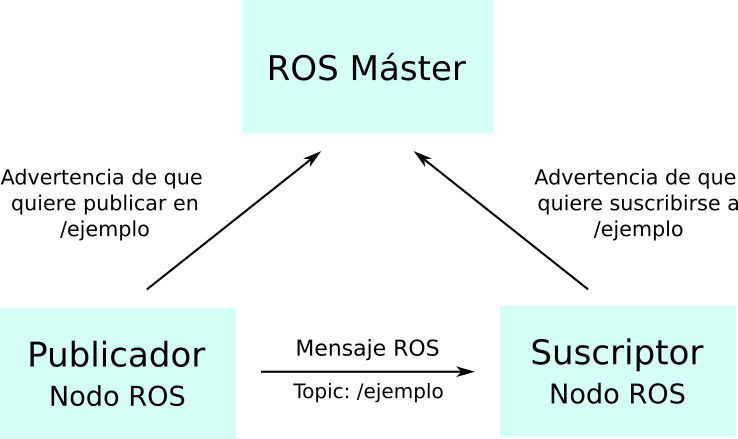
\includegraphics[width=11cm]{figs/ros.png}
  \end{center}
  \captionsetup{justification=centering}
  \caption{Esquema simple de una comunicación publicador-suscriptor en ROS.}
  \label{fig:ros}
\end{figure}

Existe una gran comunidad de usuarios desarrolladores que aportan paquetes al entorno ROS y, por lo tanto, lo hacen aún más rico. Entre todos estos paquetes, podemos encontrar algunos enfocados en ---por ejemplo--- identificación de objetos o reconocimiento de voz. La versión de ROS usada en este trabajo será ROS Noetic y el resultado final del sistema será de código libre para dicha comunidad de ROS.

\chapter{Desarrollo del sistema}
\label{cap:capitulo4}

En este capítulo se describe todo el proceso llevado a cabo durante el desarrollo del sistema de detección de emociones y su posterior integración en ROS. Además, se muestran ejemplos de su funcionamiento y se realizan pruebas de rendimiento.

\section{Método de detección de emociones}

Existen múltiples técnicas utilizadas para realizar detección de emociones, en el artículo \cite{literature_review} encontramos una revisión del estado del arte de los últimos años. En este trabajo, se ha escogido la técnica comprendida por los siguientes tres pasos: detección de puntos faciales, extracción de información de esos puntos faciales, clasificación de esa información (Figura \ref{fig:metodo}).\\

\begin{figure} [h!]
  \begin{center}
    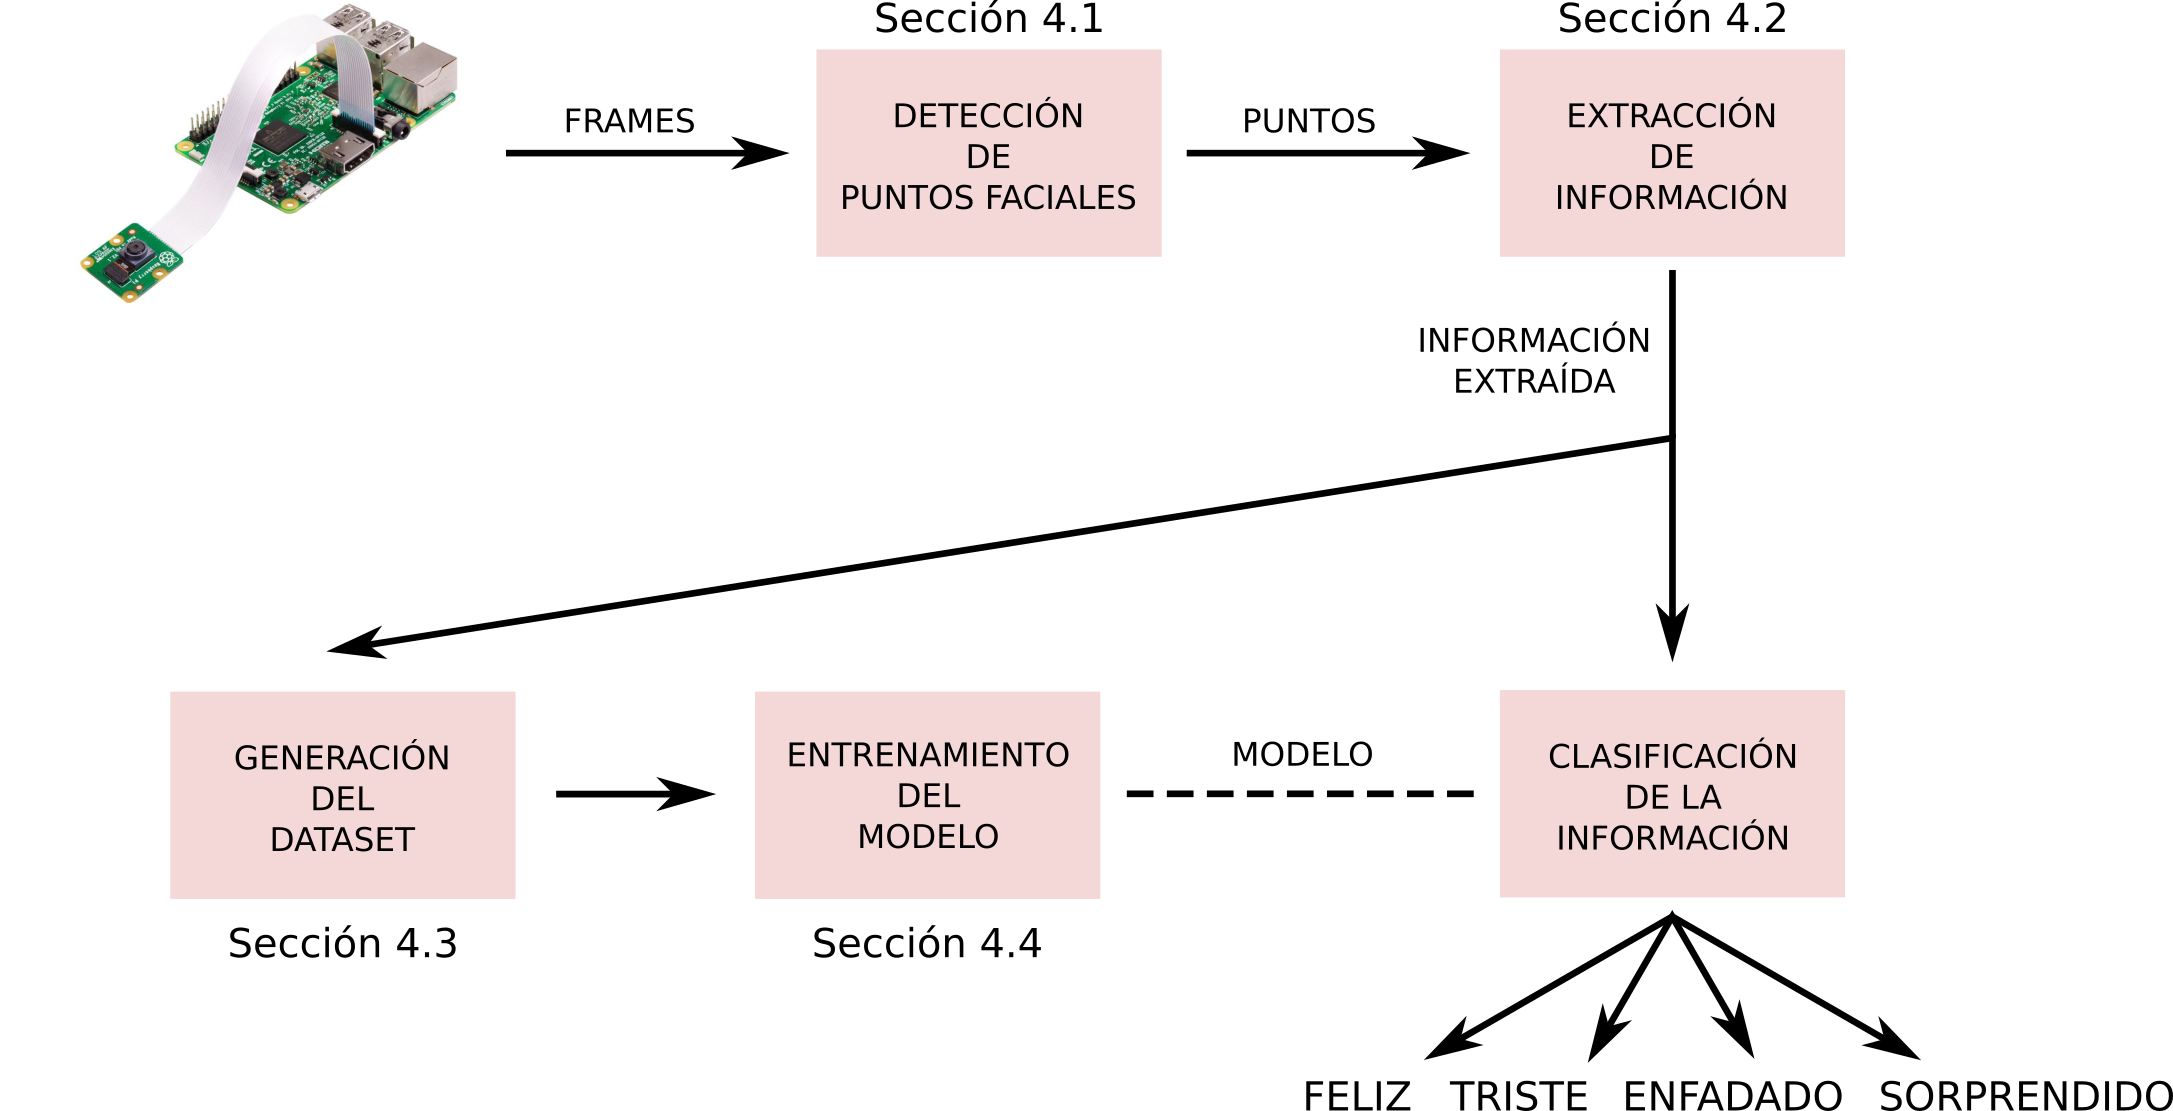
\includegraphics[width=16cm]{figs/metodo.png}
  \end{center}
  \captionsetup{justification=centering}
  \caption{Método de detección de emociones.}
  \label{fig:metodo}
\end{figure}

El motivo de esta elección es debido a que es un método con bajo coste computacional y además es de los más precisos, algo esencial para aportar robustez a la herramienta robótica final de este trabajo.

\section{Detección de puntos faciales}

El primer paso del método escogido en este trabajo, consiste en realizar una detección de puntos faciales característicos. En búsqueda de la máxima optimización, se va a hacer un estudio comparando dos librerías de extracción de puntos faciales para obtener conclusiones de cual de ellas nos ofrece más rendimiento y precisión. Las dos librerías son dlib (Sección \ref{sec:dlib}) y MediaPipe (Sección \ref{sec:mediapipe}), escogidas por ser las más usadas dentro de la investigación de este campo en publicaciones como, por ejemplo, los artículos \cite{dlib_emotions} o \cite{mediapipe_emotions}.\\

Las pruebas se realizarán en la Raspberry Pi 4 Model B bajo Raspberry Pi OS, usando la Raspberry Pi Camera como dispositivo para capturar vídeo. Se puede encontrar más información sobre las versiones usadas en el Capítulo \ref{cap:capitulo3}. La resolución utilizada será de 640x480 píxeles y se parte de una media en crudo de 20fps, esto es, sólo mostrando los \textit{frames} (capturados con la librería \textit{picamera}) por pantalla sin ningún tipo de procesamiento.

\subsection{Dlib}

Se comenzará estudiando el rendimiento en FPS ofrecido por dlib y posteriormente se hará un estudio de los fallos producidos por el algoritmo en distintas situaciones. Para realizar las pruebas de rendimiento, se guardará el valor de fps calculado para cada \textit{frame} durante 30 segundos y posteriormente se calculará la media de dichos \textit{frames} guardados. Para realizar las pruebas de fallos, se tendrán en cuenta dos situaciones: falsos positivos y no detección de ningún rostro. Se dará por hecho que siempre hay una cara en cada \textit{frame}, por lo tanto, un \textit{falso positivo} significa que hay más de una cara y \textit{no detección} significa que no hay ninguna. Entonces, se evaluará cada \textit{frame} durante 30 segundos siguiendo esos criterios, y se hará un recuento de los fallos.

\subsubsection{Prueba 1 de rendimiento}

Tal como se ha explicado en la Sección \ref{sec:dlib}, dlib divide la extracción de características faciales en dos pasos: detección del rostro y extracción de características. Para el primero de los pasos, se ofrecen dos opciones incorporadas en sus librerías (HOG y Linear SVM o CNN). En la primera prueba haremos uso del detector de caras basado en HOG y Linear SVM, ya que es el más eficiente computacionalmente hablando, sumado al detector de características también incorporado en las librerías de dlib. Esto ofrece un rendimiento de 0.83 fps de media.

\subsubsection{Prueba 2 de rendimiento}

Tras comprobar el bajo rendimiento obtenido en la primera prueba, se procederá a sustituir el detector de caras usado anteriormente por el detector de caras que trae incorporado OpenCV, este es descrito en el artículo \cite{opencv_haar_cascade}. Se hace uso de este algoritmo porque actualmente es uno de los más rápidos realizando detección facial. Este cambio impulsa el rendimiento de dlib un 656\%, obteniendo una media de 6.28 fps.

\subsubsection{Prueba 3 de rendimiento}
Con el objetivo de mejorar aún más el rendimiento, se procederá a dividir el procesamiento de los \textit{frames} de la lectura de los mismos, haciendo uso de threads. De esta manera se aprovecharán los 4 núcleos del procesador ARM de la Raspberry Pi 4 Model B. Para esto, lo que haremos es lanzar un \textit{thread} que se encargue constantemente de realizar la lectura de los \textit{frames} usando la librería \textit{picamera}, y por otro lado, el thread principal del programa se encargará de realizar el procesamiento de dlib y el detector de caras de OpenCV. Con esto impulsamos el rendimiento un 30\% más, logrando así una media de 8.21 fps. Se puede ver una comparativa de las tres pruebas de rendimiento en la Figura \ref{fig:dlib_rendimiento}.

\begin{figure} [h!]
  \begin{center}
    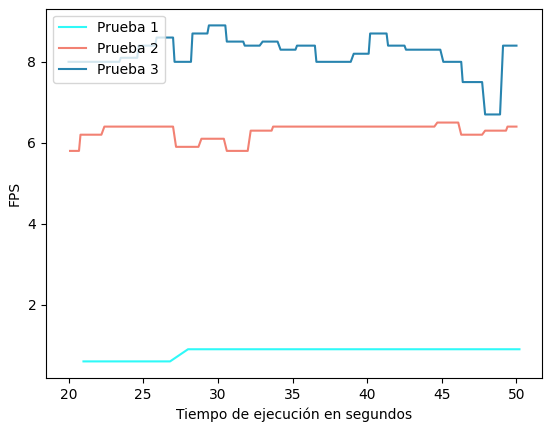
\includegraphics[width=10cm]{figs/dlib_rendimiento.png}
  \end{center}
  \captionsetup{justification=centering}
  \caption{Comparativa de las tres pruebas de rendimiento de dlib.}
  \label{fig:dlib_rendimiento}
\end{figure}

\subsubsection{Prueba de fallos}

Para comprobar la robustez del algoritmo, se evaluará a este en las siguientes condiciones (Figura \ref{fig:dlib_fallos_ejemplos}):

\begin{itemize}
    \item Buenas condiciones lumínicas: 81 fallos.
    \item Malas condiciones lumínicas: 126 fallos.
    \item Rostros parcialmente cubiertos: 188 fallos.
    \item Rostros girados: 183 fallos.
\end{itemize}

\begin{figure}[h!]
  \begin{center}
    \subcapcentertrue
    \subfigure[Buenas condiciones de luz]{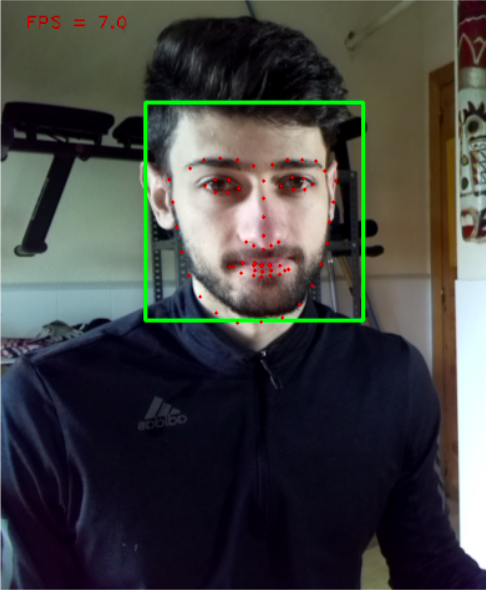
\includegraphics[width=37mm]{figs/dlib_buena_luz.png}}
    \subfigure[Malas condiciones de luz]{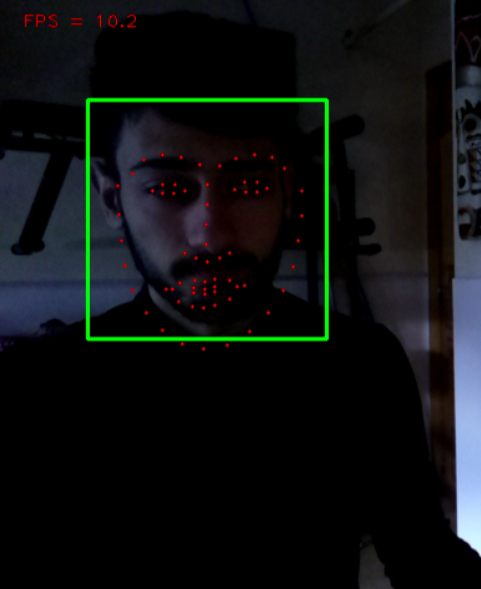
\includegraphics[width=37mm]{figs/dlib_mala_luz.png}}
    \subfigure[Rostros cubiertos]{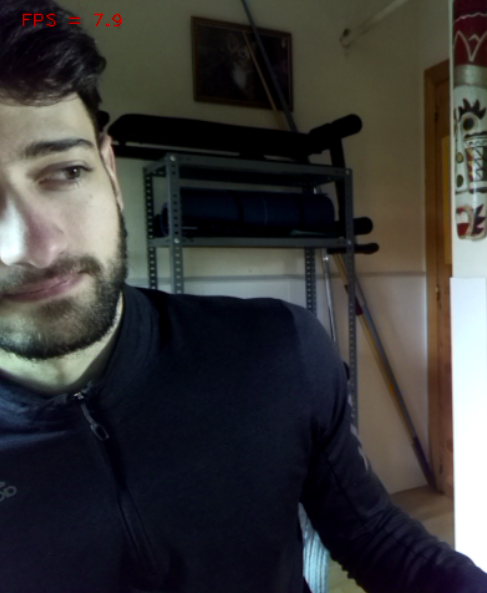
\includegraphics[width=37mm]{figs/dlib_cubiertos.png}}
    \subfigure[Rostros girados]{
\includegraphics[width=37mm]{figs/dlib_girados.png}}
  \end{center}
\caption{Condiciones en las que se evalúan los fallos de dlib.}
\label{fig:dlib_fallos_ejemplos}
\end{figure}

\subsection{MediaPipe}
Se comenzará estudiando el rendimiento en FPS ofrecido por MediaPipe y posteriormente se hará un estudio de los fallos producidos por el algoritmo en distintas situaciones. Para realizar las pruebas de rendimiento, se guardará el valor de fps calculado para cada \textit{frame} durante 30 segundos y posteriormente se calculará la media de dichos \textit{frames} guardados. Para realizar la prueba de fallos, a diferencia de dlib, sólo se evaluarán las no detecciones porque los falsos positivos se pueden evitar indicando al algoritmo que sólo detecte una cara. Entonces, se evaluará cada \textit{frame} durante 30 segundos siguiendo esos criterios, y se hará un recuento de los fallos.

\subsubsection{Prueba 1 de rendimiento}
En esta primera prueba se utilizará el algoritmo de la forma general recomendada en el tutorial oficial de MediaPipe. De esta manera, obtenemos una media de 5.91 fps. Este dato es inferior al resultado final de 8.21 fps de dlib.

\subsubsection{Prueba 2 de rendimiento}
Llegados a este punto, para mejorar el resultado anterior, dividimos el procesamiento total en \textit{threads} al igual que hicimos con dlib. Dedicamos un \textit{thread} a la lectura de \textit{frames} y el \textit{thread} principal al procesamiento de MediaPipe. De esta manera, aumentamos el rendimiento un 32\%, obteniendo una media de 7.80fps, todavía sin superar el mejor desempeño de dlib.

\subsubsection{Prueba 3 de rendimiento}
Hasta ahora, estábamos mostrando por pantalla la malla facial detectada, pero esto no será necesario cuando implementemos nuestro sistema de detección de emociones. Por ello, se analizará el rendimiento sin dibujar dicha malla en cada \textit{frame}. De esta manera, el rendimiento sube un 70\% más, llegando así ya a una media de 13.28 fps. Se puede ver una comparativa de las tres pruebas de rendimiento en la Figura \ref{fig:mediapipe_rendimiento}

\begin{figure} [h!]
  \begin{center}
    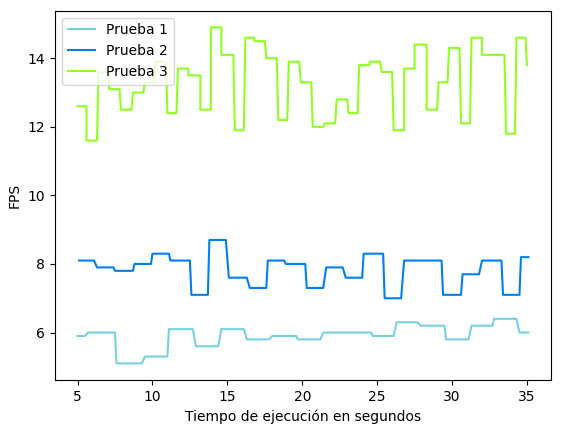
\includegraphics[width=10cm]{figs/mediapipe_rendimiento.png}
  \end{center}
  \captionsetup{justification=centering}
  \caption{Comparativa de las tres pruebas de rendimiento de MediaPipe.}
  \label{fig:mediapipe_rendimiento}
\end{figure}

\subsubsection{Prueba de fallos}

Para comprobar la robustez del algoritmo, se evaluará a este en las siguientes condiciones (Figura \ref{fig:mediapipe_fallos_ejemplos}):

\begin{itemize}
    \item Buenas condiciones lumínicas: 0 fallos.
    \item Malas condiciones lumínicas: 0 fallos.
    \item Rostros parcialmente cubiertos: 103 fallos.
    \item Rostros girados: 0 fallos.
\end{itemize}

\begin{figure}[h!]
  \begin{center}
  \subcapcentertrue
    \subfigure[Buenas condiciones de luz]{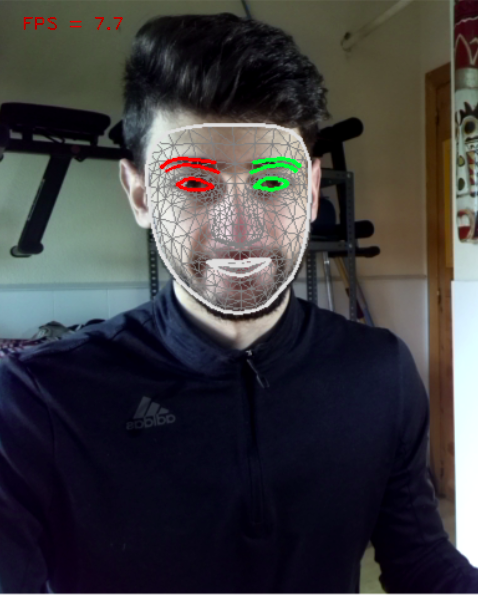
\includegraphics[width=37mm]{figs/mediapipe_buena_luz.png}}
    \subfigure[Malas condiciones de luz]{\includegraphics[width=38mm]{figs/mediapipe_mala_luz.png}}
    \subfigure[Rostros cubiertos]{\includegraphics[width=37mm]{figs/mediapipe_cubiertos.png}}
    \subfigure[Rostros girados]{\includegraphics[width=37mm]{figs/mediapipe_girados.png}}
  \end{center}
\caption{Condiciones en las que se evalúan los fallos de MediaPipe.}
\label{fig:mediapipe_fallos_ejemplos}
\end{figure}

Llegados a este punto, ya habiendo realizado los dos estudios, podemos concluir afirmando que el algoritmo que mejor rendimiento y precisión nos ofrece es el de MediaPipe. Este ha obtenido un rendimiento de 13.28 fps de media, frente a los 8.21 fps de dlib y OpenCV. Además, este último ha obtenido un total de 578 fallos, frente a los 103 fallos de MediaPipe. Por lo tanto, MediaPipe FaceMesh será el algoritmo escogido en este trabajo para obtener la información necesaria de los puntos característicos faciales. Nos brindará información 3D de 468 puntos (Figura \ref{fig:mediapipe_malla}), frente a los 68 que nos hubiera ofrecido dlib.\\

\begin{figure} [h!]
  \begin{center}
    \includegraphics[width=8cm]{figs/canonical_face_model_uv_visualization.png}
  \end{center}
  \captionsetup{justification=centering}
  \caption{Malla facial de MediaPipe de 468 puntos.}
  \label{fig:mediapipe_malla}
\end{figure}

\section{Extracción de información de los puntos faciales}

Tras obtener datos en coordenadas de los puntos faciales característicos de un rostro, debemos tratarlos para que a partir de ellos obtengamos información de las posibles emociones que en ese momento se estén llevando a cabo en el rostro estudiado, y finalmente, crear un dataset con toda esa información que nos permita entrenar modelos de la forma más precisa posible. Esto último es muy importante, porque una de las cosas que determinará la precisión de nuestro modelo, será la existencia de un buen dataset.\\

Retomando la extracción de información, uno de los métodos más usados hasta ahora es la utilización de las distancias entre puntos faciales, tal como se realiza en el artículo \cite{dlib_emotions} (Figura \ref{fig:dlib_foto_articulo}). Por ejemplo, una emoción de \textit{sorpresa} estará caracterizada por poseer grandes distancias entre el labio inferior y la nariz (boca abierta). Sin embargo, esta técnica es propensa a confundir unas emociones con otras, la información de distancias no es suficiente en determinados casos, ya que a veces se puede mantener constante aunque la expresión facial haya cambiado.

\begin{figure} [h!]
  \begin{center}
    \includegraphics[width=7cm]{figs/dlib_foto_articulo.png}
  \end{center}
  \captionsetup{justification=centering}
  \caption{Distancias entre puntos faciales del artículo \cite{dlib_emotions}.}
  \label{fig:dlib_foto_articulo}
\end{figure}

El método usado para extraer información de los puntos faciales, por lo tanto, no será el relatado anteriormente, sino que, se usará un novedoso método propuesto en el artículo \cite{mediapipe_emotions}. Este consiste en construir una \textit{malla emocional} (Figura \ref{fig:malla_emocional}), basada en el Sistema de Codificación Facial o FACS (Facial Action Coding System)\cite{Ekman1978FacialAC}\cite{Ekman1978FacialACManual}, que nos proporcionará información en ángulos de las expresiones faciales.

\begin{figure} [h!]
  \begin{center}
    \includegraphics[width=13cm]{figs/emotional_mesh.png}
  \end{center}
  \captionsetup{justification=centering}
  \caption{\textit{Malla emocional} propuesta en el artículo \cite{mediapipe_emotions}.}
  \label{fig:malla_emocional}
\end{figure}

FACS es un sistema que clasifica movimientos faciales humanos basándose en los cambios producidos en la cara a cargo de los movimientos de los músculos. Estos movimientos son definidos como Unidades de Acción o AUs (Action Units), de los cuales existen hasta 46. En el Cuadro \ref{cuadro:au}, están expuestas las AUs más usadas con sus respectivas descripciones.\\

Además, EMFACS (Emotional Facial Action Coding System) describe emociones simples usando combinaciones de AUs (Cuadro \ref{cuadro:emfacs}). Por lo tanto, sabiendo esto, se puede afirmar que el movimiento de cada uno de esos músculos faciales está relacionado con siete emociones simples, y es por eso, que cada ubicación de los puntos de la \textit{malla emocional} (Figura \ref{fig:malla_emocional}) ha sido elegida de manera que se vea afectada por una AU y de esta manera conseguir un mejor reconocimiento de emociones.\\

\begin{table}[H]
\begin{center}
\begin{tabular}{|c|c|}
     \hline
    \textbf{AU} & \textbf{Descripciones FACS} \\
    \hline
     1 & Interior de las cejas elevado\\ 
     2 & Exterior de las cejas elevado \\ 
     4 & Cejas bajadas \\
     5 & Párpado superior elevado\\
     6 & Mejillas elevadas \\ 
     7 & Párpados tensos \\
     9 & Nariz arrugada \\
     10 & Labio superior elevado \\
     12 & Comisuras de los labios elevados \\ 
     15 & Comisuras de los labios hacia abajo \\
     16 & Labio inferior hacia abajo \\
     17 & Barbilla elevada \\
     20 & Labios apretados y estirados\\
     22 & Labios en forma de \textit{o} \\
     23 & Labios tensos \\
     24 & Labios presionados \\
     25 & Labios separados \\
     26 & Boca abierta (mandíbula caída)\\
     27 & Boca abierta \\
     \hline
 \end{tabular}
 \captionsetup{justification=centering}
\caption{Lista de las Unidades de Acción más usadas y sus respectivas descripciones FACS.}
\label{cuadro:au}
\end{center}
\end{table}

\begin{table}[H]
\begin{center}
\begin{tabular}{|c|c|}
     \hline
    \textbf{Emoción} & \textbf{AU} \\
    \hline
     Felicidad & 6 + 12\\ 
     Tristeza & 1 + 4 + 15 \\ 
     Sorpresa & 1 + 2 + 5 + 26 \\
     Miedo & 1 + 2 + 4 + 5 + 7 + 20 + 26\\
     Enfado & 4 + 5 + 7 + 23 \\ 
     Asco & 9 + 15 + 17 \\
     Desprecio & 12 + 14 \\
     \hline
 \end{tabular}
 \captionsetup{justification=centering}
\caption{Lista de emociones simples en términos de AUs.}
\label{cuadro:emfacs}
\end{center}
\end{table}

Cada uno de los puntos de la \textit{malla emocional} está unido a otros mediante aristas, formando así una malla cerrada de 27 vértices y 38 aristas. Estas aristas forman ángulos entre ellas, y serán estos, los utilizados como información para clasificar emociones. Aprovechando que todas las aristas forman triángulos entre sí (Figura \ref{fig:triangulo}), para calcular los ángulos deseados, se utilizará el teorema del coseno (Ecuación \ref{ec:teorema_coseno}), el cual usa la longitud de las aristas para realizar los cálculos, esto es, la distancia entre los dos puntos que conforman la arista. Esta distancia es calculada mediante distancia euclídea (Ecuación \ref{ec:ecuclidea_puntos}). En forma de código de Python, las funciones que realizarán esta tarea se encuentran en el Código \ref{cod:angulos}.

\begin{figure} [h!]
  \begin{center}
    \includegraphics[width=6cm]{figs/triangulo.png}
  \end{center}
  \captionsetup{justification=centering}
  \caption{Ejemplo de triángulo formado por 2 aristas de la \textit{malla emocional}.}
  \label{fig:triangulo}
\end{figure}

\begin{myequation}[h]
\begin{equation}
\alpha = \arccos{\frac{l_{1}^{2}+l_{3}^{2}-l_{2}^{2}}{2l_{1}l_{3}}}
\nonumber
\label{ec:teorema_coseno}
\end{equation}
\captionsetup{justification=centering}
\caption[Teorema del coseno para calcular el ángulo de la Figura \ref{fig:triangulo}.]{Teorema del coseno para calcular el ángulo de la Figura \ref{fig:triangulo}.}
\end{myequation} 

\begin{myequation}[h]
\begin{equation}
l_{3} = \sqrt{(p_{1x}-p_{2x})^{2}+(p_{1y}-p_{2y})^{2}}
\nonumber
\label{ec:ecuclidea_puntos}
\end{equation}
\captionsetup{justification=centering}
\caption[Distancia euclídea entre los puntos $p_{1}$ y $p_{2}$ de la Figura \ref{fig:triangulo}.]{Distancia euclídea entre los puntos $p_{1}$ y $p_{2}$ de la Figura \ref{fig:triangulo}.}
\end{myequation} 

\begin{code}[h]
\begin{lstlisting}[style=Python]
def distance(self, point1, point2):
    x0 = point1[0]
    y0 = point1[1]
    x1 = point2[0]
    y1 = point2[1]
    return math.sqrt((x0 - x1)**2+(y0 - y1)**2)

def angle(self, point1, point2, point3):
    side1 = self.distance(point2, point3)
    side2 = self.distance(point1, point3)
    side3 = self.distance(point1, point2)
    
    angle = math.degrees(math.acos((side1**2+side3**2-side2**2)/(2*side1*side3)))
    return angle
\end{lstlisting}
\captionsetup{justification=centering}
\caption[Funciones de Python para realizar el cálculo de ángulos\\
de la \textit{malla emocional}.]{Funciones de Python para realizar el cálculo de ángulos\\
de la \textit{malla emocional}.}
\label{cod:angulos}
\end{code}

\section{Generación del dataset}

Siguiendo el esquema de la Figura \ref{fig:metodo}, el paso siguiente a la extracción de información de los puntos faciales es la generación de un dataset (base de datos) con dicha información, para posteriormente entrenar un modelo usando técnicas de Machine Learning, y que este nos permita clasificar emociones. Poseer un buen conjunto de datos es la fase más importante del trabajo, existen proyectos muy buenos que han llegado a fracasar por no poseer un buen dataset. Por lo tanto, hay que dedicar gran parte del tiempo total a la construcción del mismo. Es importante que contenga una buena cantidad de datos y que estos aporten generalidad.\\

La idea a llevar a cabo en este trabajo, es en primer lugar localizar un dataset de imágenes que contenga emociones de distintos sujetos. Seguidamente, tratar cada una de esas imágenes con la \textit{malla emocional} y extraer ángulos de cada una de las emociones. Por último, con esos ángulos se generaría un nuevo dataset, que ya nos serviría para entrenar nuestros modelos. En dicho dataset final, el número de muestras sería el número de fotografías del primer dataset, y el número de características de cada muestra, sería la cantidad de ángulos usados de la \textit{malla emocional}. Un ejemplo de dataset con 224 muestras y cada una de ellas con 21 características se puede encontrar en el Código \ref{cod:ejemplo_dataset}.\\

\begin{code}[h]
\begin{lstlisting}
            X0          X1          X2  ...        X19        X20    y
0    54.288044   37.570711  154.655589  ...  44.625203  63.887010  1.0
1    44.670597   35.229102  148.630240  ...  47.334403  61.278073  1.0
2    46.613914   36.808837  161.148375  ...  57.291823  64.390395  1.0
3    49.404349   47.407905  153.817836  ...  49.880184  61.894869  1.0
4    42.510847   43.626048  146.891826  ...  46.965439  59.971707  1.0
..         ...         ...         ...  ...        ...        ...  ...
220  23.444336   97.667648   88.384186  ...  28.011004  63.905389  7.0
221  24.634940   96.406625   93.413763  ...  28.637606  63.551521  7.0
222  22.425106  105.319774   87.727242  ...  30.811141  61.646881  7.0
223  15.966920  120.968600   60.790043  ...  28.018767  56.442379  7.0
224  19.667632  104.568158   80.332991  ...  29.088510  64.107810  7.0
\end{lstlisting}
\captionsetup{justification=centering}
\caption[Ejemplo de dataset. La primera columna es el número de muestra, \\
la columna \textit{X} son las características, la columna \textit{y} es el tipo de clase.]{Ejemplo de dataset. La primera columna es el número de muestra, \\
la columna \textit{X} son las características, la columna \textit{y} es el tipo de clase.}
\label{cod:ejemplo_dataset}
\end{code}

En cuanto al dataset de imágenes, tras realizar una búsqueda por conseguir las imágenes que mejor se adaptasen a nuestro método, se ha decidido usar \textit{The Extended Cohn-Kanade Dataset (CK+)}\cite{Kanade1}\cite{Kanade2} (Figura \ref{fig:ejemplosCK}). \\

\begin{figure}[h!]
  \begin{center}
    \subcapcentertrue
    \subfigure[Sujeto triste]{\includegraphics[width=50mm]{figs/sujeto_triste.png}}
    \subfigure[Sujeto feliz]{\includegraphics[width=50mm]{figs/sujeto_feliz.png}}
    \subfigure[Sujeto sorprendido]{\includegraphics[width=50mm]{figs/sujeto_sorprendido.png}}
  \end{center}
\captionsetup{justification=centering}
\caption{Ejemplos de imágenes del dataset \textit{The Extended Cohn-Kanade Dataset (CK+)}.}
\label{fig:ejemplosCK}
\end{figure}

Esta base de datos contiene 593 secuencias de imágenes, en las que se muestra un rostro desde una posición neutral hasta la máxima expresión. De esas 593 secuencias, 327 poseen el último \textit{frame} etiquetado con una emoción entre 1 y 7 (1 = anger, 2 = contempt, 3 = disgust, 4 = fear, 5 = happy, 6 = sadness, 7 = surprise). Estos últimos \textit{frames} de esas 327 secuencias, serán los utilizados en este trabajo.\\

CK+ ha sido elegido frente a otro tipo de datasets populares como FER\footnote{FER: \url{https://www.kaggle.com/datasets/msambare/fer2013}}, debido a la alineación de las caras en las imágenes. Bases de datos como la nombrada anteriormente, están enfocadas a ser usadas por CNN (Convolutional Neural Network) y la posición de las caras no influye en el entrenamiento, es más, le aporta más generalidad. Pero para llevar a cabo nuestra técnica, es necesario caras alineadas para obtener información confiable de los ángulos formados por las expresiones faciales. Recordemos que nosostros lo que deseamos es generar un dataset nuevo a partir de otro de imágenes, no utilizar directamente las imágenes como si lo haría una CNN con FER.

\subsection{Cantidad de ángulos a utilizar}

El número de ángulos a utilizar de la \textit{malla emocional}, hará referencia a la cantidad de características que posee nuestro dataset. Es por ello, que se deberá estudiar cuál es la cantidad óptima de los mismos que mejores resultados nos ofrece a la hora de entrenar los modelos.\\

En primer lugar se realizará un estudio para comprobar qué ángulos de toda la malla son más influyentes en las emociones y posteriormente se hará un estudio de simetría con dichos ángulos, para así comprobar si las emociones se pueden considerar simétricas en ambas mitades de un rostro, y de esta manera únicamente utilizar los ángulos de una sola mitad.

\subsubsection{Estudio de influencia}

Tal como se ha comentado anteriormente, realizaremos un estudio para escoger los ángulos más influyentes en cada emoción, esto es, los ángulos que más varían cada vez que se producen dichas expresiones faciales. Para realizar esta prueba, partiremos de todos los ángulos de la parte derecha del rostro (Figura \ref{fig:emotional_mesh_todos_angulos}), y se calculará la variación que existe en cada uno de ellos y para cada una de las emociones de CK+, desde una posición neutral de la cara hasta la máxima expresión.\\

\begin{figure} [h!]
  \begin{center}
    \includegraphics[width=13cm]{figs/emotional_mesh_todos_angulos.png}
  \end{center}
  \captionsetup{justification=centering}
  \caption{Todos los ángulos de la mitad derecha\\
  de la \textit{malla emocional}.}
  \label{fig:emotional_mesh_todos_angulos}
\end{figure}

El método a seguir que nos proporcione esa variación, será calcular la diferencia del ángulo en posición neutral respecto a la posición de la máxima expresión, para ello utilizaremos el Código \ref{cod:angulos_diferencia}. Este, además de calcular la diferencia, evita que aparezcan resultados de otros cuadrantes o negativos. Se realizará este cálculo para cada una de las imágenes de CK+, y los resultados serán las medias calculadas. El resultado del estudio se encuentra en la Figura \ref{fig:estudio_influencia}.\\

\begin{code}[h]
\begin{lstlisting}[language=Python]
def angle_difference(alpha, beta):
    phi = abs(beta-alpha)%360
    if phi > 180:
        return (360 - phi)
    return phi
\end{lstlisting}
\captionsetup{justification=centering}
\caption[Diferencia entre dos ángulos.]{Diferencia entre dos ángulos.}
\label{cod:angulos_diferencia}
\end{code}

Como conclusiones de este estudio, sacamos en claro que los 5 ángulos más influyentes en cada emoción son los mostrados en el Cuadro \ref{cuadro:angulos_5_influyentes}, y que por lo tanto, los ángulos que más varían en total son: 2, 12, 1, 16, 15, 4, 6, 14, 18, 8, 0 y 19.\\

\begin{table}[H]
\begin{center}
\begin{tabular}{|c|c|}
     \hline
    \textbf{Emoción} & \textbf{Ángulos influyentes} \\
    \hline
     Felicidad & 4, 2, 18, 12, 8 \\
     Tristeza & 2, 1, 12, 16, 14 \\
     Sorpresa & 1, 2, 0, 4, 19 \\
     Miedo & 2, 4, 6, 1, 14 \\
     Enfado & 2, 12, 1, 16, 15 \\
     Asco & 12, 16, 2, 15, 1 \\
     Desprecio & 2, 1, 4, 0, 19 \\
     \hline
 \end{tabular}
 \captionsetup{justification=centering}
\caption{Lista de los 5 ángulos más influyentes por cada emoción.}
\label{cuadro:angulos_5_influyentes}
\end{center}
\end{table}

\subsubsection{Estudio de simetría}
Con el afán de descubrir si es posible entrenar a nuestro modelo con sólo ángulos de una mitad del rostro, se va a realizar este estudio de simetría, en el que comprobaremos si las emociones se pueden considerar simétricas para ambos lados de la cara. Para ello, partiremos de los ángulos obtenidos en el estudio anterior (los más influyentes) y generaremos un nuevo mapa que abarque las dos mitades del rostro (Figura \ref{fig:emotional_mesh_2_mitades}).\\

\begin{figure} [h!]
  \begin{center}
    \includegraphics[width=13cm]{figs/emotional_mesh_2_mitades.png}
  \end{center}
  \captionsetup{justification=centering}
  \caption{Mapa de ángulos para realizar el estudio de simetría.}
  \label{fig:emotional_mesh_2_mitades}
\end{figure}

A la hora de estudiar la simetría, calcularemos la variación que existe entre los ángulos del lado izquierdo y del lado derecho, para cada una de las emociones y cada una de las imágenes del dataset CK+. La forma de llevar a cabo este cálculo, será la misma que en el estudio anterior (Código \ref{cod:angulos_diferencia}). Los resultados serán la media de lo obtenido para todas las imágenes, estos se encuentran en la Figura \ref{fig:estudio_simetría}.\\

Finalmente, observando los resultados, podemos considerar que las emociones son simétricas, ya que la mayor variación de media entre el lado izquierdo y derecho ha sido de 5 grados, siendo esta una variación mínima.

\subsubsection{Conclusiones}

Recapitulando, una vez realizados los dos estudios, se procederá ya a generar los dataset. Crearemos dos bases de datos:

\begin{itemize}
    \item Base de datos con todos los ángulos de la parte derecha de la \textit{malla emocional}.
    \item Base de datos con sólo los ángulos más influyentes de la parte derecha de la \textit{malla emocional}.
\end{itemize}

Estos se generan en un fichero csv, en el que cada fila será una muestra, esto es, los datos obtenidos de una imagen de CK+, por lo tanto, poseerá tantas filas como imágenes procesadas. Y cada una de esas filas, tendrá tantas columnas como ángulos calculados en la imagen, y además, una última columna que indicará que tipo de emoción es.
En la siguiente sección se analizará cual de las dos bases de datos nos ofrece mejor rendimiento en el entrenamiento.

\section{Entrenamiento del modelo}
\label{sec:entrenamiento}

Se va a realizar el entrenamiento con tres algoritmos de clasificación diferentes y se compararan los resultados de cada uno de ellos. Los algoritmos a utilizar serán KNN, SVM y MLP. Además, se hará uso de PCA para mejorar la precisión de la detección de emociones. Se estudiará si ofrece mejor resultado el dataset con ángulos reducidos o el que posee todos los ángulos, pero reduciendo estos a través de PCA.\\

Cada uno de los algoritmos posee unos parámetros a optimizar en la fase de entrenamiento, nuestro labor será encontrar aquellos valores que proporcionen más precisión al modelo sin llegar a sobreentrenarlo. En caso de KNN se deberá encontrar el número de vecinos óptimo (k), para SVM el parámetro de regulación óptimo (C) y para MLP el número de capas ocultas y neuronas óptimas. Los demás parámetros de configuración como la función de activación en MLP o el algoritmo para calcular distancias en KNN, se dejarán por defecto tal como los ofrece Scikit-Learn, son los que mejores resultados ofrecen.\\

A la hora de conocer la precisión obtenida durante el entrenamiento, existen varios valores que puntúan el desempeño del modelo:

\begin{itemize}
    \item \textit{Precision.} De las predicciones que ha realizado, indica que porcentaje son correctas.
    \item \textit{Recall.} De los datos, indica que porcentaje están bien predichos.
    \item \textit{F1-Score.} Hace referencia a la media ponderada entre \textit{Precision} y \textit{Recall}.
    \item \textit{Accuracy.} La suma de los aciertos entre el número total de muestras, osea el porcentaje de acierto.
\end{itemize}

Y por último, para evitar el sobreentrenamiento y generalizar los modelos, se hará uso de la validación cruzada K-Fold. Este método nos permitirá usar todos los datos como test y todos los datos como entrenamiento. Esto se consigue gracias a que el algoritmo divide el conjunto de datos en \textit{K pliegues}, y uno de ellos es dedicado a datos de test. Entonces, por cada iteración este conjunto de test se va desplazando a la derecha. En la Figura \ref{fig:kfolf_explicacion}, encontramos un ejemplo de 4 \textit{pliegues}.\\

\begin{figure} [h!]
  \begin{center}
    \includegraphics[width=10cm]{figs/KFold_explanation.png}
  \end{center}
  \captionsetup{justification=centering}
  \caption{Ejemplo de división de la base de datos \\
  en 4 \textit{pliegues} usando KFold.}
  \label{fig:kfolf_explicacion}
\end{figure}

La clase con menos datos del dataset CK+, tiene una cantidad de 28. Por lo tanto, se usarán 4 \textit{pliegues} para KFold, de esta manera aseguramos 8 datos de esa clase en cada pliegue. Al tener una base de datos desequilibrada, esto es, que no tiene el mismo número de muestras para todas las clases, debemos usar KFoldStratified, que nos asegura poseer siempre el mismo porcentaje de muestras de cada clase en todos los pliegues.\\

KFoldStratified por lo tanto, nos servirá para encontrar los parámetros óptimos de cada algoritmo. Por ejemplo, para KNN probaremos cada una de las \textit{k} (vecinos) posibles en cada una de las iteraciones. El resultado sería una matriz con el \textit{Accuracy} para cada una de las \textit{k} en cada una de las iteraciones. Finalmente, se calcularía la media de todas las iteraciones y escogeríamos la \textit{k} que más \textit{Accuracy} de media haya obtenido. Esto sería el número de vecinos óptimo. Un ejemplo con 4 valores de vecinos se muestra en la Figura \ref{fig:kfold_KNN}.\\

\begin{figure} [h!]
  \begin{center}
    \includegraphics[width=13cm]{figs/KFold_KNN.png}
  \end{center}
  \captionsetup{justification=centering}
  \caption{Ejemplo de búsqueda del número de vecinos\\
  óptimo para KNN usando KFold.}
  \label{fig:kfold_KNN}
\end{figure}

Para el caso en el que además usemos PCA para reducir el número de características (componentes), debemos encontrar además el número óptimo de las mismas. Entonces, en vez de tener una matriz de 2 dimensiones, pasamos a trabajar con una matriz de 3 dimensiones. Se puede ver un ejemplo en la Figura \ref{fig:kfold_KNN_PCA}. Al igual que en el caso anterior, la combinación óptima de vecinos y componentes de PCA, será la que haya obtenido mejor puntuación de media.\\

\begin{figure} [h!]
  \begin{center}
    \includegraphics[width=16cm]{figs/KFold_KNN_PCA.png}
  \end{center}
  \captionsetup{justification=centering}
  \caption{Ejemplo de búsqueda del número de vecinos\\
  óptimo para KNN y el número de componentes\\
  óptimo a reducir por PCA usando KFold.}
  \label{fig:kfold_KNN_PCA}
\end{figure}

\subsection{Dataset de ángulos influyentes}

Los parámetros óptimos, para el dataset de ángulos influyentes, tras realizar su búsqueda usando validación cruzada KFoldStratified de 4 \textit{pliegues}, se encuentran en el Cuadro \ref{cuadro:parametros_dataset1}. Para KNN se ha probado con valores de k impares entre 1 y 13 incluidos, para SVM con valores de C entre 1 y 999 (saltos de 10 en 10) y para MLP se ha probado con 1 capa oculta de neuronas entre 5 y 24 incluidos, no ha sido necesario añadir más capas.\\

\begin{table}[H]
\begin{center}
\begin{tabular}{|c|c|}
     \hline
    \textbf{Clasificador} & \textbf{Parámetros} \\
    \hline
     KNN & \verb|k = 11| \\
     SVM & \verb|C = 11| \\
     MLP & \verb|hidden_layer_sizes = (19)|\\
     \hline
 \end{tabular}
 \captionsetup{justification=centering}
\caption{Parámetros óptimos para cada uno de los clasificadores\\
entrenando el dataset de ángulos influyentes.}
\label{cuadro:parametros_dataset1}
\end{center}
\end{table}

Finalmente, los resultados obtenidos en el entrenamiento para dicho dataset y los parámetros, se encuentran en el Cuadro \ref{cuadro:resultados_dataset1}. Estos han sido calculados también mediante validación cruzada KFoldStratified de 4 \textit{pliegues}, y se muestra la media de todas las iteraciones.\\

\begin{table}[H]
\begin{center}
\begin{tabular}{|c|c|c|c|c|}
     \hline
    \textbf{Clasificador} & \textbf{Accuracy} & \textbf{Precision} & \textbf{Recall} & \textbf{F1-score}\\
    \hline
     KNN & 0.82 & 0.76 & 0.74 & 0.74\\
     SVM & 0.84 & 0.79 & 0.78 & 0.77\\
     MLP & 0.82 & 0.78 & 0.78 & 0.77\\
     \hline
 \end{tabular}
 \captionsetup{justification=centering}
\caption{Resultados de precisión de los clasificadores con\\
el dataset de ángulos influyentes.}
\label{cuadro:resultados_dataset1}
\end{center}
\end{table}

\subsection{Dataset de todos los ángulos}

Tal como se ha comentado en la Sección \ref{sec:entrenamiento}, como este dataset posee todos los ángulos de una mitad del rostro, se usará PCA para hacer la reducción de características (ángulos). El valor óptimo de características a reducir y los parámetros para cada clasificador, tras realizar su búsqueda usando validación cruzada KFoldStratified de 4 \textit{pliegues}, se encuentran en el Cuadro \ref{cuadro:parametros_dataset2}. Para hacer la reducción con PCA, se ha probado con un número de componentes entre 2 y 20 incluidos, para KNN se ha probado con valores de k impares entre 1 y 13 incluidos, para SVM con valores de C entre 1 y 999 (saltos de 10 en 10) y para MLP se ha probado con 1 capa oculta de neuronas entre 5 y 24 incluidos, no ha sido necesario añadir más capas.\\

\begin{table}[H]
\begin{center}
\begin{tabular}{|c|c|}
     \hline
    \textbf{Clasificador y PCA} & \textbf{Parámetros} \\
    \hline
     KNN y PCA & \verb|k = 11|, \verb|n_components = 17|\\
     SVM y PCA & \verb|C = 11|, \verb|n_components = 7|\\
     MLP y PCA & \verb|hidden_layer_sizes = (12)|, \verb|n_components = 11|\\
     \hline
 \end{tabular}
 \captionsetup{justification=centering}
\caption{Parámetros óptimos para cada uno de los clasificadores\\
entrenando el dataset de todos los ángulos.}
\label{cuadro:parametros_dataset2}
\end{center}
\end{table}

Finalmente, los resultados obtenidos en el entrenamiento para dicho dataset (reduciendo el número de características con PCA) y los parámetros óptimos, se encuentran en el Cuadro \ref{cuadro:resultados_dataset2}. Estos resultados de precisión han sido calculados también mediante validación cruzada KFoldStratified de 4 \textit{pliegues}, y se muestra la media de todas las iteraciones.\\

\begin{table}[H]
\begin{center}
\begin{tabular}{|c|c|c|c|c|}
     \hline
    \textbf{Clasificador} & \textbf{Accuracy} & \textbf{Precision} & \textbf{Recall} & \textbf{F1-score}\\
    \hline
     KNN & 0.83 & 0.79 & 0.75 & 0.75\\
     SVM & 0.84 & 0.80 & 0.77 & 0.78\\
     MLP & 0.84 & 0.81 & 0.80 & 0.80\\
     \hline
 \end{tabular}
 \captionsetup{justification=centering}
\caption{Resultados de precisión de los clasificadores con\\
el dataset de todos los ángulos, reducido con PCA.}
\label{cuadro:resultados_dataset2}
\end{center}
\end{table}

\subsection{Conclusiones y propuesta de mejora}
Los resultados obtenidos para cada uno de los datasets son bastante similares, aunque un poco superiores para el dataset de todos los ángulos con reducción de características usando PCA, sobre todo si observamos \textit{Precision}, \textit{Recall} y \textit{F1-score}. En cuanto a los resultados obtenidos por cada clasificador, también son muy similares y sería muy complicado decantarse por uno sólo.\\

Sin embargo, en general no son resultados demasiado buenos y la herramienta robótica construida a partir de estos modelos no sería muy robusta. Sobre todo si observamos los resultados de cada una de las clases por separado, por ejemplo los arrojados por SVM usando el dataset de todos los ángulos (Cuadro \ref{cuadro:resultados_SVM}). En dichos resultados, podemos observar que clases como ---por ejemplo--- la de \textit{Desprecio} o la de \textit{Enfado} han obtenido puntuaciones realmente malas, incluso por debajo del 50\% en algún caso. Por lo tanto, esto nos lleva a pensar que nuestro sistema no va a dar buen rendimiento a la hora de detectar todas las emociones, aunque de media si que tenga una puntuación aceptable.\\

\begin{table}
\begin{minipage}{0.48\linewidth}
\centering
\begin{adjustbox}{max width=\textwidth}
\begin{tabular}{|c|c|c|c|}
\hline
\textbf{Clase} & \textbf{Precision} & \textbf{Recall} & \textbf{F1-score}\\
\hline
     Enfado & 0.67 & 0.50 & 0.57\\
     Desprecio & 0.67 & 0.50 & 0.57\\
     Asco & 0.76 & 0.87 & 0.81\\
     Miedo & 0.67 & 1.00 & 0.80\\
     Felicidad & 0.94 & 0.94 & 0.94\\
     Tristeza & 0.83 & 0.71 & 0.77\\
     Sorpresa & 0.95 & 0.95 & 0.95\\
\hline
\end{tabular}
\end{adjustbox}
\vspace{0.5cm}

\begin{adjustbox}{max width=\textwidth}
\begin{tabular}{|c|c|c|c|}
\hline
\textbf{Clase} & \textbf{Precision} & \textbf{Recall} & \textbf{F1-score}\\
\hline
     Enfado & 0.75 & 0.82 & 0.78\\
     Desprecio & 0.67 & 0.80 & 0.73\\
     Asco & 0.82 & 0.93 & 0.87\\
     Miedo & 0.80 & 0.67 & 0.73\\
     Felicidad & 0.94 & 0.94 & 0.94\\
     Tristeza & 1.00 & 0.57 & 0.73\\
     Sorpresa & 0.95 & 0.95 & 0.95\\
\hline
\end{tabular}
\end{adjustbox}
\end{minipage}\hfill
\begin{minipage}{0.48\linewidth}
\centering
\begin{adjustbox}{max width=\textwidth}
\begin{tabular}{|c|c|c|c|}
\hline
\textbf{Clase} & \textbf{Precision} & \textbf{Recall} & \textbf{F1-score}\\
\hline
     Enfado & 0.71 & 0.45 & 0.56\\
     Desprecio & 0.57 & 0.80 & 0.67\\
     Asco & 0.76 & 0.93 & 0.84\\
     Miedo & 1.00 & 0.71 & 0.83\\
     Felicidad & 0.85 & 1.00 & 0.92\\
     Tristeza & 0.83 & 0.71 & 0.77\\
     Sorpresa & 1.00 & 0.95 & 0.98\\
\hline
\end{tabular}
\end{adjustbox}
\vspace{0.5cm}

\begin{adjustbox}{max width=\textwidth}
\begin{tabular}{|c|c|c|c|}
\hline
\textbf{Clase} & \textbf{Precision} & \textbf{Recall} & \textbf{F1-score}\\
\hline
     Enfado & 0.67 & 0.55 & 0.60\\
     Desprecio & 0.50 & 0.25 & 0.33\\
     Asco & 0.67 & 0.80 & 0.73\\
     Miedo & 1.00 & 0.67 & 0.80\\
     Felicidad & 1.00 & 1.00 & 1.00\\
     Tristeza & 0.50 & 0.71 & 0.59\\
     Sorpresa & 1.00 & 1.00 & 1.00\\
\hline
\end{tabular}
\end{adjustbox}
\end{minipage}
\captionsetup{justification=centering}
\caption{Resultados del entrenamiento con SVM en cada una\\
de las 4 iteraciones de KFoldStratified, usando el dataset\\
de todos los ángulos.}
\label{cuadro:resultados_SVM}
\end{table}

Esta mala clasificación de algunas emociones, se debe a la gran similitud que existe entre varias. Esto provoca que geométricamente sean prácticamente indiferenciables, y por lo tanto, es complicado que los algoritmos sepan clasificarlas correctamente. Si observamos el estudio de ángulos influyentes en cada emoción (Figura \ref{fig:estudio_influencia}), podemos ver que ---por ejemplo--- las emociones \textit{sorpresa} y \textit{desprecio} poseen exactamente los mismos 5 ángulos influyentes, o las emociones \textit{enfado} y \textit{asco} que también poseen los mismos 5 (Cuadro \ref{cuadro:angulos_5_influyentes}). Esto dificulta muchísimo la tarea de clasificación.\\

Por lo tanto, se propone eliminar las emociones que estén interceptando con otras, y de esta manera, aumentar la robustez de nuestra futura herramienta, consiguiendo mayor precisión en nuestro modelo. Las emociones que se elegirán, son las siguientes: \textit{felicidad}, \textit{tristeza}, \textit{sorpresa} y \textit{enfado}. Son las 4 emociones simples más generales, y además, se diferencian geométricamente unas de otras.\\

Se usará el dataset con todos los ángulos (reducido con PCA), ya que es con el que se ha obtenido una precisión ligeramente superior, pero esta vez únicamente con las clases: \textit{felicidad}, \textit{tristeza}, \textit{sorpresa} y \textit{enfado}. Utilizando la técnica de validación cruzada, de la misma manera que en las secciones anteriores, los parámetros óptimos encontrados para cada uno de los algoritmos se encuentran en el Cuadro \ref{cuadro:parametros_dataset3}. Y los resultados del entrenamiento con dichos parámetros óptimos, en el Cuadro \ref{cuadro:resultados_dataset3}.\\

\begin{table}[H]
\begin{center}
\begin{tabular}{|c|c|}
     \hline
    \textbf{Clasificador y PCA} & \textbf{Parámetros} \\
    \hline
     KNN y PCA & \verb|k = 7|, \verb|n_components = 11|\\
     SVM y PCA & \verb|C = 21|, \verb|n_components = 11|\\
     MLP y PCA & \verb|hidden_layer_sizes = (17)|, \verb|n_components = 11|\\
     \hline
 \end{tabular}
 \captionsetup{justification=centering}
\caption{Parámetros óptimos para cada uno de los clasificadores\\
entrenando con el dataset de todos los ángulos (\textit{felicidad}, \\
\textit{tristeza}, \textit{sorpresa} y \textit{enfado}), reducido con PCA.}
\label{cuadro:parametros_dataset3}
\end{center}
\end{table}

\begin{table}[H]
\begin{center}
\begin{tabular}{|c|c|c|c|c|}
     \hline
    \textbf{Clasificador} & \textbf{Accuracy} & \textbf{Precision} & \textbf{Recall} & \textbf{F1-score}\\
    \hline
     KNN & 0.95 & 0.93 & 0.94 & 0.92\\
     SVM & 0.95 & 0.93 & 0.92 & 0.92\\
     MLP & 0.95 & 0.95 & 0.93 & 0.93\\
     \hline
 \end{tabular}
 \captionsetup{justification=centering}
\caption{Resultados de precisión de los clasificadores con\\
el dataset de todos los ángulos (\textit{felicidad}, \textit{tristeza}, \\
\textit{sorpresa} y \textit{enfado}), reducido con PCA.}
\label{cuadro:resultados_dataset3}
\end{center}
\end{table}

Como conclusiones finales, observamos que en este último entrenamiento ya si que realmente hemos obtenido unos resultados muy buenos para los tres clasificadores, con un porcentaje de acierto medio del 95\%. Además, consultando por separado los resultados de cada una de las clases en cada una de las iteraciones de la validación cruzada, afirmamos también que esta vez ya ninguna emoción tiene malos resultados. Por ejemplo, para el entrenamiento con KNN en el Cuadro \ref{cuadro:resultados_KNN}.\\

\begin{table}
\begin{minipage}{0.48\linewidth}
\centering
\begin{adjustbox}{max width=\textwidth}
\begin{tabular}{|c|c|c|c|}
\hline
\textbf{Clase} & \textbf{Precision} & \textbf{Recall} & \textbf{F1-score}\\
\hline
     Enfado & 0.88 & 0.58 & 0.70\\
     Felicidad & 0.94 & 1.00 & 0.97\\
     Tristeza & 0.58 & 1.00 & 0.74\\
     Sorpresa & 1.00 & 0.90 & 0.95\\
\hline
\end{tabular}
\end{adjustbox}
\vspace{0.5cm}

\begin{adjustbox}{max width=\textwidth}
\begin{tabular}{|c|c|c|c|}
\hline
\textbf{Clase} & \textbf{Precision} & \textbf{Recall} & \textbf{F1-score}\\
\hline
     Enfado & 1.00 & 1.00 & 1.00\\
     Felicidad & 1.00 & 1.00 & 1.00\\
     Tristeza & 1.00 & 1.00 & 1.00\\
     Sorpresa & 1.00 & 1.00 & 1.00\\
\hline
\end{tabular}
\end{adjustbox}
\end{minipage}\hfill
\begin{minipage}{0.48\linewidth}
\centering
\begin{adjustbox}{max width=\textwidth}
\begin{tabular}{|c|c|c|c|}
\hline
\textbf{Clase} & \textbf{Precision} & \textbf{Recall} & \textbf{F1-score}\\
\hline
     Enfado & 1.00 & 0.82 & 0.90\\
     Felicidad & 1.00 & 1.00 & 1.00\\
     Tristeza & 0.78 & 1.00 & 0.88\\
     Sorpresa & 1.00 & 1.00 & 1.00\\
\hline
\end{tabular}
\end{adjustbox}
\vspace{0.5cm}

\begin{adjustbox}{max width=\textwidth}
\begin{tabular}{|c|c|c|c|}
\hline
\textbf{Clase} & \textbf{Precision} & \textbf{Recall} & \textbf{F1-score}\\
\hline
     Enfado & 0.90 & 0.82 & 0.86\\
     Felicidad & 1.00 & 1.00 & 1.00\\
     Tristeza & 0.75 & 0.86 & 0.80\\
     Sorpresa & 1.00 & 1.00 & 1.00\\
\hline
\end{tabular}
\end{adjustbox}
\end{minipage}
\captionsetup{justification=centering}
\caption{Resultados del entrenamiento con KNN en cada una\\
de las 4 iteraciones de KFoldStratified, usando el dataset\\
de todos los ángulos (\textit{felicidad}, \textit{tristeza}, \\
\textit{sorpresa} y \textit{enfado}), reducido con PCA.}
\label{cuadro:resultados_KNN}
\end{table}

Los modelos entrenados, serán guardados en ficheros con formato pkl usando el módulo \textit{pickle} de Python. De esta manera, pueden ser cargados en cualquier otro programa y realizar predicciones con ellos usando el método \verb|predict()|. A este último, se le deberán introducir los ángulos del rostro a clasificar, y te devolverá la clase predicha.

\section{Integración del sistema en ROS}

El último paso a llevar a cabo en este trabajo, es integrar el sistema de detección de emociones en ROS para facilitar su uso en un sistema robótico. Con esto, se pretende crear una herramienta que abstraiga al desarrollador robótico del código de nuestro sistema, y que por lo tanto, a través de \textit{topics} de ROS obtenga todos los datos detectados por el sistema de manera fácil.\\

En esta sección, se comenzará explicando cual ha sido el proceso llevado a cabo para instalar ROS bajo Raspberry Pi OS, se comentará la estructura del paquete y del código ROS desarrollado, y por último, se hará una explicación de su funcionamiento, así cómo, comentando aspectos de su rendimiento.

\subsection{Instalación de ROS en Raspberry}

El objetivo principal es instalar ROS2, pero no existe ninguna versión de este compatible con 32-bit, y la versión de 64-bit de Raspberry Pi OS, a fecha de hoy, no tiene total compatibilidad con todas las librerías usadas en este trabajo. Igualmente, se ha intentado instalar ROS2 en Raspberry Pi OS de 64-bit, pero no ha resultado satisfactorio, hay paquetes que no son compatibles con un procesador ARM.\\

De forma alternativa, se instalará ROS Noetic, ya que existe una versión del mismo para Debian Buster, y la versión de Raspberry Pi OS usada en este trabajo está basada en Debian Buster. Sin embargo, no se puede hacer la instalación de la forma tradicional a través de \textit{apt}, porque dicha versión de ROS tiene soporte nivel 3 \footnote{Nivel 3: no existen archivos binarios, el usuario debe compilar el código desde la fuente}. Los pasos a seguir para su instalación son los siguientes\footnote{\url{https://varhowto.com/install-ros-noetic-raspberry-pi-4/}}:\\

\noindent
Añadimos el repositorio oficial de ROS para Debian.
\begin{listing}[style=consola, numbers=none]
$ sudo sh -c 'echo "deb http://packages.ros.org/ros/ubuntu buster main" > /etc/apt/sources.list.d/ros-noetic.list'
\end{listing}

\noindent
Agregamos la clave de ROS, para asegurarnos de que instalamos paquetes de ROS autenticados.
\begin{listing}[style=consola, numbers=none]
$ sudo apt-key adv --keyserver 'hkp://keyserver.ubuntu.com:80' --recv-key C1CF6E31E6BADE8868B172B4F42ED6FBAB17C654
\end{listing}

\noindent
Actualizamos los repositorios del sistema.
\begin{listing}[style=consola, numbers=none]
$ sudo apt-get update
\end{listing}

\noindent
Instalamos las dependencias de compilación.
\begin{listing}[style=consola, numbers=none]
$ sudo apt-get install -y python-rosdep python-rosinstall-generator python-wstool python-rosinstall build-essential cmake
\end{listing}

\noindent
Inicializamos \verb|rosdep|.
\begin{listing}[style=consola, numbers=none]
$ sudo rosdep init
$ rosdep update
\end{listing}

\noindent
Creamos un espacio de trabajo de ROS.
\begin{listing}[style=consola, numbers=none]
$ mkdir ~/ros_catkin_ws 
$ cd ~/ros_catkin_ws
\end{listing}

\noindent
Usamos \verb|rosinstall_generator| para generar una lista de dependencias de Noetic para la variante \verb|ros_comm|, porque los tradicionales \verb|desktop-full| o \verb|desktop| no son compatibles y la Raspberry no posee la suficiente memoria como para compilar rviz.
\begin{listing}[style=consola, numbers=none]
$ rosinstall_generator ros_comm --rosdistro noetic --deps --wet-only --tar > noetic-ros_comm-wet.rosinstall
\end{listing}

\noindent
Usamos \verb|wstool| para obtener todos los repositorios.
\begin{listing}[style=consola, numbers=none]
$ wstool init src noetic-ros_comm-wet.rosinstall
\end{listing}

\noindent
Instalamos dependencias usando \verb|rosdep|.
\begin{listing}[style=consola, numbers=none]
$ rosdep install -y --from-paths src --ignore-src --rosdistro noetic -r --os=debian:buster
\end{listing}

\noindent
Por último, antes de compilar, aumentamos el espacio de \verb|swap|, que se usará cuando se agote la memoria física en la Raspberry. Primero desactivamos la memoria \verb|swap|.
\begin{listing}[style=consola, numbers=none]
$ sudo dphys-swapfile swapoff
\end{listing}

\noindent
Editamos el archivo \verb|/etc/dphys-swapfile|, cambiando \verb|CONF_SWAPSIZE=100| por \verb|CONF_SWAPSIZE=1024|. Y volvemos a configurar y activar la \verb|swap|.
\begin{listing}[style=consola, numbers=none]
$ sudo dphys-swapfile setup
$ sudo dphys-swapfile swapon
\end{listing}

\noindent
Procedemos a realizar la compilación, todo se instalará en \verb|/opt/ros/noetic|.
\begin{listing}[style=consola, numbers=none]
$ sudo src/catkin/bin/catkin_make_isolated --install -DCMAKE_BUILD_TYPE=Release --install-space /opt/ros/noetic -j1 -DPYTHON_EXECUTABLE=/usr/bin/python3
\end{listing}

\subsection{Estructura ROS y código desarrollado}

Se ha desarrollado un paquete llamado \verb|emotion_detection_ros|\footnote{\url{https://github.com/jmrtzma/emotion_detection_ros}}. Un esquema general de su funcionamiento se puede ver en la Figura \ref{fig:esquema_paquete_ROS}.\\

\begin{figure} [h!]
  \begin{center}
    \includegraphics[width=15cm]{figs/paquete_ros.png}
  \end{center}
  \captionsetup{justification=centering}
  \caption{Esquema general del paquete de ROS.}
  \label{fig:esquema_paquete_ROS}
\end{figure}

El nodo \verb|emotion_detection| recibe los \textit{frames} de una cámara a través de un \textit{topic} que maneja mensajes del tipo \verb|sensor_msgs/CompressedImage|, este nodo se encargará de hacer todo el procesamiento, y a través de otro tópic que maneja mensajes del tipo \verb|emotion_detection_ros_msgs/BoundingBoxes|, envía una lista de \verb|emotion_detection_ros_msgs/BoundingBox|. Cada uno de estos últimos mensajes contiene la información de cada emoción detectada: un \textit{float64} con la probabilidad de la predicción, cuatro \textit{int64} con las coordenadas del bounding box que rodea la emoción detectada, y un \textit{string} con la emoción detectada.

\subsubsection{Parámetros de configuración}

El paquete posee un directorio \textit{config} en el que se encuentran dos ficheros de configuración. Estos son de formato \textit{yaml}, y sirven para personalizar parámetros del código sin necesidad de editar el mismo.\\

El fichero \verb|model.yaml| (Código \ref{cod:model}), nos permite cambiar el algoritmo que usará nuestro sistema para realizar la clasificación de emociones (KNN, SVM o MLP) y elegir el número máximo de caras que deseamos que se detecten. Este último nos permite controlar el rendimiento ofrecido, ya que por cada cara nueva que se esté detectando, los FPS se reducen.\\

\begin{code}[h]
\begin{lstlisting}
model:

  algorithm: KNN
  max_num_faces: 1
\end{lstlisting}
\captionsetup{justification=centering}
\caption[Fichero de configuración model.yaml.]{Fichero de configuración model.yaml.}
\label{cod:model}
\end{code}

El fichero \verb|ros.yaml| (Código \ref{cod:ros_yaml}), nos permite cambiar los nombres de los \textit{topics} usados, además de algunos parámetros de configuración de los publicadores y suscriptores. Por último, podemos elegir si deseamos que se muestre el visualizador o no, así como, el delay entre los \textit{frames} mostrados en este.

\begin{code}[h]
\begin{lstlisting}
subscribers:

  camera_reading:
    topic: /raspicam_node/image/compressed
    queue_size: 1

publishers:

  bounding_boxes:
      topic: /emotion_detection_ros/bounding_boxes
      queue_size: 1
      latch: False

image_view:

  enable: True
  wait_key_delay: 1
\end{lstlisting}
\captionsetup{justification=centering}
\caption[Fichero de configuración ros.yaml.]{Fichero de configuración ros.yaml.}
\label{cod:ros_yaml}
\end{code}

\subsubsection{Ficheros de código}

El nodo principal se encuentra en el fichero \verb|emotion_detection_node.py| del directorio \verb|scripts|. Este posee dos \textit{threads}. El principal del programa se encarga de recibir los \textit{frames} a través de un subscriptor, y el otro \textit{thread} se encarga de realizar el procesamiento de los frames, esto es, realizar las predicciones, dibujar el bounding box, dibujar el valor de FPS, y además publicar los datos obtenidos en el \textit{topic} correspondiente. Se ha organizado de esta manera para conseguir un mayor rendimiento, ya que realizando el procesamiento en un \textit{thread} distinto al principal, no se tratarán estrictamente todos los frames, lo que impulsará considerablemente el valor de FPS del sistema.\\

Las tareas del nodo principal, están repartidas en diferentes clases que se encuentran en el directorio \verb|src|:

\begin{itemize}
    \item \verb|EmotionalMesh|. Encapsula cada \textit{malla emocional} detectada. Recibe como entrada las coordenadas de los puntos faciales detectados por MediaPipe FaceMesh, y con ello, forma la \textit{malla emocional} y calcula todos los ángulos.
    
    \item \verb|EmotionalMeshDetection|. Se encarga de detectar los puntos faciales de la cara usando MediaPipe FaceMesh, y con ello, genera una lista de objetos \verb|EmotionalMesh|, esto es, una lista con las \textit{mallas emocionales} de las caras detectadas en el \textit{frame}.
    
    \item \verb|Emotion|. Encapsula los datos de cada predicción realizada, esto es, el nombre de la emoción, la probabilidad, la etiqueta que se mostrará por pantalla que contiene el nombre de la emoción y la probabilidad, y las coordenadas del bounding box que rodea esa cara.
    
    \item \verb|EmotionPredictor|. Se encarga de realizar las predicciones en los frames usando el modelo entrenado y los objetos \verb|EmotionalMesh|. Genera una lista de objetos \verb|Emotion| con los datos de las predicciones.
\end{itemize}

\subsection{Uso y rendimiento}

Gracias a que el sistema está integrado en ROS y la comunicación se produce a través de \textit{topics}, se podría usar cualquier cámara que publique \textit{frames} en el \textit{topic} necesario. Sin embargo, se recomienda usar la Raspberry Pi Camera V2.1, ya que ha sido la cámara usada en este trabajo.\\

Para usar dicha cámara en nuestro entorno ROS, se ha hecho uso del paquete \verb|raspicam_node| \footnote{\url{https://github.com/UbiquityRobotics/raspicam_node}}. Este se encarga de leer \textit{frames} de la Raspberry Pi Camera de forma eficiente y publicarlos en el \textit{topic} \verb|/raspicam_node/image/compressed|.\\

Con los paquetes \verb|emotion_detection_ros| y \verb|raspicam_node| compilados en el \textit{workspace} de ROS. Los pasos a seguir para poner en marcha el sistema son los siguientes:\\

\noindent
Lanzamos el launcher de la cámara.
\begin{listing}[style=consola, numbers=none]
$ roslaunch raspicam_node camerav2_410x308_30fps.launch
\end{listing}

\noindent
Lanzamos el sistema de detección de emociones
\begin{listing}[style=consola, numbers=none]
$ roslaunch emotion_detection_ros emotion_detection_ros.launch
\end{listing}

Tras lanzar el sistema, se abrirá una ventana gráfica en la que se mostrarán los \textit{frames}, en los cuales aparecerán dibujados los bounding boxes con sus respectivas etiquetas mostrando la predicción. Además, en la esquina superior izquierda se expondrá el valor de FPS del sistema (Figura \ref{fig:ventana_grafica_1_cara}).\\

\begin{figure}[h!]
  \begin{center}
  \subcapcentertrue
    \subfigure[Predicción de felicidad]{\includegraphics[width=75mm]{figs/prediccion_happy.png}}
    \subfigure[Predicción de enfado]{\includegraphics[width=75mm]{figs/prediccion_anger.png}}
    \subfigure[Predicción de tristeza]{\includegraphics[width=75mm]{figs/prediccion_sadness.png}}
    \subfigure[Predicción de sorpresa]{\includegraphics[width=75mm]{figs/prediccion_surprise.png}}
  \end{center}
 \captionsetup{justification=centering}
\caption{Ejemplos de la ventana gráfica del sistema de detección\\
de emociones funcionando en ROS.}
\label{fig:ventana_grafica_1_cara}
\end{figure}

Otro ejemplo, esta vez detectando dos caras, se encuentra en la Figura \ref{fig:ventana_grafica_2_caras}. Y si ejecutamos el comando \verb|rostopic echo /emotion_detection_ros/bounding_boxes|, podemos observar como la información detectada se está publicando en dicho \textit{topic} (Figura \ref{fig:ejemplo_salida_topic}).\\

\begin{figure} [h!]
  \begin{center}
    \includegraphics[width=75mm]{figs/prediccion_happy_surprise.png}
  \end{center}
  \captionsetup{justification=centering}
  \caption{Ejemplo del sistema en ROS detectando las\\
  emociones de dos caras.}
  \label{fig:ventana_grafica_2_caras}
\end{figure}

\begin{figure} [h!]
  \begin{center}
    \includegraphics[width=13cm]{figs/salida_topic.png}
  \end{center}
  \captionsetup{justification=centering}
  \caption{Ejemplo de información publicada en el \textit{topic}\\
  /emotion\_detection\_ros/bounding\_boxes.}
  \label{fig:ejemplo_salida_topic}
\end{figure}

En cuanto al rendimiento general del sistema, se ha realizado un estudio del valor de FPS arrojado dependiendo del número de caras detectadas. Se han realizado tres pruebas, en cada una de ellas modificando el parámetro de configuración \verb|max_num_faces| del fichero \verb|model.yaml|, de esta manera se ha probado el sistema con hasta tres caras. Los resultados se encuentran en los Cuadros \ref{cuadro:rendimiento_ros_1}, \ref{cuadro:rendimiento_ros_2} y \ref{cuadro:rendimiento_ros_3}.\\

\begin{table}[H]
\begin{center}
\begin{adjustbox}{max width=\textwidth}
\begin{tabular}{|c|c|c|c|}
     \hline
    \textbf{Caras detectadas} & \textbf{Media de FPS} & \textbf{Valor máximo de FPS} & \textbf{Valor mínimo de FPS}\\
    \hline
     1 & 13.18 & 15.13 & 11.04\\
     \hline
 \end{tabular}
 \end{adjustbox}
 \captionsetup{justification=centering}
\caption{Rendimiento del sistema en ROS con max\_num\_faces: 1.}
\label{cuadro:rendimiento_ros_1}
\end{center}
\end{table}

\begin{table}[H]
\begin{center}
\begin{adjustbox}{max width=\textwidth}
\begin{tabular}{|c|c|c|c|}
     \hline
    \textbf{Caras detectadas} & \textbf{Media de FPS} & \textbf{Valor máximo de FPS} & \textbf{Valor mínimo de FPS}\\
    \hline
     1 & 11.11 & 11.97 & 9.18\\
     2 & 7.53 & 8.35 & 6.96\\
     \hline
 \end{tabular}
 \end{adjustbox}
 \captionsetup{justification=centering}
\caption{Rendimiento del sistema en ROS con max\_num\_faces: 2.}
\label{cuadro:rendimiento_ros_2}
\end{center}
\end{table}

\begin{table}[H]
\begin{center}
\begin{adjustbox}{max width=\textwidth}
\begin{tabular}{|c|c|c|c|}
     \hline
    \textbf{Caras detectadas} & \textbf{Media de FPS} & \textbf{Valor máximo de FPS} & \textbf{Valor mínimo de FPS}\\
    \hline
     1 & 11.05 & 11.72 & 9.41\\
     2 & 6.77 & 7.61 & 6.15\\
     3 & 5.37 & 6.93 & 5.02\\
     \hline
 \end{tabular}
 \end{adjustbox}
 \captionsetup{justification=centering}
\caption{Rendimiento del sistema en ROS con max\_num\_faces: 3.}
\label{cuadro:rendimiento_ros_3}
\end{center}
\end{table}

\begin{figure}[h!]
  \begin{center}
    \subcapcentertrue
    \subfigure[Felicidad]{\includegraphics[width=60mm]{figs/diferencia_happy.png}}
    \subfigure[Tristeza]{\includegraphics[width=60mm]{figs/diferencia_sadness.png}}
    \subfigure[Sorpresa]{\includegraphics[width=60mm]{figs/diferencia_surprise.png}}
    \subfigure[Miedo]{\includegraphics[width=60mm]{figs/diferencia_fear.png}}
    \subfigure[Enfado]{\includegraphics[width=60mm]{figs/diferencia_anger.png}}
    \subfigure[Asco]{\includegraphics[width=60mm]{figs/diferencia_disgust.png}}
    \subfigure[Desprecio]{\includegraphics[width=60mm]{figs/diferencia_contempt.png}}
  \end{center}
\captionsetup{justification=centering}
\caption{Estudio de influencia de los ángulos de la\\
\textit{malla emocional} en las emociones.}
\label{fig:estudio_influencia}
\end{figure}

\begin{figure}[h!]
  \begin{center}
    \subcapcentertrue
    \subfigure[Felicidad]{\includegraphics[width=60mm]{figs/diferencia_izq_der_happy.png}}
    \subfigure[Tristeza]{\includegraphics[width=60mm]{figs/diferencia_izq_der_sadness.png}}
    \subfigure[Sorpresa]{\includegraphics[width=60mm]{figs/diferencia_izq_der_surprise.png}}
    \subfigure[Miedo]{\includegraphics[width=60mm]{figs/diferencia_izq_der_fear.png}}
    \subfigure[Enfado]{\includegraphics[width=60mm]{figs/diferencia_izq_der_anger.png}}
    \subfigure[Asco]{\includegraphics[width=60mm]{figs/diferencia_izq_der_disgust.png}}
    \subfigure[Desprecio]{\includegraphics[width=60mm]{figs/diferencia_izq_der_contempt.png}}
  \end{center}
\captionsetup{justification=centering}
\caption{Estudio de simetría para cada una de las emociones.}
\label{fig:estudio_simetría}
\end{figure}

\chapter{Estudios de optimización}
\label{cap:capitulo5}

En este capítulo se describen los estudios realizados durante el desarrollo del sistema con el objetivo de optimizar las diferentes partes del mismo.

\section{Búsqueda del detector de puntos faciales óptimo}
\label{sec:estudio_puntos_faciales}

Se hizo un estudio comparando dos librerías de extracción de puntos faciales para obtener conclusiones de cual nos ofrecía más rendimiento y precisión. Estas dos librerías son dlib y MediaPipe, ya presentadas en las secciones \ref{sec:dlib} y \ref{sec:mediapipe}.\\

Las pruebas se realizaron en la Raspberry Pi 4 Model B bajo Raspberry Pi OS, usando la Raspberry Pi Camera como dispositivo para capturar vídeo. Se puede encontrar más información sobre las versiones usadas en el Capítulo \ref{cap:capitulo3}. La resolución utilizada para las pruebas fue de 640x480 píxeles y se parte de una media en crudo de 20 fps, esto es sólo mostrando los \textit{frames} (capturados con la librería \textit{picamera}) por pantalla sin ningún tipo de procesamiento.\\

Se comenzó estudiando el rendimiento ofrecido en FPS y posteriormente se hizo un estudio de los fallos producidos por los algoritmos en distintas situaciones. Para realizar las pruebas de rendimiento se guardó el valor de fps calculado para cada \textit{frame} durante 30 segundos y posteriormente se calculó la media de dichos \textit{frames} guardados. Para realizar las pruebas de fallos, se tuvieron en cuenta dos situaciones: falsos positivos y no detección de ningún rostro. Se dio por hecho que siempre hay una cara en cada \textit{frame}, por lo tanto, un \textit{falso positivo} significa que hay más de una cara y \textit{no detección} significa que no hay ninguna. Sin embargo, en MediaPipe se pueden evitar los falsos positivos indicando al algoritmo que sólo detecte una cara, por lo tanto en su caso no se tuvieron en cuenta. Se evaluó cada \textit{frame} durante 30 segundos siguiendo esos criterios, y se hizo un recuento de los fallos.

\subsubsection{Prueba 1 de rendimiento para dlib}

Tal como se ha explicado en la Sección \ref{sec:dlib}, dlib divide la extracción de características faciales en dos pasos: detección del rostro y extracción de características. Para el primero de los pasos, se ofrecen dos opciones incorporadas en sus librerías (HOG y Linear SVM o CNN). En la primera prueba se hizo uso del detector de caras basado en HOG y Linear SVM, ya que es el más eficiente computacionalmente hablando, sumado al detector de características también incorporado en las librerías de dlib. Esto ofreció un rendimiento de 0.83 fps de media.

\subsubsection{Prueba 2 de rendimiento para dlib}

Tras comprobar el bajo rendimiento obtenido en la primera prueba, se procedió a sustituir el detector de caras usado anteriormente por el detector de caras que trae incorporado OpenCV, este es descrito en el artículo \cite{opencv_haar_cascade}. Se hizo uso de este algoritmo porque actualmente es uno de los más rápidos realizando detección facial. Este cambio impulsó el rendimiento de dlib un 656\%, obteniendo una media de 6.28 fps.

\subsubsection{Prueba 3 de rendimiento para dlib}
Con el objetivo de mejorar aún más el rendimiento, se procedió a dividir el procesamiento de los \textit{frames} de la lectura de los mismos, haciendo uso de threads. De esta manera se aprovecharon los 4 núcleos del procesador ARM de la Raspberry Pi 4 Model B. Para esto, lo que se hizo fue lanzar un \textit{thread} que se encargase constantemente de realizar la lectura de los \textit{frames} usando la librería \textit{picamera}, y por otro lado, el thread principal del programa se encargaba de realizar el procesamiento de dlib y el detector de caras de OpenCV. Con esto impulsamos el rendimiento un 30\% más, logrando así una media de 8.21 fps. Se puede ver una comparativa de las tres pruebas de rendimiento en la Figura \ref{fig:dlib_rendimiento}.

\begin{figure} [h!]
  \begin{center}
    \includegraphics[width=10cm]{figs/dlib_rendimiento.png}
  \end{center}
  \captionsetup{justification=centering}
  \caption{Comparativa de las tres pruebas de rendimiento de dlib.}
  \label{fig:dlib_rendimiento}
\end{figure}

\subsubsection{Prueba de fallos para dlib}

Para comprobar la robustez del algoritmo se evaluó a este en las siguientes condiciones (Figura \ref{fig:dlib_fallos_ejemplos}):

\begin{itemize}
    \item Buenas condiciones lumínicas: 81 fallos.
    \item Malas condiciones lumínicas: 126 fallos.
    \item Rostros parcialmente cubiertos: 188 fallos.
    \item Rostros girados: 183 fallos.
\end{itemize}

\begin{figure}[h!]
  \begin{center}
    \subcapcentertrue
    \subfigure[Buenas condiciones de luz]{\includegraphics[width=37mm]{figs/dlib_buena_luz.png}}
    \subfigure[Malas condiciones de luz]{\includegraphics[width=37mm]{figs/dlib_mala_luz.png}}
    \subfigure[Rostros cubiertos]{\includegraphics[width=37mm]{figs/dlib_cubiertos.png}}
    \subfigure[Rostros girados]{\includegraphics[width=37mm]{figs/dlib_girados.png}}
  \end{center}
\caption{Condiciones en las que se evalúan los fallos de dlib.}
\label{fig:dlib_fallos_ejemplos}
\end{figure}

\subsubsection{Prueba 1 de rendimiento para MediaPipe}
En esta primera prueba se utilizó el algoritmo de la forma general recomendada en el tutorial oficial de MediaPipe. De esta manera, obtuvimos una media de 5.91 fps. Este dato es inferior al resultado final de 8.21 fps de dlib.

\subsubsection{Prueba 2 de rendimiento para MediaPipe}
Llegados a este punto, para mejorar el resultado anterior, dividimos el procesamiento total en \textit{threads} al igual que hicimos con dlib. Dedicamos un \textit{thread} a la lectura de \textit{frames} y el \textit{thread} principal al procesamiento de MediaPipe. De esta manera, aumentamos el rendimiento un 32\%, obteniendo una media de 7.80fps, todavía sin superar el mejor desempeño de dlib.

\subsubsection{Prueba 3 de rendimiento para MediaPipe}
Hasta ahora, estábamos mostrando por pantalla la malla facial detectada, pero esto no será necesario cuando implementemos nuestro sistema de detección de emociones. Por ello, se analizó el rendimiento sin dibujar dicha malla en cada \textit{frame}. De esta manera, el rendimiento subió un 70\% más, llegando así ya a una media de 13.28 fps. Se puede ver una comparativa de las tres pruebas de rendimiento en la Figura \ref{fig:mediapipe_rendimiento}

\begin{figure} [h!]
  \begin{center}
    \includegraphics[width=10cm]{figs/mediapipe_rendimiento.png}
  \end{center}
  \captionsetup{justification=centering}
  \caption{Comparativa de las tres pruebas de rendimiento de MediaPipe.}
  \label{fig:mediapipe_rendimiento}
\end{figure}

\subsubsection{Prueba de fallos para MediaPipe}

Para comprobar la robustez del algoritmo se evaluó a este en las siguientes condiciones (Figura \ref{fig:mediapipe_fallos_ejemplos}):

\begin{itemize}
    \item Buenas condiciones lumínicas: 0 fallos.
    \item Malas condiciones lumínicas: 0 fallos.
    \item Rostros parcialmente cubiertos: 103 fallos.
    \item Rostros girados: 0 fallos.
\end{itemize}

\begin{figure}[h!]
  \begin{center}
  \subcapcentertrue
    \subfigure[Buenas condiciones de luz]{\includegraphics[width=37mm]{figs/mediapipe_buena_luz.png}}
    \subfigure[Malas condiciones de luz]{\includegraphics[width=38mm]{figs/mediapipe_mala_luz.png}}
    \subfigure[Rostros cubiertos]{\includegraphics[width=37mm]{figs/mediapipe_cubiertos.png}}
    \subfigure[Rostros girados]{\includegraphics[width=37mm]{figs/mediapipe_girados.png}}
  \end{center}
\caption{Condiciones en las que se evalúan los fallos de MediaPipe.}
\label{fig:mediapipe_fallos_ejemplos}
\end{figure}

Llegados a este punto, podemos concluir afirmando que el algoritmo que mejor rendimiento y precisión nos ofrece es el de MediaPipe. Este ha obtenido un rendimiento de 13.28 fps de media, frente a los 8.21 fps de dlib y OpenCV. Además, este último ha obtenido un total de 578 fallos, frente a los 103 fallos de MediaPipe.

\section{Cantidad de ángulos a utilizar en el dataset}
\label{sec:estudio_cantidad_de_angulos}

El número de ángulos a utilizar de la \textit{malla emocional}, hace referencia a la cantidad de características que posee nuestro dataset. Es por ello que se debe estudiar cuál es la cantidad óptima de los mismos que mejores resultados nos ofrece a la hora de entrenar los modelos.\\

En primer lugar se realizó un estudio para comprobar qué ángulos de toda la malla son más influyentes en las emociones y, posteriormente, se hizo un estudio de simetría con dichos ángulos, para así comprobar si las emociones se pueden considerar simétricas en ambas mitades de un rostro y entonces únicamente utilizar los ángulos de una sola mitad.

\subsection{Estudio de los ángulos más influyentes en cada emoción}

Tal como se ha comentado anteriormente, realizamos un estudio para escoger los ángulos más influyentes en cada emoción, esto es, los ángulos que más varían cada vez que se producen dichas expresiones faciales. Para realizar esta prueba, partimos de todos los ángulos de la parte derecha del rostro (Figura \ref{fig:emotional_mesh_todos_angulos}), y se calculó la variación que existe en cada uno de ellos y para cada una de las emociones de CK+, desde una posición neutral de la cara hasta la máxima expresión.\\

\begin{figure} [h!]
  \begin{center}
    \includegraphics[width=13cm]{figs/emotional_mesh_todos_angulos.png}
  \end{center}
  \captionsetup{justification=centering}
  \caption{Todos los ángulos de la mitad derecha\\
  de la \textit{malla emocional}.}
  \label{fig:emotional_mesh_todos_angulos}
\end{figure}

El método a seguir que nos proporcionó esa variación, fue calcular la diferencia del ángulo en posición neutral respecto a la posición de la máxima expresión, para ello utilizamos el Código \ref{cod:angulos_diferencia}. Este, además de calcular la diferencia, evitó que apareciesen resultados de otros cuadrantes o negativos. Se realizó este cálculo para cada una de las imágenes de CK+ y los resultados fueron las medias calculadas. El resultado del estudio se encuentra en la Figura \ref{fig:estudio_influencia}.\\

\begin{code}[h]
\begin{lstlisting}[language=Python]
def angle_difference(alpha, beta):
    phi = abs(beta-alpha)%360
    if phi > 180:
        return (360 - phi)
    return phi
\end{lstlisting}
\captionsetup{justification=centering}
\caption[Diferencia entre dos ángulos.]{Diferencia entre dos ángulos.}
\label{cod:angulos_diferencia}
\end{code}

Como conclusiones de este estudio, sacamos en claro que los cinco ángulos más influyentes en cada emoción son los mostrados en el Cuadro \ref{cuadro:angulos_5_influyentes} y, que por lo tanto, los ángulos que más varían en total son: 2, 12, 1, 16, 15, 4, 6, 14, 18, 8, 0 y 19.\\

\begin{table}[H]
\begin{center}
\begin{tabular}{|c|c|}
     \hline
    \textbf{Emoción} & \textbf{Ángulos influyentes} \\
    \hline
     Felicidad & 4, 2, 18, 12, 8 \\
     Tristeza & 2, 1, 12, 16, 14 \\
     Sorpresa & 1, 2, 0, 4, 19 \\
     Miedo & 2, 4, 6, 1, 14 \\
     Enfado & 2, 12, 1, 16, 15 \\
     Asco & 12, 16, 2, 15, 1 \\
     Desprecio & 2, 1, 4, 0, 19 \\
     \hline
 \end{tabular}
 \captionsetup{justification=centering}
\caption{Lista de los 5 ángulos más influyentes por cada emoción.}
\label{cuadro:angulos_5_influyentes}
\end{center}
\end{table}

\subsection{Estudio de simetría de las emociones}
Con el afán de descubrir si es posible entrenar a nuestro modelo con sólo ángulos de una mitad del rostro se realizó un estudio de simetría, en el que comprobamos si las emociones se pueden considerar simétricas para ambos lados de la cara. Para ello, partimos de los ángulos obtenidos en el estudio anterior (los más influyentes) y generamos un nuevo mapa que abarca las dos mitades del rostro (Figura \ref{fig:emotional_mesh_2_mitades}).\\

\begin{figure} [h!]
  \begin{center}
    \includegraphics[width=13cm]{figs/emotional_mesh_2_mitades.png}
  \end{center}
  \captionsetup{justification=centering}
  \caption{Mapa de ángulos para realizar el estudio de simetría.}
  \label{fig:emotional_mesh_2_mitades}
\end{figure}

A la hora de estudiar la simetría calculamos la variación que existe entre los ángulos del lado izquierdo y del lado derecho para cada una de las emociones y cada una de las imágenes del dataset CK+. La forma de llevar a cabo este cálculo ha sido la misma que en el estudio anterior (Código \ref{cod:angulos_diferencia}). Los resultados son la media de lo obtenido para todas las imágenes (Figura \ref{fig:estudio_simetría}).\\

Observando los resultados, podemos considerar que las emociones son simétricas, ya que la mayor variación de media entre el lado izquierdo y derecho ha sido de 5 grados, siendo esta una variación mínima. Por lo tanto, conociendo la información de los dos estudios, descartamos todos los ángulos de una mitad de la cara y generamos los dos siguientes datasets:

\begin{itemize}
    \item Base de datos con sólo los ángulos más influyentes de la parte derecha de la \textit{malla emocional}.
    \item Base de datos con todos los ángulos de la parte derecha de la \textit{malla emocional}.
\end{itemize}

En las siguientes secciones se analizó cual de ellos finalmente ofreció mejores resultados en el entrenamiento.

\section{Búsqueda del dataset óptimo para el entrenamiento}
\label{sec:estudio_dataset_optimo}

Se realizó un estudio en búsqueda del dataset que mejores resultados nos ofrecía a la hora de realizar el entrenamiento. Para ello se probó con los dos datasets generados en la sección anterior a raíz de los estudios de influencia (Sección \ref{fig:estudio_influencia}) y de simetría (Sección \ref{fig:estudio_simetría}). De aquí en adelante se utilizan los siguientes nombres para identificar a cada uno de los datasets:

\begin{itemize}
    \item \textbf{\textit{dataset1}}: base de datos con sólo los ángulos más influyentes de la parte derecha de la \textit{malla emocional}.
    \item \textbf{\textit{dataset2}}: base de datos con todos los ángulos de la parte derecha de la \textit{malla emocional}.
\end{itemize}

Ambos han sido entrenados por los clasificadores KNN, SVM y MLP y, además, con el \textit{dataset2} se ha utilizado PCA para reducir el número de características. Se desea comprobar si ofrece más rendimiento el \textit{dataset1} habiendo reducido los ángulos de forma manual (sólo contiene los más influyentes de cada emoción) o el \textit{dataset2} reduciéndolos usando PCA.

\subsubsection{Entrenamiento usando el \textit{dataset1}}

Los parámetros óptimos de los tres clasificadores, tras realizar su búsqueda usando validación cruzada KFoldStratified de 4 \textit{pliegues}, se encuentran en el Cuadro \ref{cuadro:parametros_dataset1}. Para KNN se ha probado con valores de k impares entre 1 y 13 incluidos, para SVM con valores de C entre 1 y 999 (saltos de 10 en 10) y para MLP se ha probado con 1 capa oculta de neuronas entre 5 y 24 incluidos, no ha sido necesario añadir más capas.\\

\begin{table}[H]
\begin{center}
\begin{tabular}{|c|c|}
     \hline
    \textbf{Clasificador} & \textbf{Parámetros} \\
    \hline
     KNN & \verb|k = 11| \\
     SVM & \verb|C = 11| \\
     MLP & \verb|hidden_layer_sizes = (19)|\\
     \hline
 \end{tabular}
 \captionsetup{justification=centering}
\caption{Parámetros óptimos para cada uno de los clasificadores\\
entrenando con el \textit{dataset1}.}
\label{cuadro:parametros_dataset1}
\end{center}
\end{table}

Los resultados obtenidos en el entrenamiento para el \textit{dataset1} usando los parámetros óptimos, se encuentran en el Cuadro \ref{cuadro:resultados_dataset1}. Estos han sido calculados también mediante validación cruzada KFoldStratified de 4 \textit{pliegues}, y se muestra la media de todas las iteraciones.\\

\begin{table}[H]
\begin{center}
\begin{tabular}{|c|c|c|c|c|}
     \hline
    \textbf{Clasificador} & \textbf{Accuracy} & \textbf{Precision} & \textbf{Recall} & \textbf{F1-score}\\
    \hline
     KNN & 0.82 & 0.76 & 0.74 & 0.74\\
     SVM & 0.84 & 0.79 & 0.78 & 0.77\\
     MLP & 0.82 & 0.78 & 0.78 & 0.77\\
     \hline
 \end{tabular}
 \captionsetup{justification=centering}
\caption{Resultados de precisión de los clasificadores\\
usando el \textit{dataset1}.}
\label{cuadro:resultados_dataset1}
\end{center}
\end{table}

\subsubsection{Entrenamiento usando el \textit{dataset2}}

El valor óptimo de características a mantener por PCA y los parámetros óptimos para cada clasificador tras realizar su búsqueda usando validación cruzada KFoldStratified de 4 \textit{pliegues}, se encuentran en el Cuadro \ref{cuadro:parametros_dataset2}. Para hacer la reducción con PCA se ha probado con un número de componentes entre 2 y 20 incluidos, para KNN se ha probado con valores de k impares entre 1 y 13 incluidos, para SVM con valores de C entre 1 y 999 (saltos de 10 en 10) y para MLP se ha probado con 1 capa oculta de neuronas entre 5 y 24 incluidos, no ha sido necesario añadir más capas.\\

\begin{table}[H]
\begin{center}
\begin{tabular}{|c|c|}
     \hline
    \textbf{Clasificador y PCA} & \textbf{Parámetros} \\
    \hline
     KNN y PCA & \verb|k = 11|, \verb|n_components = 17|\\
     SVM y PCA & \verb|C = 11|, \verb|n_components = 7|\\
     MLP y PCA & \verb|hidden_layer_sizes = (12)|, \verb|n_components = 11|\\
     \hline
 \end{tabular}
 \captionsetup{justification=centering}
\caption{Parámetros óptimos para cada uno de los clasificadores\\
entrenando con el \textit{dataset2}.}
\label{cuadro:parametros_dataset2}
\end{center}
\end{table}

Los resultados obtenidos en el entrenamiento para el \textit{dataset2} usando los parámetros óptimos, se encuentran en el Cuadro \ref{cuadro:resultados_dataset2}. Estos resultados de precisión han sido calculados también mediante validación cruzada KFoldStratified de 4 \textit{pliegues}, y se muestra la media de todas las iteraciones.\\

\begin{table}[H]
\begin{center}
\begin{tabular}{|c|c|c|c|c|}
     \hline
    \textbf{Clasificador} & \textbf{Accuracy} & \textbf{Precision} & \textbf{Recall} & \textbf{F1-score}\\
    \hline
     KNN & 0.83 & 0.79 & 0.75 & 0.75\\
     SVM & 0.84 & 0.80 & 0.77 & 0.78\\
     MLP & 0.84 & 0.81 & 0.80 & 0.80\\
     \hline
 \end{tabular}
 \captionsetup{justification=centering}
\caption{Resultados de precisión de los clasificadores\\
usando el \textit{dataset2}.}
\label{cuadro:resultados_dataset2}
\end{center}
\end{table}

\subsubsection{Conclusiones}
Los resultados obtenidos para cada uno de los datasets son bastante similares, aunque un poco superiores para el \textit{dataset2}, sobre todo si observamos \textit{Precision}, \textit{Recall} y \textit{F1-score}. En cuanto a los resultados obtenidos por cada clasificador, también son muy similares y sería muy complicado decantarse por uno sólo.\\

Sin embargo, en general no son resultados demasiado buenos y la herramienta robótica construida a partir de estos modelos no sería muy robusta. Sobre todo si observamos los resultados de cada una de las clases por separado, por ejemplo los arrojados por SVM usando el \textit{dataset2} (Cuadro \ref{cuadro:resultados_SVM}). En dichos resultados, podemos observar que clases como ---por ejemplo--- la de \textit{Desprecio} o la de \textit{Enfado} han obtenido puntuaciones malas, incluso por debajo del 50\% en algún caso. Por lo tanto, esto nos lleva a pensar que nuestro sistema no va a dar buen rendimiento a la hora de detectar todas las emociones, aunque de media si que tenga una puntuación aceptable.\\

\begin{table}[h!]
\begin{minipage}{0.48\linewidth}
\centering
\begin{adjustbox}{max width=\textwidth}
\begin{tabular}{|c|c|c|c|}
\hline
\textbf{Clase} & \textbf{Precision} & \textbf{Recall} & \textbf{F1-score}\\
\hline
     Enfado & 0.67 & 0.50 & 0.57\\
     Desprecio & 0.67 & 0.50 & 0.57\\
     Asco & 0.76 & 0.87 & 0.81\\
     Miedo & 0.67 & 1.00 & 0.80\\
     Felicidad & 0.94 & 0.94 & 0.94\\
     Tristeza & 0.83 & 0.71 & 0.77\\
     Sorpresa & 0.95 & 0.95 & 0.95\\
\hline
\end{tabular}
\end{adjustbox}
\vspace{0.5cm}

\begin{adjustbox}{max width=\textwidth}
\begin{tabular}{|c|c|c|c|}
\hline
\textbf{Clase} & \textbf{Precision} & \textbf{Recall} & \textbf{F1-score}\\
\hline
     Enfado & 0.75 & 0.82 & 0.78\\
     Desprecio & 0.67 & 0.80 & 0.73\\
     Asco & 0.82 & 0.93 & 0.87\\
     Miedo & 0.80 & 0.67 & 0.73\\
     Felicidad & 0.94 & 0.94 & 0.94\\
     Tristeza & 1.00 & 0.57 & 0.73\\
     Sorpresa & 0.95 & 0.95 & 0.95\\
\hline
\end{tabular}
\end{adjustbox}
\end{minipage}\hfill
\begin{minipage}{0.48\linewidth}
\centering
\begin{adjustbox}{max width=\textwidth}
\begin{tabular}{|c|c|c|c|}
\hline
\textbf{Clase} & \textbf{Precision} & \textbf{Recall} & \textbf{F1-score}\\
\hline
     Enfado & 0.71 & 0.45 & 0.56\\
     Desprecio & 0.57 & 0.80 & 0.67\\
     Asco & 0.76 & 0.93 & 0.84\\
     Miedo & 1.00 & 0.71 & 0.83\\
     Felicidad & 0.85 & 1.00 & 0.92\\
     Tristeza & 0.83 & 0.71 & 0.77\\
     Sorpresa & 1.00 & 0.95 & 0.98\\
\hline
\end{tabular}
\end{adjustbox}
\vspace{0.5cm}

\begin{adjustbox}{max width=\textwidth}
\begin{tabular}{|c|c|c|c|}
\hline
\textbf{Clase} & \textbf{Precision} & \textbf{Recall} & \textbf{F1-score}\\
\hline
     Enfado & 0.67 & 0.55 & 0.60\\
     Desprecio & 0.50 & 0.25 & 0.33\\
     Asco & 0.67 & 0.80 & 0.73\\
     Miedo & 1.00 & 0.67 & 0.80\\
     Felicidad & 1.00 & 1.00 & 1.00\\
     Tristeza & 0.50 & 0.71 & 0.59\\
     Sorpresa & 1.00 & 1.00 & 1.00\\
\hline
\end{tabular}
\end{adjustbox}
\end{minipage}
\captionsetup{justification=centering}
\caption{Resultados del entrenamiento con SVM en cada una\\
de las 4 iteraciones de KFoldStratified usando el \textit{dataset2}.}
\label{cuadro:resultados_SVM}
\end{table}

Esta mala clasificación de algunas emociones se debe a la gran similitud que existe entre varias. Esto provoca que geométricamente sean prácticamente indiferenciables, y por lo tanto, es complicado que los algoritmos sepan clasificarlas correctamente. Si observamos el estudio de ángulos influyentes en cada emoción (Figura \ref{fig:estudio_influencia}) (Cuadro \ref{cuadro:angulos_5_influyentes}), podemos ver que ---por ejemplo--- las emociones \textit{sorpresa} y \textit{desprecio} poseen exactamente los mismos 5 ángulos influyentes, o las emociones \textit{enfado} y \textit{asco} que también poseen los mismos 5. Esto dificulta muchísimo la tarea de clasificación.\\

Por lo tanto, se propuso eliminar las emociones que estén interceptando con otras y, de esta manera, aumentar la robustez de nuestra futura herramienta consiguiendo mayor precisión en nuestro modelo. Las emociones que se eligieron son las siguientes: \textit{felicidad}, \textit{tristeza}, \textit{sorpresa} y \textit{enfado}. Son las 4 emociones simples más generales y, además, se diferencian geométricamente unas de otras. Sabiendo esto, el dataset ganador y, por lo tanto el que es usado para entrenar nuestro sistema final, es el \textit{dataset2} con las emociones de \textit{felicidad}, \textit{tristeza}, \textit{sorpresa} y \textit{enfado}.

\begin{figure}[h!]
  \begin{center}
    \subcapcentertrue
    \subfigure[Felicidad]{\includegraphics[width=60mm]{figs/diferencia_happy.png}}
    \subfigure[Tristeza]{\includegraphics[width=60mm]{figs/diferencia_sadness.png}}
    \subfigure[Sorpresa]{\includegraphics[width=60mm]{figs/diferencia_surprise.png}}
    \subfigure[Miedo]{\includegraphics[width=60mm]{figs/diferencia_fear.png}}
    \subfigure[Enfado]{\includegraphics[width=60mm]{figs/diferencia_anger.png}}
    \subfigure[Asco]{\includegraphics[width=60mm]{figs/diferencia_disgust.png}}
    \subfigure[Desprecio]{\includegraphics[width=60mm]{figs/diferencia_contempt.png}}
  \end{center}
\captionsetup{justification=centering}
\caption{Estudio de los ángulos más influyentes para cada emoción.}
\label{fig:estudio_influencia}
\end{figure}

\begin{figure}[h!]
  \begin{center}
    \subcapcentertrue
    \subfigure[Felicidad]{\includegraphics[width=60mm]{figs/diferencia_izq_der_happy.png}}
    \subfigure[Tristeza]{\includegraphics[width=60mm]{figs/diferencia_izq_der_sadness.png}}
    \subfigure[Sorpresa]{\includegraphics[width=60mm]{figs/diferencia_izq_der_surprise.png}}
    \subfigure[Miedo]{\includegraphics[width=60mm]{figs/diferencia_izq_der_fear.png}}
    \subfigure[Enfado]{\includegraphics[width=60mm]{figs/diferencia_izq_der_anger.png}}
    \subfigure[Asco]{\includegraphics[width=60mm]{figs/diferencia_izq_der_disgust.png}}
    \subfigure[Desprecio]{\includegraphics[width=60mm]{figs/diferencia_izq_der_contempt.png}}
  \end{center}
\captionsetup{justification=centering}
\caption{Estudio de simetría para cada una de las emociones.}
\label{fig:estudio_simetría}
\end{figure}

\clearpage
\thispagestyle{empty}

\printindex \nocite{*}
\appendix
\bibliographystyle{plain} \bibliography{bibliografia}

\end{document}
